\documentclass[]{article}

% Packages
\usepackage{graphicx}
\usepackage{biblatex}
\usepackage{subfiles}
\usepackage{standalone}
\usepackage{import}
\usepackage{amsmath}
\usepackage{amssymb} % For math symbol E (expected)
\usepackage{datetime} % Title page current date
\usepackage[colorlinks=true, citecolor=green, linkcolor=blue]{hyperref} % Citations, links and references style
\usepackage{url} % For URL references
\usepackage[symbol]{footmisc} % For footnotes symbols

% For code listings
\usepackage{listings}
\usepackage{color}
\usepackage[x11names,table,usenames,dvipsnames]{xcolor} % Also for custom colors

\definecolor{codebg}{rgb}{0.96, 0.96, 0.96}
\definecolor{codeborder}{rgb}{0.78, 0.78, 0.78}
\definecolor{keywordcolor}{rgb}{0, 0, 1}
\definecolor{stringcolor}{rgb}{0.64, 0.08, 0.08}
\definecolor{commentcolor}{rgb}{0, 0.5, 0}
\definecolor{identifiercolor}{rgb}{0, 0, 0}
\definecolor{numbercolor}{rgb}{0.5, 0, 0.5}

% Define custom style for Python code
\lstdefinestyle{mypython}{
    backgroundcolor=\color{codebg},
    frame=single,
    rulecolor=\color{codeborder},
    basicstyle=\ttfamily\small,
    keywordstyle=\color{keywordcolor}\bfseries,
    stringstyle=\color{stringcolor},
    commentstyle=\color{commentcolor}\itshape,
    identifierstyle=\color{identifiercolor},
    numberstyle=\color{numbercolor},
    numbers=left,
    numbersep=5pt,
    showspaces=false,
    showstringspaces=false,
    language=Python,
}

% Apply the custom style to Python code
\lstset{style=mypython}


% For figures
\usepackage{tikz}
\usetikzlibrary{shapes,arrows.meta,positioning,automata,calc,fit,matrix}

% For timeline figures
\usepackage{geometry} 

% For plots
\usepackage{pgfplots}
\pgfplotsset{compat=newest}



% References
\newpage
\addbibresource{references.bib}

% Define general colors for use
\definecolor{lightblue}{rgb}{0.678, 0.847, 0.902}
\definecolor{lightgreen}{rgb}{0.678, 0.902, 0.847}
\definecolor{lightred}{rgb}{0.902, 0.678, 0.847}
\definecolor{lightgray}{rgb}{0.902, 0.902, 0.902}

\definecolor{darkgray}{rgb}{0.502, 0.502, 0.502}


\usepackage{tocbibind} % Automatically includes bibliography in the ToC
\usepackage{empheq} % For boxing equations
\usepackage{sidecap} % Include this in the preamble
\usepackage{subcaption} % For subfigures
\usepackage{tikz-cd} % For equation down arrows
\usepackage{array} % For tabular column width

\usepackage{titlesec} % For appendix sub-subsections
\setcounter{secnumdepth}{4} % For appendix sub-subsections depth level

\usepackage{float} % Specify [H] for figures

\begin{document}


% Cover (Title page)
\begin{titlepage}
    \begin{center}
        \vspace*{1cm}
        
        \includegraphics[width=0.2\textwidth]{images/ou_logo.png}\\
        The Open University of Israel\\
        Department of Mathematics and Computer Science
        
        \vspace{2cm}
        
        {\Large \textbf{An Overview of Deep Learning Techniques for Image and Video Generation}}
        \vspace{1.5cm}
        
        Final paper submitted as partial fulfillment of the requirements\\towards an M.Sc. degree in Computer Science\\
        The Open University of Israel\\
        Department of Mathematics and Computer Science
        
        \vspace{1cm}
        
        By \\
        \textbf{Shlomi Domnenko}
        
        \vspace{1cm}
        
        Prepared under the supervision of \textbf{Dr. Mireille Avigal}
        
        \vfill
        
        \textbf{May 2025}
    \end{center}
\end{titlepage}

% Table of Contents (ToC)
\tableofcontents
\newpage

% % Abstract
\section{Abstract}

This research paper examines recent progress in image and video synthesis using machine learning (ML). While image synthesis has reached a considerable degree of maturity with the development of sophisticated deep learning models, video synthesis continues to present significant research challenges.

Deep generative models, particularly prominent models like DALL-E \cite{dalle}, Sora \cite{sora_website}, Midjourney \cite{midjourney-website}, have gained significant attention due to their ability to produce high-resolution and creative images and videos. In this paper we will focus on 3 image synthesis models and 3 video synthesis models that had a significant contribution to the advancement of the domain. In image synthesis we will focus on VQ-GAN \cite{vqgan}, Stable Diffusion \cite{stable_diffusion} and Imagen \cite{imagen}. In video synthesis we will focus on Video-LDM \cite{video_ldm}, Stable Video Diffusion (SVD) \cite{stable_video_diffusion} and Make-a-Video \cite{make_a_video}.

This paper surveys the recent advancements in ML techniques for image and video generation. We explore the fundamental concepts underlying these techniques, focusing on how they learn to create realistic and compelling visual content. We place particular emphasis on the video generation domain, recognizing its immense potential and future applications.

The paper delves into various image generation models, including Variational Autoencoders (VAEs) \cite{vae}, Generative Adversarial Networks (GANs) \cite{gan}, and Diffusion Models (DMs) \cite{ddpm}. We discuss their working principles, strengths, and limitations. Additionally, we explore the use of conditioning to control the output, temporal and spatial cohesion in video synthesis, dataset preparation and learning optimization. Finally, we explore video synthesis techniques that build upon these image generation models, highlighting their unique challenges and interesting points.

We conclude that diffusion models are preferred over other baseline models, such as VAE, GAN and transformer-based models, due to their high-performance in terms of image quality and inference speed. However, with sufficient large dataset and compute resources, transformer-based generative models can outperform diffusion based models due to their ability to scale to large amounts of data. Finally, the video synthesis domain requires significant computational resources; thus, further research is needed to advance this field in response to growing computational demands.

\newpage

% Begin main content
\section{Introduction}

The field of image and video synthesis is large and continuously expanding. While image generation has come a long way, recent advancements in video synthesis emerged recently, highlighted by the significant breakthrough of OpenAI's Sora model \cite{sora_website}. A solid foundation in image synthesis techniques is essential to fully comprehend the methodologies and techniques involved in video synthesis.

In this work we will review two main models that are used as a basis in image and video generation models: Generative Adversarial Networks (GANs) \cite{gan} \ref{sec:gan} and Diffusion Probabilistic Models (DPMs) \cite{diffusion_models} \cite{ddpm} \ref{sec:dpm}.

In generative models we are given a set of data points (e.g. images) and our goal is to create a new sample (new image) from this dataset. That is, we don't want to randomly select an image from the dataset, but rather we want to create a new image that does not appear in the dataset, but is similar to it. The key word is "similar" - mathematically speaking, we are talking about predicting the probability function of the dataset. That is, the model needs to learn the underlying distribution of the dataset and create new samples that represent the same distribution. Generative models provide an efficient method for analyzing and understanding unlabeled data in unsupervised learning.

It can be said that the development of image synthesis models reached its peak with the most advanced and biggest models, such as DALL-E \cite{dalle} and Stable Diffusion \cite{stable_diffusion}, and new image synthesis models don't add significant contributions as they used to. However, the research and development of long video synthesis models is still in its infancy. Video synthesis poses a distinct challenge compared to image synthesis due to its incorporation of the temporal dimension.

New models for generating images and videos are developed by building upon existing models, enhancing them through innovative techniques and adjustments. In this work we explore the VQGAN model \cite{vqgan} \ref{sec:vqgan} which combines the GAN model \cite{gan} \ref{sec:gan} with the VQVAE model \cite{vqvae} \ref{sec:vqvae} and the Transformer model \cite{transformer} \ref{sec:transformer} together. Notably, VQGAN generates images based on textual descriptions, converting text inputs into visual outputs that reflect the text's description. The VQVAE model, derived from the VAE model \cite{vae} \ref{sec:vae} and employing vector quantization technique \cite{vq} \ref{sec:vq}, is itself an advancement of the Autoencoder model \cite{autoencoder} \ref{sec:autoencoder}. In short, understanding these models and their inner workings requires prior familiarity with their foundations and previous works.

Another example is the Variational Autoencoder (VAE) \cite{vae} \ref{sec:vae} model, which is used as a basis in VQVAE model. 

\subsection{Mathematical Formulation of Generative Models}
Mathematically speaking, let $x$ be a random variable representing a single data point (e.g. an image) of a dataset ${x_1,x_2,...,x_n}$. And let $p(x)$ denote the true probability density function (PDF) of the dataset. Then our objective (as in generative modeling) is to learn a function $q(x;\theta)$ that approximates the true data distribution $p(x)$ (where $\theta$ is the model's parameters). The goal is to estimate $p(x)$ such that new samples $\hat{x} \in p(x)$ drawn from this distribution resemble the dataset.

Most of the time, it is infeasible to calculate directly $p(x)$ because computing the exact probability density for high-dimensional data is computationally expensive and often requires integrating over a large number of variables. This complexity leads to intractable calculations, making it difficult to directly model $p(x)$. Instead, we use various techniques to approximate it, and we denote it as: $q(x;\theta) \sim p(x)$.

\subsection{Approximating the Data Distribution}

In order to approximate $p(x)$ we can use a generative model, where the training objective is to learn the parameters $\theta$ of the model. The success or failure of the model to correctly approximate the dataset distribution can be evaluated using different loss functions, such as maximizing likelihood functions (Appendix \ref{appendix:likelihood_function}), minimizing Kullback-Leibler (KL) divergence (Appendix \ref{appendix:kl_divergence}), or using adversarial training loss (in the case of GANs).

\subsection{Sampling}

Once trained, the generative model can be used to generate new samples $\hat{x} \sim q(x;\theta)$. Sampling data point $\hat{x}$ will be consistent with the patterns and characteristics of the original dataset, as the model has learned to approximate the true data distribution.

\subsection{Evaluation}

Evaluation of the trained model is done using metrics such as sample quality, diversity (variaty in generated samples), and coverage (how well the model covers the data distribution). As we will find later, one of the main problems of the GAN model is a problem called 'mode collapse' \ref{gan_mode_collapse} which causes instability of the model during training, which is manifested in large fluctuations in the loss function or in the fact that the generator fails to converge to an optimal solution that represents the entire distribution of training data.
\section{Variational Autoencoder}
\label{sec:vae}

Variational Autoencoder (VAE) \cite{vae} is generative model is used to learn the underlying distribution of data and generate new samples (similar to the dataset). The model consists of 3 main components: an encoder, latent space (sometimes called 'code vectors' or 'bottleneck layer') and a decoder. The main idea behind VAE is to use the autoencoder model \cite{autoencoder} \cite{autoencoder2} to compress large dimensional vectors (in our case, images) into smaller, low dimension vectors that represent the underlying features hidden within the input data. These code vectors are then fed into a decoder network which reconstructs the image (i.e. high dimensional vector).


\begin{figure}[h]
    \centering
    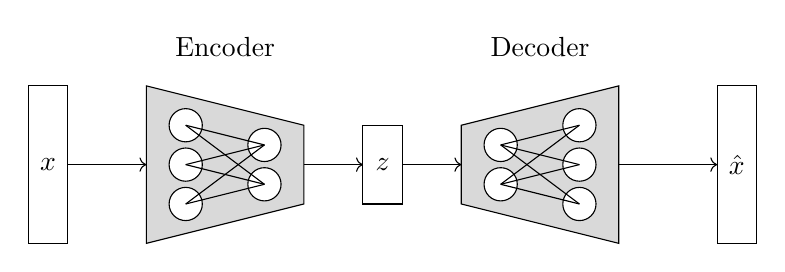
\begin{tikzpicture}
        % Center point of encoder
        \coordinate (E_CENTER) at (1, 1);
        \coordinate (INPUT_TEXT) at (-0.25, 0.5);



        % Draw input vector
        \draw ($(INPUT_TEXT) + (-0.25, -0.5)$) rectangle ($(INPUT_TEXT) + (0.25, 1.5)$) node[pos=.5] {$x$};
        \draw[->] ($(E_CENTER) + (-1, 0)$) -- (E_CENTER);

        








        % Draw the encoder
        \node at ($(E_CENTER) + (1, 1.5)$) {Encoder};
        
        \coordinate (A) at ($(E_CENTER) + (0, -1)$);
        \coordinate (B) at ($(E_CENTER) + (2, -0.5)$);
        \coordinate (C) at ($(E_CENTER) + (2, 0.5)$);
        \coordinate (D) at ($(E_CENTER) + (0, 1)$);
        \draw[fill=gray!30] (A) -- (B) -- (C) -- (D) -- cycle;
        
        % Define the coordinates for the first set of circles (3 neurons)
        \coordinate (n1) at ($(E_CENTER) + (0.5, -0.5)$);
        \coordinate (n2) at ($(E_CENTER) + (0.5, 0)$);
        \coordinate (n3) at ($(E_CENTER) + (0.5, 0.5)$);
        
        % Define the coordinates for the second set of circles (2 neurons)
        \coordinate (m1) at ($(E_CENTER) + (1.5, 0.25)$);
        \coordinate (m2) at ($(E_CENTER) + (1.5, -0.25)$);
        
        % Draw the first set of circles
        \foreach \i in {n1, n2, n3} {
            \filldraw[fill=white] (\i) circle (6pt);
        }
        
        % Draw the second set of circles
        \foreach \i in {m1, m2} {
            \filldraw[fill=white] (\i) circle (6pt);
        }
        
        % Draw arrows from each circle in the first set to each circle in the second set
        \foreach \i in {n1, n2, n3} {
            \foreach \j in {m1, m2} {
                \draw[-] (\i) -- (\j);
            }
        }






        % Draw code vector

        % Arrow in
        \coordinate (Z_TEXT) at ($(E_CENTER) + (3, 0)$);
        \draw[->] ($(E_CENTER) + (2, 0)$) -- ($(Z_TEXT) + (-0.25, 0)$);

        \draw ($(Z_TEXT) + (-0.25, -0.5)$) rectangle ($(Z_TEXT) + (0.25, 0.5)$) node[pos=.5] {$z$};
        
        % Arrow out
        \coordinate (D_CENTER) at ($(E_CENTER) + (4, 0)$);
        \draw[->] ($(Z_TEXT) + (0.25, 0)$) -- (D_CENTER);











        % Draw decoder
        \node at ($(D_CENTER) + (1, 1.5)$) {Decoder};
        
        \coordinate (A2) at ($(D_CENTER) + (0, 0.5)$);
        \coordinate (B2) at ($(D_CENTER) + (2, 1)$);
        \coordinate (C2) at ($(D_CENTER) + (2, -1)$);
        \coordinate (D2) at ($(D_CENTER) + (0, -0.5)$);
        \draw[fill=gray!30] (A2) -- (B2) -- (C2) -- (D2) -- cycle;
        
        % Define the coordinates for the first set of circles (2 neurons)
        \coordinate (n2_1) at ($(D_CENTER) + (0.5, 0.25)$);
        \coordinate (n2_2) at ($(D_CENTER) + (0.5, -0.25)$);
        
        % Define the coordinates for the second set of circles (3 neurons)
        % \coordinate (m2_1) at (1.5, 0.5);
        % \coordinate (m2_2) at (1.5, 1);
        % \coordinate (m2_3) at (1.5, 1.5);
        \coordinate (m2_1) at ($(n2_1) + (1, 0.25)$);
        \coordinate (m2_2) at ($(n2_1) + (1, -0.25)$);
        \coordinate (m2_3) at ($(n2_1) + (1, -0.75)$);
        
        % Draw the first set of circles
        \foreach \i in {n2_1, n2_2} {
            \filldraw[fill=white] (\i) circle (6pt);
        }
        
        % Draw the second set of circles
        \foreach \i in {m2_1, m2_2, m2_3} {
            \filldraw[fill=white] (\i) circle (6pt);
        }
        
        % Draw arrows from each circle in the first set to each circle in the second set
        \foreach \i in {n2_1, n2_2} {
            \foreach \j in {m2_1, m2_2, m2_3} {
                \draw[-] (\i) -- (\j);
            }
        }


        \coordinate (D_END) at ($(D_CENTER) + (2, 0)$);




        % Draw output vector
        \coordinate (X_OUT_TEXT) at ($(m2_2) + (2, 0)$);
        \draw[->] (D_END) -- ($(X_OUT_TEXT) + (-0.25, 0)$);
        
        \draw ($(X_OUT_TEXT) + (-0.25, -1)$) rectangle ($(X_OUT_TEXT) + (0.25, 1)$) node[pos=.5] {$\hat{x}$};
        
        % \node at (X_OUT_TEXT) {$\hat{x}$};
        
    \end{tikzpicture}
    \caption{Autoencoder architecture.}
\end{figure}


More formally, the encoder network takes an input data point $x$ and maps it to a latent space representation $z$, which is compressed representation of $x$. The input is a vector, therefor an image must be flattened from 2D to 1D vector. This flattening will become an issue later in image generation, as this action removes important spatial information and hidden structures in the image. Because of this, modifications were made to the VAE model which allows the capture of spatial information by using a CNN (Convolutional Neural Network) \cite{cnn} layers \cite{vae_cnn_example}, max pooling layers, and more. After compression, the latent vector $z$ is then passed onto the decoder for reconstruction. 

The reconstruction is learned by a reconstruction loss function, usually mean squared error (MSE) loss function:

\begin{equation}
    \text{MSE} = \frac{1}{N} \sum_{i=1}^{N} (y_i - \hat{y}_i)^2
\label{eq:mse}
\end{equation}

The MSE loss is common in image generation models, because this loss is used to ensure that the generated images closely resemble the original input images by comparing the distance between pixels (input image, output image). This objective motivates the model to reconstruct the image from latent vector to resemble the original image. However, this loss is not used alone usually, but in combination with more complex loss functions, as we will see later in VAE.

The code vectors learned by autoencoders, however, are one-to-one map of the input and code vector (deterministic mapping from input to code vectors). The model doesn't capture any semantic relationships between the data (e.g the code vectors of images of cats are scattered throughout the entire latent space, whereas in VAE, they are clustered together). The latent space in autoencoders is irregular and discontinuous, meaning a small change in the latent vector can lead to large unpredictable changes in the output. This makes interpolation in the latent space difficult. Variational autonecoder solve this problem. VAE regularizes the latent space by enforcing a prior distribution. This regularization leads to a smooth and continuous latent space (see figure \ref{fig:ae_vs_vae}), which allows the model to interpolate between the latent space smoothly, thus creating similar new images with different variations. VAEs also provide an explicit model of the data distribution by maximizing a variational lower bound on the likelihood of the data. In other words, VAE is probabilistic model instead of discrete mapper (like the autoencoder model).

\begin{figure}[h]
    \centering
    \includegraphics[scale=0.5]{images/autoencoder-vs-variational-autoencoder-point-vs-distribution-768x409.png}
    \caption{Illustration of mapping an input image to code vector (left) and mapping an input image to a distribution (right) \cite{ae_vs_vae}.}
    \label{fig:ae_vs_vae}
\end{figure}

At the heart of VAE lies the concept of latent variables (Appendix \ref{appendix:latent_variables}). Latent variables are hidden, unobserved variables that the model infers from the observed data (dataset). Latent variable models, such as VAE, take indirect approach to describing a probability distribution $p(x)$ over multi-dimensional variable $x$. Instead of directly writing the expression for $p(x)$, they model a joint distribution $p(x|z)$ of the data $x$ and an unobserved hidden latent variable $z$.

The variational aspect of VAE refers to the use of variational inference (VI) (Appendix \ref{appendix:variational_inference}). VI is used to used to approximate complex posterior distributions: 

\begin{equation}
p(z|x) = \frac{p(x|z) \cdot p(z)}{\int p(x|z) \cdot p(z) dz}
\label{eq:posterior}
\end{equation}

by transforming the problem into optimization problem. The denominator in eq. \ref{eq:posterior} is intractable because it involves integrating over all possible values of $z$, and $z$ is often relatively high-dimensional and its infeasible to evaluate exactly. Which is why VI is used, which approximates the true posterior distribution $p(z|x)$ with simpler, tractable distribution $q_\phi (z|x)$, parameterized by $\phi$.

The original VAE model uses fully connected layers at the encoder and decoder networks. However, in the image synthesis field, CNN layers (appendix \ref{appendix:cnn}) are used instead which are computationally less expensive and better capture the spatial information.

To generate an image, we first sample a latent variable $z$ from prior distribution $p(z)$, which is typically standard normal distribution $\mathcal{N}(0, 1)$. Then $z$ is passed to the decoder an an image $x$ is generated from the conditional distribution $p_\theta (x|z)$. 

\subsection{The Reparameterization Trick}
To enable backpropagation through the sampling process, VAEs use the reparameterization trick. This trick involves expressing the sampled latent variables $z$ as a deterministic function of the encoder's output and some random noise. Without this technique, backpropagation would not be possible through the sampling operation. The reason is that sampling is a non-differentiable operation, because sampling from a distribution involves randomness that does not have a gradient, and the gradients cannot be computed with respect to the parameters of the encoder. To make the sampling operation differentiable and thus allow gradients to flow through the network, the reparameterization trick is used. 

Specifically, if $\mu$ and $\sigma$ are the mean and standard deviation vectors outputted by the encoder, we can write:

\begin{equation}
    z = \mu + \sigma \cdot \epsilon
\end{equation}

where $\epsilon \sim \mathcal{N}(0, 1)$ is a standard normal random variable. This $\epsilon$ will not change throughout the training reigime. It is sampled once and fixed in place. This trick allows us instead of having full stochastic node that blocks flow of gradients, to having two parts: one where we can do backpropagation, and another part which is still stochastic but which we don't want to train because its fixed.


\begin{figure}[h]
    \centering
    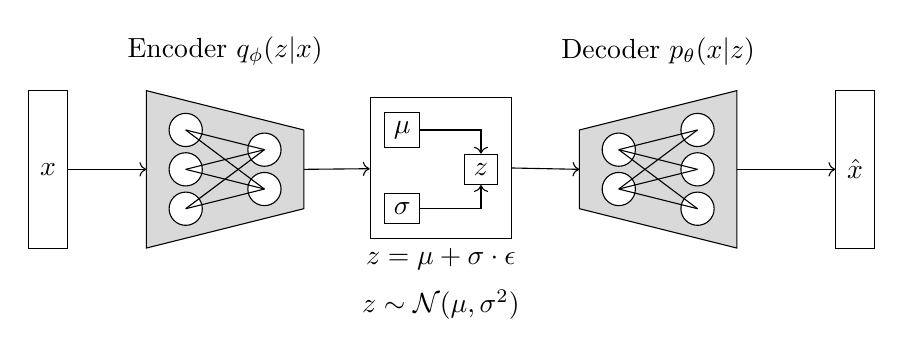
\begin{tikzpicture}
        % Center point of encoder
        \coordinate (E_CENTER) at (1, 1);
        \coordinate (INPUT_TEXT) at (-0.25, 0.5);



        % Draw input vector
        \draw ($(INPUT_TEXT) + (-0.25, -0.5)$) rectangle ($(INPUT_TEXT) + (0.25, 1.5)$) node[pos=.5] {$x$};
        \draw[->] ($(E_CENTER) + (-1, 0)$) -- (E_CENTER);

        








        % Draw the encoder
        \node at ($(E_CENTER) + (1, 1.5)$) {Encoder $q_\phi(z|x)$};
        
        \coordinate (A) at ($(E_CENTER) + (0, -1)$);
        \coordinate (B) at ($(E_CENTER) + (2, -0.5)$);
        \coordinate (C) at ($(E_CENTER) + (2, 0.5)$);
        \coordinate (D) at ($(E_CENTER) + (0, 1)$);
        \draw[fill=gray!30] (A) -- (B) -- (C) -- (D) -- cycle;
        
        % Define the coordinates for the first set of circles (3 neurons)
        \coordinate (n1) at ($(E_CENTER) + (0.5, -0.5)$);
        \coordinate (n2) at ($(E_CENTER) + (0.5, 0)$);
        \coordinate (n3) at ($(E_CENTER) + (0.5, 0.5)$);
        
        % Define the coordinates for the second set of circles (2 neurons)
        \coordinate (m1) at ($(E_CENTER) + (1.5, 0.25)$);
        \coordinate (m2) at ($(E_CENTER) + (1.5, -0.25)$);
        
        % Draw the first set of circles
        \foreach \i in {n1, n2, n3} {
            \filldraw[fill=white] (\i) circle (6pt);
        }
        
        % Draw the second set of circles
        \foreach \i in {m1, m2} {
            \filldraw[fill=white] (\i) circle (6pt);
        }
        
        % Draw arrows from each circle in the first set to each circle in the second set
        \foreach \i in {n1, n2, n3} {
            \foreach \j in {m1, m2} {
                \draw[-] (\i) -- (\j);
            }
        }






        % Draw middle
        \coordinate (Z_TEXT) at ($(E_CENTER) + (3, 0)$);

        \coordinate (MIDDLE_BEGIN) at ($(Z_TEXT) + (-0.5, 0)$);
        \coordinate (MU_BEGIN) at ($(MIDDLE_BEGIN) + (0.25, 0.5)$);
        \coordinate (SIGMA_BEGIN) at ($(MIDDLE_BEGIN) + (0.25, -0.5)$);
        \coordinate (Z_BEGIN) at ($(Z_TEXT) + (0.75, 0)$);

        \coordinate (ARROW_OUT_BEGIN) at ($(Z_TEXT) + (1.75, 0)$);
        \coordinate (ARROW_OUT_END) at ($(ARROW_OUT_BEGIN) + (0.5, 0)$);

        % Middle nodes
        \node[draw,rectangle] (SIGMA) at ($(SIGMA_BEGIN) + (0.5, 0)$) {$\sigma$};
        \node[draw,rectangle] (MU) at ($(MU_BEGIN) + (0.5, 0)$) {$\mu$};
        \node[draw,rectangle] (Z) at ($(Z_BEGIN) + (0.5, 0)$) {$z$};

        % Rectangle around all nodes
        \node[draw, rectangle, inner sep=5pt, fit=(SIGMA) (MU) (Z)] (middle_rect) {};

        % Equations below the rectangle
        \node[below=0cm of middle_rect] (eq1) {$z = \mu + \sigma \cdot \epsilon$};
        \node[below=0cm of eq1] (eq2) {$z \sim \mathcal{N}(\mu, \sigma^2)$};

        % Arrow from trapazoid to rectangle
        \draw[->] ($(E_CENTER) + (2, 0)$) -- (middle_rect);

        % Inner arrows
        \draw[->, to path={-| (\tikztotarget)}] (SIGMA) edge (Z) (MU) edge (Z);











        % Draw decoder
        \coordinate (D_CENTER) at ($(Z_TEXT) + (2.5, 0)$);
        \node at ($(D_CENTER) + (1, 1.5)$) {Decoder $p_\theta(x|z)$};

        % Arrow from the rectangle to the trapezoid
        \draw[->] (middle_rect.east) -- (D_CENTER);

        % Draw trapazoid
        \coordinate (A2) at ($(D_CENTER) + (0, 0.5)$);
        \coordinate (B2) at ($(D_CENTER) + (2, 1)$);
        \coordinate (C2) at ($(D_CENTER) + (2, -1)$);
        \coordinate (D2) at ($(D_CENTER) + (0, -0.5)$);
        \draw[fill=gray!30] (A2) -- (B2) -- (C2) -- (D2) -- cycle;
        
        % Define the coordinates for the first set of circles (2 neurons)
        \coordinate (n2_1) at ($(D_CENTER) + (0.5, 0.25)$);
        \coordinate (n2_2) at ($(D_CENTER) + (0.5, -0.25)$);
        
        % Define the coordinates for the second set of circles (3 neurons)
        \coordinate (m2_1) at ($(n2_1) + (1, 0.25)$);
        \coordinate (m2_2) at ($(n2_1) + (1, -0.25)$);
        \coordinate (m2_3) at ($(n2_1) + (1, -0.75)$);
        
        % Draw the first set of circles
        \foreach \i in {n2_1, n2_2} {
            \filldraw[fill=white] (\i) circle (6pt);
        }
        
        % Draw the second set of circles
        \foreach \i in {m2_1, m2_2, m2_3} {
            \filldraw[fill=white] (\i) circle (6pt);
        }
        
        % Draw arrows from each circle in the first set to each circle in the second set
        \foreach \i in {n2_1, n2_2} {
            \foreach \j in {m2_1, m2_2, m2_3} {
                \draw[-] (\i) -- (\j);
            }
        }


        \coordinate (D_END) at ($(D_CENTER) + (2, 0)$);

        % Draw output vector
        \coordinate (X_OUT_TEXT) at ($(m2_2) + (2, 0)$);
        \draw[->] (D_END) -- ($(X_OUT_TEXT) + (-0.25, 0)$);
        
        \draw ($(X_OUT_TEXT) + (-0.25, -1)$) rectangle ($(X_OUT_TEXT) + (0.25, 1)$) node[pos=.5] {$\hat{x}$};
        
        % \node at (X_OUT_TEXT) {$\hat{x}$};
        
    \end{tikzpicture}
    \caption{Variational Autoencoder architecture.}
    \label{figure:vae}
\end{figure}


The VAE architecture is shown in figure \ref{figure:vae}.

\subsection{Training}

The VAE optimizes the Evidence Lower Bound (ELBO) (see appendix \ref{appendix:elbo}) to ensure that the approximate posterior $q_\phi (z|x)$ is close to the true posterior $p(z|x)$ (we want to maximize it):

\begin{equation}
    \mathcal{L}(\theta, \phi; x, z) = \text{ELBO} = \mathbb{E}_{q_\phi(z|x)} \left[ \log p_\theta(x|z) \right] - D_\text{KL}(q_\phi(z|x) \| p(z))
\end{equation}

where the first term is the reconstruction loss and the second term is the KL divergence (see appendix \ref{appendix:kl_divergence}) (which measure how much the approximate posterior $q_\phi (z|x)$ diverges from the prior $p(z)$). 
\section{VQ-VAE}
\label{sec:vqvae}

Vector Quantized Variational Autoencoder (VQ-VAE) \cite{vqvae} is a generative models based on VAE \ref{sec:vae} model with the addition of vector quantization (VQ) (section \ref{subsec:vqvae_vq}) technique. 

\subsection{Vector Quantization}
\label{subsec:vqvae_vq}

Vector quantization (VQ) is a technique used to discretize continuous data. In the context of VQ-VAE, the continuous latent space $z$ is mapped into discrete codes vectors. In a continuous latent space, the amount of possibilities for a value in the hidden space is infinite, which makes it difficult for the model to learn the hidden space efficiently. With a discrete hidden space, learning becomes more efficient because there is a fixed number of possible values (although in reality it is very large, for example the amount of objects that can be described using language is finite but very large). Furthermore, in reality, images are divided into classes of objects such as cats, people, dogs, etc., and each class has a finite number of possibilities, which is better suited to a discrete latent vectors.

\begin{figure}[h]
    \centering
    \includegraphics[scale=0.5]{images/vq_visualization.png}
    \caption{Illustration of vector quantization discrete clustering of the 2D latent space \cite{vq_visualization_website}. The grey dots are embeddings of the continous latent space, and the red dots are the code vectors from the codebook. In this case, the codebook size is 16.}
    \label{figure:vq_visualization}
\end{figure}

This technique involves the use of a codebook, which is a discrete collection of vectors of the same size as the hidden dimension. In the VQ-VAE model, after the input passes through the encoder (which results in embeddings - which are the hidden representation of the input), the embeddings are replaced by the closest vector from the codebook (by minimizing distance between vectors). This operation allows the model to learn clusters of similar embeddings, which can be used to generate new samples. The codebook is learned during training, and the embeddings are quantized to the nearest code vector in the codebook. The codebook is learned by minimizing the loss function:

\begin{equation}
    \mathcal{L}_{\text{VQ}} = || \text{sg}[z_e] - z_q ||_2^2 + \beta || \text{sg}[z_q] - z_e ||_2^2
\label{eq:vq_loss}
\end{equation}

where $z_e$ is the encoder output, $z_q$ is the quantized output, $\text{sg}[\cdot]$ is the stop gradient operation (which prevents gradients from flowing through the quantization operation), and $\beta$ is a hyperparameter that controls the weighting of the two terms in the loss function. The first term in the loss function is the quantization loss, which measures the distance between the encoder output and the quantized output. The second term is the commitment loss, which measures the distance between the quantized output and the encoder output. The commitment loss encourages the model to use the codebook, and prevents the model from ignoring the quantization operation.

\subsection*{Architecture}

ABC

\subsection*{Training}

ABC
\section{Generative Adversarial Networks (GANs)}

Generative Adversarial Networks (GANs) \cite{gan} are a class of deep learning models that are used to generate new data samples from a given distribution. More specifically, they are very good at synthesizing high-quality images. The model can be used by itself, or as we will see later, it can also be the basis of other image and video generation models, such as VQ-GAN \ref{sec:vqgan}.

\begin{figure}
    \centering
    \resizebox{\textwidth}{!}{
        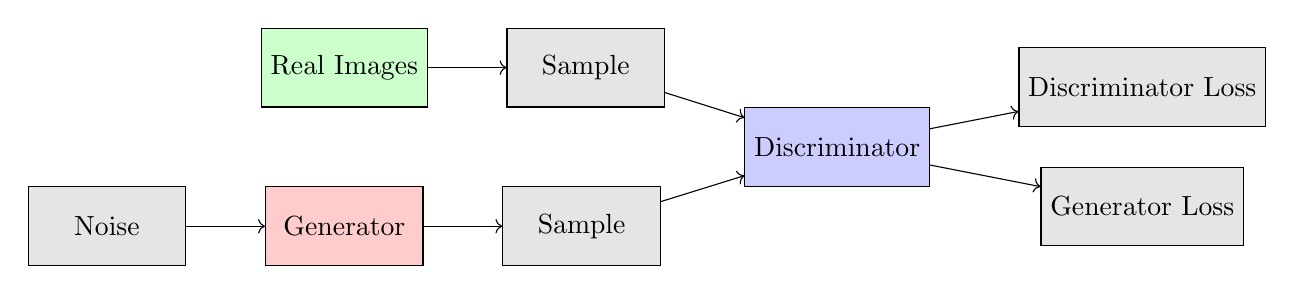
\begin{tikzpicture}
            % Real images, Generator nodes
            \node[rectangle, draw, fill=green!20, minimum width=2cm, minimum height=1cm] (real_images) {Real Images};
            \node[rectangle, draw, fill=red!20, minimum width=2cm, minimum height=1cm, below=of real_images] (generator) {Generator};

            % Noise node
            \node[rectangle, draw, fill=gray!20, minimum width=2cm, minimum height=1cm, left=of generator] (noise) {Noise};

            % Arrow from noise to generator
            \draw[->] (noise) -- (generator);

            % Sample nodes
            \node[rectangle, draw, fill=gray!20, minimum width=2cm, minimum height=1cm, right=of generator] (sample_gen) {Sample};
            \node[rectangle, draw, fill=gray!20, minimum width=2cm, minimum height=1cm, right=of real_images] (sample_real_images) {Sample};

            % Fit sample nodes in a box
            \node[fit=(sample_gen)(sample_real_images), inner sep=0] (sample_fitbox) {};


            % Arrows to sample nodes
            \draw[->] (real_images) -- (sample_real_images);
            \draw[->] (generator) -- (sample_gen);

            % Discriminator node
            \node[rectangle, draw, fill=blue!20, minimum width=2cm, minimum height=1cm, right=of sample_fitbox] (discriminator) {Discriminator};

            % Arrows to discriminator
            \draw[->] (sample_real_images) -- (discriminator);
            \draw[->] (sample_gen) -- (discriminator);

            % Discriminator loss, Generator loss
            % Matrix for the nodes to the right
            \matrix[
                right=of discriminator, 
                column sep=0.5cm, 
                row sep=0.5cm, 
                nodes={rectangle, draw, minimum width=4cm, minimum height=2cm, anchor=center}
            ] (matrix) {
                \node[rectangle, draw, fill=gray!20, minimum width=2cm, minimum height=1cm] (discriminator_loss) {Discriminator Loss}; \\
                \node[rectangle, draw, fill=gray!20, minimum width=2cm, minimum height=1cm] (generator_loss) {Generator Loss}; \\
            };

            % Add arrows
            \draw[->] (discriminator) -- (discriminator_loss);
            \draw[->] (discriminator) -- (generator_loss);
        \end{tikzpicture}
    }
    \caption{High-level overview of GAN architecture \cite{gan}. Noise is sampled from a noise distribution and fed to the generator. The generator outputs an image, and the discriminator needs to decide if the image was generated by the generator or if its an image from the dataset. This decision then affects the value of the loss function, and the weights are updated accordingly by backpropogation.}
    \label{fig:gan_architecture_highlevel}
\end{figure}

% TODO: \ref{fig:gan_architecture} is referencing to the GAN section, and not the figure! WTF
The model consists of two neural networks: a generator $G$ and a discriminator $D$ (as shown in figure \ref{fig:gan_architecture}). The generator is responsible for generating new samples $x$ (images), while the discriminator is responsible for distinguishing between real samples (from the dataset, $D(x) = 1$) and generated samples (fake, from the generator, $D(x) = 0$). The two networks are trained simultaneously in a minimax game (see training section \ref{subsec:gan_training}), where the generator tries to generate samples that are indistinguishable from real samples, and the discriminator tries to distinguish between real and generated samples. The training process continues until the generator is able to generate realistic and high-quality images. 

The noise vector is sampled from a simple distribution like Gaussian. The basic idea of using noise as input is that the model learns to establish relationships between each dimension in the vector and the output image, similar to latent vectors or code vectors. For instance, the model might learn that the first dimension of the noise vector corresponds to the shape of the middle of the image (like the shape of the head of a person), while the second dimension might corresponds to the color of the shape, and so on.




\subsection{Training}
\label{subsec:gan_training}

The loss function of the GAN model is defined as the following min-max game:

\begin{equation}
    \label{eq:gan_loss}
    \min_G \max_D V(D,G) = \mathbb{E}_{x \sim p_{\text{data}}(x)}[\log D(x)] + \mathbb{E}_{z \sim p_z(z)}[\log(1 - D(G(z)))]
\end{equation}

We have two prior distributions: $x \sim p_{\text{data}}$ and $z \sim p_z(z)$, where the noise vector $z$ is sampled from a noise distribution, and $p_{\text{data}}$ represents the true underlying distribution of the dataset, and $x$ is sampled from this distribution.

With respect to the discriminator gradients, the loss function tries to maximize the probability that:

\begin{enumerate}
    \item the discriminator correctly classifies real samples as real (the first term)
    \item the discriminator correctly classifies generated samples as fake (the second term)
\end{enumerate}


With respect to the generator gradients \footnote{When we do backpropogation with respect to the generatoe gradients, the first term is constant.}, the loss function tries to minimize the probability that:

\begin{enumerate}
    \item the generator tries to fool the discriminator in thinking that the generated samples are real (the second term)
\end{enumerate}


The researchers mentioned that at the beginning of the training, the discriminator rejects samples with high confidense. To address this, they suggested instead of \textbf{minimizing} the second term, to \textbf{maximize} a new second term in the loss function: $\log D(G(z))$.


\begin{figure}
    \centering
    \includegraphics[width=0.75\textwidth]{images/gan_training.png}
    \caption{The training algorithm for GAN using minibatch stochastic gradient decent \cite{gan}.}
    \label{fig:gan_training}
\end{figure}

In order to balance of the training for both $G$ and $D$ the authors suggested using iterative approach using minibatch stochastic gradient decent (see figure \ref{fig:gan_training}). Instead of fully optimizing $D$ in each iteration, the algorithm alternates between a few steps ($k$ steps) of optimizing the discriminator and one step of optimizing the generator. By updating $D$ more often the researchers hope to update the generator more slowly and stabilize the training process.



\subsection{Mode Collapse}

One of the main challenges of training GANs is mode collapse. Mode collapse occurs when the generator learns to generate only a few samples, instead of learning to generate a diverse set of samples. This can happen when the generator learns to generate samples that fool the discriminator, but failed to capture the full diversity of the training data distribution (see figure \ref{fig:gan_mode_collapse}). This can happen when the discriminator is too strong, and the generator is not able to generate diverse samples. In other words, the generator tries to fool the discriminator so much that it only focuses on this goal, while ignoring to diversify the samples.

\begin{figure}
    \centering
    \includegraphics[width=\textwidth]{images/gan_mode_collapse.png}
    \caption{Mode collapse in GANs (top row) \cite{gan_mode_collapse_image_source}. Bottom row shows GAN samples without mode-collapse. Blue dots are the prior $x \sim p_{\text{data}}(x)$ and the orange dots are the generated samples $p_g$.}
    \label{fig:gan_mode_collapse}
\end{figure}

\section{VQ-GAN}
\label{vqgan}

\begin{figure}
    \centering
    \includegraphics[width=0.3\textwidth]{images/vqgan_samples.png}
    \caption{Samples generated by VQ-GAN with different resolutions, conditioned on semantic layouts from S-FLCKR dataset \cite{vqgan}.}
\end{figure}


VQ-GAN \cite{vqgan} is a deep learning model for high-quality image generation, combining Vector Quantized Variational Autoencoder (VQ-VAE) \cite{vqvae}, transformers \cite{transformer} (appendix \ref{appendix:transformers}), and Generative Adversarial Network (GAN) \cite{gan} architectures. Its key innovation is representing images as perceptually rich constituents from a codebook rather than raw pixels.

VQ-GAN takes the best of both worlds: the ability to generate high-quality images from GANs and the ability to condition the generation process from VQ-VAE using transformers.

Transformers can learn \textbf{long-range dependencies}, whereas CNNs \cite{cnn} are better fit at learning \textbf{local features} and structures of images.

\begin{figure}
    \centering
    \includegraphics[width=0.6\textwidth]{images/vqgan_architecture.png}
    \caption{VQ-GAN architecture \cite{vqgan}. The bottom rectangular part is the VQ-VAE module with the addition of a discriminator $D$ (right), and the top part is the autoregressive transformer network that predicts the next code vector $s_i$ based on previous outputs $s_{<i}$ \cite{vqgan}.}
    \label{fig:vqgan_architecture}
\end{figure}

In the source code of VQ-GAN the researchers used the \textbf{VGG16} \cite{vgg16} architecture as the backbone of the encoder and decoder networks, but they mentioned that other architectures can be used as well, depending on the generative task. In addition, the authors used the \textbf{minGPT} \cite{mingpt} architecture as the transformer module (more commonly known as \textbf{GPT-2}, which is based on the OpenAI's model GPT-1).

The non-differential operation of quantization is a problem we saw previously in VQ-VAE; to solve this problem the authors said that they used the \textbf{straight-through estimator} (STE) \cite{ste} to backpropagate the gradients through the quantization process, similarly to VQ-VAE.






\subsection{Architecture}

The architecture of VQ-GAN is shown in figure \ref{fig:vqgan_architecture}. The training involves feeding images $x \in X$ of size $x \in \mathbb{R}^{H \times W \times 3}$ \footnote[2]{The training dataset was of size $256 \times 256 \times 3$.} to the encoder $E$ to get the latent representation $\hat{z}$ of size $\hat{z} \in \mathbb{R}^{h \times w \times n_z}$, where $n_z$ is the dimension of each codebook vector. These representations are then quantized by the VQ module to get the discrete latent representation $z_q \in \mathbb{R}^{h \times w \times n_z}$. This operation converts latent vectors to indices of code vectors by nearest neighbor code vector (index in the codebook points to a code vector). Using $z_q$ vectors, the CNN decoder $G$ then reconstructs the image $\hat{x}$. A discriminator $D$ is used to distinguish between real and fake (generated) pixel patches of size 16x16. This module encourages the model to generate finer details and local patterns in the image, leading to better overall quality.

The autoregressive transformer is used to predict the embeddings $z_q$ and provide the decoder $G$ the necessary information to generate a new image, compared to PixelCNN model \cite{pixelcnn} which uses transformer for pixel-by-pixel prediction.




\subsection{Training}

The model is trained in two stages: in the first phase, the VQ module is trained to learn a discrete latent representation of the input data (learn the codebook), and the second phase trains the transformer module to predict the code vectors sequence that will be used to generate the output image.

The loss function of training the model to learn the codebook is given by: (similar to the VQ-VAE loss function in equation \ref{eq:vqvae_loss}):

\begin{equation}
    \mathcal{L}_{\text{VQ}} (E, G, \mathcal{Z}) = \Vert x - \hat{x} \Vert ^2 + \Vert \text{sg}[E(x)] - z_q \Vert ^2_2 +  \beta \Vert \text{sg}[z_q] - E(x) \Vert ^2_2
\end{equation}

where the first term is the MSE reconstruction loss (similar to equation \ref{eq:mse}), the second term is the quantization error, and the third term is the commitment loss. The reconstruction loss is intended to train the decoder $G$ to output (reconstruct latents $z_q$ to an image) images of similar distribution to the dataset. The quantization loss encourages the model to move the codebook vectors towards the encoder outputs, so to match the encoder's output distribution (gradients are calculated for $z_q$ and not $\text{sg}[E(x)]$ because of the stop gradient operation). The commitment loss encourages the encoder to "commit" to outputting embeddings that are close to the codebook vectors.

However, instead of the MSE loss, the authors used a perceptual loss \cite{perceptual_loss} \footnote[4]{Perceptual loss measures the difference between the high-level features of two images (a generated image and an image from the dataset). Typically the high-level features are extracted by pretrained CNNs.} and \textbf{introduced an adversarial training procedure with a patch-based discriminator $D$} that tries to distinguish between real and fake pixel patches of size 16x16 of an image. The loss function of the discriminator is given by:

\begin{equation}
    \mathcal{L}_{\text{GAN}}(\{E,G,Z\}, D) = [\log D(x) + \log (1-D(\hat{x}))]
\end{equation}

If $D$ outputs 1, then the image is from the dataset (real), and if it outputs 0, then the image is fake (generated by the decoder $G$). Just like in GAN, the discriminator objective is to maximize the probability of assigning the correct label to the input image and in the loss function the first term encourages the discriminator to output 1 because $\log D(x)$ approaches 0 when $D(x)$ approaches 1, and the second term encourages the discriminator to output 0 for fake images because $\log (1-D(\hat{x}))$ approaches 0 when $D(\hat{x})$ approaches 0.

Combining both the VQ loss and the adversarial loss, the total loss function is given by:

\begin{equation}
    \mathcal{Q^*} = \arg \min_{E, G, Z} \max_D \mathbb{E}_{x \sim p(x)} [\mathcal{L}_{\text{VQ}} + \lambda \mathcal{L}_{\text{GAN}}]
\end{equation}

The $\lambda$ hyperparameter is used to balance the contribution of adversarial loss relative to the VQ loss.

\begin{figure}
    \centering
    \includegraphics[width=0.5\textwidth]{images/vqgan_samples2.png}
    \caption[Caption for LOF]{Samples generated by VQ-GAN by different tasks and different resolutions. From top to bottom: depth-to-image on RIN dataset, stochastic super resolution\footnotemark on RIN dataset, 3rd and 4th row are semantic synthesis (semantic masks) on S-FLCKR dataset, and bottom row are edge synthesis on IN dataset.}
\end{figure}


\footnotetext{Super resolution is a task that generates high-resolution image from a single low-resolution image while maintaining the spatial information of the image.}

The second phase of the training involves maximizing the transformer objective. The transformer learns to predict the distribution of possible next indices, which allows us to directly maximize the log-likelihood (appendix \ref{appendix:likelihood_function}) of the data representation:

\begin{equation}
    \mathcal{L}_{\text{transformer}} = \mathbb{E}_{x \sim p(x)} [- \log p(x)]
\end{equation}

To summarize, the VQ-GAN model has 3 loss functions: the VQ loss (which trains the model to learn the codebook vectors), the adversarial loss (which trains the model to generate realistic images), and the transformer loss (which trains the model to predict the next code vector autoregressively).







\subsection{Conditional generation}

\begin{figure}
    \centering
    \caption{The conditioned input sequence given to the transformer, based on the spatial condition information $c$. The middle rectangle represents a 'begin sequence' token.}
    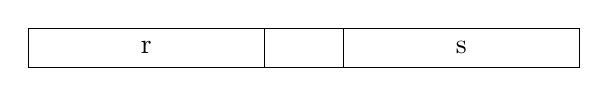
\begin{tikzpicture}
        \def \rectheight{0.5}

        % Draw the first rectangle
        \draw (0,0) rectangle (3,\rectheight);
        \node at (1.5,\rectheight / 2) {r};
        
        % Draw the middle rectangle
        \draw (3,0) rectangle (4,\rectheight);
        
        % Draw the third rectangle
        \draw (4,0) rectangle (7,\rectheight);
        \node at (5.5,\rectheight / 2) {s};
    \end{tikzpicture}
    \label{fig:vqgan_conditional_generation}
\end{figure}

% TODO: Finish
After the two-phase training is finished, the transformer is used to predict a sequence $s$ which is sequence of indices to code vectors. Each token $s_i$ corresponds to an index in the codebook. So a code vector is autoregressively predicted based on the previous tokens $s_{<i}$, which provides the necessary embeddings $z_q$ for image synthesis ($p(s) = \prod_{i} p(s_i | s_{<i})$). If the image generation process involves a condition basis $c$, such as text, images, depth map, semantic layout or pose, then another VQ-GAN model is trained on these kind of tasks, which obtain a new codebook $Z_c$ which are the representation $r$ of $c$. Then, this representation is prepended to $s$ which restricts the computation of the negative log-likelihood to entries $p(s_i | s_{<i}, r)$. This new sequence is then given to the transformer in the first model to generate the image based on the condition $c$ (figure \ref{fig:vqgan_conditional_generation}).








\subsection{Sliding window technique for generating high-resolution images}

\begin{figure}[h]
    \centering
    \includegraphics[width=0.75\textwidth]{images/vqgan_sliding_attention.png}
    \caption{Sliding window attention technique for generating high-resolution images. The output image is divided into patches of size 16x16=256 and by using attention mechanism, the transformer module is able to autoregressively generate the next code vector $s_i$ based on the previous outputs $s_{<i}$ (the context).}
    \label{fig:vqgan_sliding_window}
\end{figure}

Due to the attention mechanism in transformers (quadratic computation for number of tokens, because each token requires attention to all other tokens), the model is limited in the size of the transformer sequence (in the paper they used 256 tokens). Although the encoder can reduce the dimensionality of images, the researchers noticed significant degradation in generation quality. To solve this problem, they work patch-wise and crop input images to match the maximum token count in the transformer module.

To sample images, they also work patch-wise and the transformer autoregressively predicts the next token based on the window context (figure \ref{fig:vqgan_sliding_window}).



% Diffusion models
\section{Denoise Diffusion Probabilistic Models (DDPMs)}


\subsection{Diffusion Models (DMs)}
\label{subsec:diffusion_models}

Diffusion models are probabilistic generative models that map latent variables to observed data. Unlike GANs, they are easier to train and can produce high-quality images by progressively adding and removing noise. Most importantly, this model serves as a basis to other generative models.

A diffusion model consists of:

\begin{itemize}
    \item An encoder that maps the data $x$ through stochastic intermediate latent variables $z_1, ..., z_T$.
    \item And a decoder reversing the noising process
\end{itemize}








\subsection{DDPMs}
\label{sec:ddpm}

Denoise Diffusion Probabilistic Models (DDPMs) \cite{ddpm} are a class of diffusion models that are trained to denoise images by reconstructing a noised image. 

There are two processes, each process takes multiple ($t$) steps:

\begin{itemize}
    \item \textbf{Forward diffusion process}: Adds noise to the input image\footnote{There are multiple implementations on how to add noise to image. The simplest way is to use random values for each pixel (\texttt{torch.randn\_like()}) by tensor addition, but the most common way is to use Gaussian noise which distributes the noise normally (\texttt{np.random.normal(mean, sigma, ...)}).}. The addition of noise is the addition of random pixel values to the input image. In forward diffusion, we transform the image $x$ (from the dataset, without noise) to a latent variable $z_0 = x$. Then we add noise to get $z_1$, and so on, until $t$ steps we get $z_t$ - which is pure noise image, distributed from the noise distribution (usually Gaussian). The forward diffusion step is denoted as $\mathbf{q(x_t | x_{t-1})}$.
    
    \item \textbf{Reverse diffusion process}: Removes noise from the input noised image. The removal of noise can be thought as adding new features to the image. In reverse diffusion, we transform the image $z_t$ to $z_{t-1}$ by removing noise in a single step. We repeat this process until we get the original image $x = z_0$. The reverse diffusion step is denoted as $\mathbf{p_\theta (x_{t-1} | x_t)}$.
\end{itemize}

Because the addition of noise is a known stochastic process, \textbf{all the learned parameters are in the decoder} (the generator). We don't want to learn the addition of noise, since the task is to denoise the image. DDPMs learn with a fixed inference procedure $q(x_{1:T} | x_0)$.

DDPMs are latent variable models in the form of:

\begin{equation*}
    p_\theta (x_0) = \int p_\theta(x_{0:T}) dx_{1:T} \text{,\ \ where \ \ \ } p_\theta (x_{0:T}) := p_\theta (x_T) \prod_{t=1}^{T} p_\theta (x_{t-1} | x_t)
\end{equation*}

Because this \textbf{integral is intractable}, we use ELBO. The parameters of the model $\theta$ are learned to fit the data distribution $q(x_0)$ by \textbf{maximizing a variational lower bound}:

\begin{equation*}
    \max_{\theta} \mathbb{E}_{q(x_0)} [\log p_\theta (x_0)] \leq \max_\theta \mathbb{E}_{q(x_0, x_1, ..., x_T)} [\log p_\theta (x_{0:T}) - \log q(x_{1:T} | x_0)]
\end{equation*}

where $q(x_{1:T} | x_0)$ is the reverse diffusion process over the latent variables.


\begin{figure}
    \centering
    \includegraphics[width=1\textwidth]{images/diffusion_models/ddpm_denoise.png}
    \caption{Progressive generation (left to right) of unconditional CIFAR10 dataset in DDPM \cite{ddpm}.}
\end{figure}


\begin{figure}
    \centering
    \includegraphics[width=0.7\textwidth]{images/diffusion_models/ddpm_process.png}
    \caption{A graph representing the forward ($q(x_t | x_{t-1})$) and reverse ($p_\theta(x_{t-1} | x_t)$) diffusion process in DDPMs \cite{ddpm}. The next step (either in forward or reverse diffusion) depends conditionally on the previous steps (Markov chains) \cite{ddpm}.}
    \label{fig:ddpm_process}
\end{figure}






\begin{figure}[h]
    \centering
    \begin{minipage}{0.10\textwidth}
        \centering
        \includegraphics[width=\textwidth]{images/diffusion_models/noise_to_image_gif/0.png}
    \end{minipage}
    \begin{minipage}{0.10\textwidth}
        \centering
        \includegraphics[width=\textwidth]{images/diffusion_models/noise_to_image_gif/1.png}
    \end{minipage}
    \begin{minipage}{0.10\textwidth}
        \centering
        \includegraphics[width=\textwidth]{images/diffusion_models/noise_to_image_gif/2.png}
    \end{minipage}
    \begin{minipage}{0.10\textwidth}
        \centering
        \includegraphics[width=\textwidth]{images/diffusion_models/noise_to_image_gif/3.png}
    \end{minipage}
    \begin{minipage}{0.10\textwidth}
        \centering
        \includegraphics[width=\textwidth]{images/diffusion_models/noise_to_image_gif/4.png}
    \end{minipage}
    \begin{minipage}{0.10\textwidth}
        \centering
        \includegraphics[width=\textwidth]{images/diffusion_models/noise_to_image_gif/5.png}
    \end{minipage}
    \begin{minipage}{0.10\textwidth}
        \centering
        \includegraphics[width=\textwidth]{images/diffusion_models/noise_to_image_gif/6.png}
    \end{minipage}
    \begin{minipage}{0.10\textwidth}
        \centering
        \includegraphics[width=\textwidth]{images/diffusion_models/noise_to_image_gif/7.png}
    \end{minipage}
    \caption{Progressive denoising of latents in DDPM. Images taken from the \href{https://scholar.harvard.edu/binxuw/classes/machine-learning-scratch/materials/stable-diffusion-scratch}{harvard university} website.}
\end{figure}






\subsection{Noise Schedulers}

A noise scheduler defines how noise is added to the image at each timestep (for the forward process in DDPMs). Instead of adding noise all at once, a scheduler defines how much noise to add periodically (in steps).

Typically, we control noise schedulers with two parameters: $\alpha_t$ which controls how much noise is added (strength of the noise) at step $t$, and $\beta_t$ which controls the variance  of the noise added at step $t$ (typically referred to as just 'noise schedule' or 'variance').

In the paper \cite{ddpm} the authors used linear scheduler, however OpenAI released a paper \cite{openai_improved_ddpm} that uses cosine scheduler. They have shown that a cosine scheduler performs better than a linear scheduler in terms of image generation quality (see figure \ref{fig:linear_cosine_scheduler}).

\begin{figure}
    \centering
    \includegraphics[width=1\textwidth]{images/diffusion_models/linear_cosine_scheduler.png}
    \caption{\textit{Top}: Linear scheduler \cite{ddpm}; \textit{Bottom}: cosine scheduler \cite{openai_improved_ddpm}. The linear scheduler adds noise too quickly which degrades the model's performance quickly, whereas cosine scheduler adds noise more slowly \cite{openai_improved_ddpm}.}
    \label{fig:linear_cosine_scheduler}
\end{figure}

A variance schedule is simply a function that defines the variance at each given timestep during the forward diffusion process. At each timestep, Gaussian noise $\epsilon$ is added to the previous latent variable:

\[
    x_{t+1} = \sqrt{1 - \beta_t} x_t + \sqrt{\beta_t} \epsilon
\]

Notice that when $\beta$ increases linearly, the term $\sqrt{1-\beta}$ decreases linearly. 

A noise scheduler is a function: $\beta(t):[1, ..., T] \rightarrow \mathbb{R}$ that determines the amount of noise added at each step. Its a sequence of $\alpha_t$.

A \textbf{linear scheduler} \textbf{linear scheduler} is defined as:
\[
    \beta_t = c \cdot t \text{, where c is constant}
\]

and a \textbf{cosine-beta scheduler} can be defined as:

\[
    \bar{\alpha}_t = \frac{f(t)}{f(0)} \text{, where } f(t) = \cos^2 \left( \frac{t/T + s}{1+s} \cdot \frac{\pi}{2} \right)
\]








\subsection{Encoder}

The forward diffusion process maps a data image $x$ through a series of intermediate variables $z_1, ..., z_T$ with the dimension as $x$ according to the following recursion:

\begin{equation}
    \begin{aligned}
    \mathbf{z}_1 &= \sqrt{1 - \beta_1} \cdot \mathbf{x} + \sqrt{\beta_1} \cdot \epsilon_1, \\
    &\;\;\vdots \notag \\
    \mathbf{z}_t &= \sqrt{1 - \beta_t} \cdot \mathbf{z}_{t-1} + \sqrt{\beta_t} \cdot \epsilon_t \quad \forall \, t \in \{2, \ldots, T\}
    \end{aligned}
\end{equation}

At each step $i \in \{1, 2, ..., t, t+1, ..., T\}$ a noise vector $\epsilon_i$ is drawn from a standard normal distribution. This equation adds random noise $\epsilon_i$ to the image $x = z_0$ and $\beta$ is a schedule function ($\beta(t):[1, ..., T] \rightarrow \mathbb{R}$) that determines the amount of noise added at each step ($\beta$ is a variance schedule, which can be linear, cosine, quadratic and more). 

A more formal notation for the \textbf{forward diffusion process} is:

\begin{equation*}
    \begin{aligned}
        q(x_t | x_{t-1}) = \mathcal{N}(x_t; \sqrt{1-\beta_t} \cdot x_{t-1}, \beta_t \mathbf{I}) \\
        q(x_{1:T} | x_0) = \prod_{t=1}^{T} q(x_t | x_{t-1})
    \end{aligned}
\end{equation*}

\begin{itemize}
    \item The noise is sampled from a normal distribution $\epsilon \sim \mathcal{N}(0, 1)$.
    \item The latent variable $x_t$ is sampled from a normal distribution $\mathcal{N}$ where:
    \begin{itemize}
        \item The mean is $\sqrt{1-\beta_t} \cdot x_{t-1}$.
        \item The variance is $\beta_t \mathbf{I}$.
        \item The $\beta$ parameter is the noise scheduler (how much noise we add at each step).
    \end{itemize}
\end{itemize}



\subsubsection*{Skipping intermediate steps in forward diffusion}


An interesting point the authors made is that in forward diffusion it is possible to sample $x_t$ from any arbitrary timestep $t$, given the original image $x_0$ (without calculating all the intermediate steps):

\begin{equation}
    \begin{aligned}
    q(\mathbf{x}_t|\mathbf{x}_0) = \mathcal{N}(\mathbf{x}_t; \sqrt{\bar{\alpha}_t}\mathbf{x}_0, (1 - \bar{\alpha}_t)\mathbf{I}) \\
    \text{where } \alpha_t := 1 - \beta_t \text{ and } \bar{\alpha}_t := \prod_{i=1}^{t} \alpha_i
    \end{aligned}
    \label{eq:forward_diffusion}
\end{equation}

Since $\alpha$ depends on $\beta$ we can see that \textbf{there are no parameters to learn in the forward diffusion process}.

After plugging in $\alpha = 1 - \beta$ in the encoder and the \textbf{reparametrization trick} (from VAE: $\mathcal{N} (\mu, \sigma^2) = \mu + \sigma \cdot \epsilon \text{, where } \epsilon \sim \mathcal{N}(0, 1) $) we get:

\begin{align*}
    q(x_t | x_{t-1}) &= \mathcal{N} \left( x_t; \sqrt{1-\beta_t} x_{t-1}, \beta_t \mathbf{I} \right) \\
    &= \sqrt{1-\beta_t} x_{t-1} + \sqrt{\beta_t} \epsilon_t \\
    &= \sqrt{\alpha_t} x_{t-1} + \sqrt{1 - \alpha_t} \epsilon \\
    &= \sqrt{\alpha_t \alpha_{t-1}} x_{t-2} + \sqrt{1 - \alpha_t \alpha_{t-1}} \epsilon \\
    &= \sqrt{\alpha_t \alpha_{t-1} \alpha_{t-2}} x_{t-3} + \sqrt{1 - \alpha_t \alpha_{t-1} \alpha_{t-2}} \epsilon \\
    &= \sqrt{\alpha_t \alpha_{t-1} \cdots \alpha_1 \alpha_0} x_0 + \sqrt{1 - \alpha_t \alpha_{t-1} \cdots \alpha_1 \alpha_0} \epsilon \\
    &= \boxed{ \sqrt{\bar{\alpha}} x_0 + \sqrt{1 - \bar{\alpha}} \epsilon }
\end{align*}

as a result we get:

\begin{equation}
    q(x_t | x_0) = \mathcal{N} (x_t; \sqrt{\bar{\alpha_t}} x_0, (1-\bar{\alpha_t}) \mathbf{I})
    \label{eq:forward_diffusion_single_step}
\end{equation}

Equation \ref{eq:forward_diffusion_single_step} describes how in a single step we can get a noisier image $x_t$ from the original image $x_0$ without calculating all the intermediate steps. This is a very useful property of latent diffusion models.









\subsection{Decoder}

The decoder removes noise from the intermediate latent variables $z_T, ..., z_1$ and reconstructs the original image $x = z_0$ using the following recursion:

\begin{equation}
    p_\theta(\mathbf{x}_{t-1} | \mathbf{x}_t) = \mathcal{N}(\mathbf{x}_{t-1}; \mu_\theta(\mathbf{x}_t, t), \Sigma_\theta(\mathbf{x}_t, t))
    \label{eq:reverse_diffusion}
\end{equation}

where $\theta$ are the learned parameters of the model. The mean $\mu_\theta$ and variance $\Sigma_\theta$ are unknown and should be learned in the training. 


\subsubsection*{Learning the variance}

In the DDPM paper \cite{ddpm} the authors said:

\begin{quote}
    \textit{"We also see that learning reverse process variances (by incorporating a parameterized diagonal $\Sigma_\theta(x_t)$ into the variational bound) leads to unstable training and poorer sample quality compared to fixed variances."} \cite{ddpm}
\end{quote}

The OpenAI team released a paper titled "Improved denoising diffusion probabilistic models" \cite{openai_improved_ddpm} in which the authors used cosine noise (instead of linear in the original paper \cite{ddpm}) scheduler and also \textbf{learned the variance}, which significantly improved the model's performance.








\subsection{Loss function}

Diffusion models are in the form of $p_\theta (x_0) := \int p_\theta(x_{0:T}) d\mathbf{x}_{1:T}$ which is intractable, thus we use the ELBO loss function to approximate the likelihood of the data.

We seek to train the model to predict the noise $\epsilon_i$ added at each timestep. We could start with a simple loss function (\textbf{negative log likelihood}):

\[ -\log (p_\theta (x_0)) \]

but that's a problem, the probability of $x_0$ depends on all timesteps $x_0, x_1, ..., x_T$. As a solution, loss function of DDPMs is typically the \textbf{variational lower bound} of this objective:

\[
    -\log (p_\theta(x_0)) \leq -\log (p_\theta(x_0)) + D_{KL} (q(x_{1:T} | x_0)) \vert \vert p_\theta(x_{1:T} | x_0)
\]

We can rewrite the KL-divergence as \footnote{Thanks in part for the math explanation to \href{https://www.youtube.com/watch?v=HoKDTa5jHvg}{a youtube video that explained the math in the paper}.}:

\begin{align*}
    D_{KL} (q(x_{1:T} | x_0)) \vert \vert p_\theta(x_{1:T} | x_0) &= \log(\frac{q(x_{1:T} | x_0)}{p_\theta(x_{1:T} | x_0)}) \\
    &= \log(\frac{q(x_{1:T} | x_0)}{ \frac{p_\theta(x_0 | x_{1:T}) p_\theta(x_{1:T})}{p_\theta(x_0)} }) \\
    &= \log(\frac{q(x_{1:T} | x_0)}{ \frac{p_\theta(x_0, x_{1:T})}{p_\theta(x_0)} }) \\
    &= \log(\frac{q(x_{1:T} | x_0)}{ \frac{p_\theta(x_{0:T})}{p_\theta(x_0)} }) \\
    &= \log(\frac{q(x_{1:T} | x_0)}{ p_\theta(x_{0:T}) }) + \log(p_\theta(x_0))
\end{align*}

By reformulating the KL-divergence we arrive at the following loss objective (the terms $-\log(p_\theta(x_0))$ and $\log(p_\theta(x_0))$ cancel each other out):

\begin{align*}
    -\log (p_\theta(x_0)) &\leq -\log (p_\theta(x_0)) + \log (\frac{ q(x_{1:T} | x_0) }{ p_\theta (x_{0:T}) }) + \log(p_\theta(x_0)) \\
    &= \log (\frac{ q(x_{1:T} | x_0) }{ p_\theta (x_{0:T}) }) \\
\end{align*}

we finally get the \textbf{variational lower bound (ELBO)}:

\[
\begin{tikzcd}
    \textcolor{green}{-\log(p_\theta(x_0))} \leq \log(\frac{\textcolor{red}{q(x_{1:T} | x_0)}}{\textcolor{blue}{p_\theta(x_{0:T})}})
    \arrow[d, ""] \\
    \boxed{
        \mathcal{L} = 
        \underbrace{\mathbb{E}[
            \textcolor{green}{-\log p_\theta (x_0)}
        ] }_{\text{NLL}}
        \leq 
        \underbrace{\mathbb{E}_q[-\log (\frac{
            \textcolor{blue}{p_\theta(x_{0:T})}
        }{
            \textcolor{red}{q(x_{1:T}|x_0)}})]}_{\text{ELBO}
        }
    }
\end{tikzcd}
\]

The dominator $\textcolor{red}{q(x_{1:T}|x_0)}$ is the forward diffusion process (adds noise) and the numerator $\textcolor{blue}{p_\theta(x_{0:T})}$ is the reverse process. 

The ratio of these two terms is the ELBO loss function and when this ratio reaches 1, it indicates that the model can undo the forward process. We also don't write $q_\theta$ because the forward process is not learned, only the reverse process is learned.

We can simplify the training objective of DDPMs as simply \textbf{noise predictor} - commonly written as $\epsilon$-prediction:

\begin{equation}
    \boxed{\mathcal{L}_\text{simple} (\theta) = \mathbb{E}_{t,x_0, \epsilon} \left[ \left| \left| \epsilon - \epsilon_\theta (x_t, t) \right| \right|^2 \right]}
    \label{eq:ddpm_loss}
\end{equation}

where $\epsilon_\theta (x_t, t)$ is the noise predicted by the model, given timestep $t$ and noisy input $x_t$.







\subsection{Training}

The training of diffusion models is done by sampling a batch of images from the dataset, and then adding noise to the images in the forward diffusion process. The model is trained to remove the noise and reconstruct the original image in the reverse diffusion process. The loss function is the ELBO loss function. Usually, the model is trained using stochastic gradient descent (SGD), but more advanced optimizers like Adam can be used as well.





\begin{algorithm}
    \caption{The training algorithm of diffusion models \cite{ddpm}.}
    \label{alg:ddpm_training}
    \begin{algorithmic}[1] % Enables line numbering
        \State \textbf{repeat}
        \State \hspace{5pt} $ \mathbf{x}_0 \sim q(\mathbf{x}_0) $
        \State \hspace{5pt} $ t \sim \text{Uniform}(\{1, \dots, T\}) $
        \State \hspace{5pt} $ \epsilon \sim \mathcal{N}(\mathbf{0}, \mathbf{I}) $
        \State \hspace{5pt} Take gradient descent step on
        \[
        \nabla_{\theta} \left\| \epsilon - \epsilon_{\theta} \left( \sqrt{\bar{\alpha}_t} \mathbf{x}_0 + \sqrt{1 - \bar{\alpha}_t} \epsilon, t \right) \right\|^2
        \]
        \State \textbf{until} converged
    \end{algorithmic}
\end{algorithm}





In algorithm \ref{alg:ddpm_training} line 2, we take a sample from the dataset. In line 3, we generate random number between 1 and T uniformly. In line 4, we sample some noise. Line 5: we calculate the gradients of the loss function: we try to optimize the model's parameters $\theta$ by gradient decent. $\epsilon_\theta$ is the predicted noise added at timestep $t$ (a function approximator with 2 parameters that intends to predict $\epsilon$ from $x_t$) where the first parameter is the noisy image at timestep $t$, and the second parameter is the timestep $t$.




\section{Stable Diffusion}
\label{sec:stable_diffusion}


\begin{figure}
    \centering
    \includegraphics[width=0.8\textwidth]{images/diffusion_models/stable_diffusion/stable_diffusion.png}
    \caption{Stable diffusion scales better compared to other models \cite{stable_diffusion} (DALL-E, VQGAN) with less downsampling blocks (4 instead of 16 as needed by VQGAN).}
\end{figure}


Stable diffusion models are based on latent diffusion. In the paper \cite{stable_diffusion} the authors suggested that computing gradients directly on the pixel space is inefficient, since this space is high-dimentional and includes imperceptible details (high-frequency undesired details). Instead, they suggest to first convert the training images to a lower-dimensional latent space and then apply the diffusion processes on this space. The computation is done on the latent space instead of the pixel space. The authors showed that this approach scales better to higher dimension inputs, and showed significant competitive performance on multiple tasks while lowering significantly computational costs.  And finally, the authors introduced general purpose conditioning mechanism based on cross-attention which allows multi-modal training.

% This process is much more efficient, and in the paper \cite{stable_diffusion} the authors showed that the model can be trained on a single GPU with 16GB of memory. The model is trained on a 256x256 resolution CelebA-HQ dataset with 30 diffusion steps.

% An example of this is when giving an image to a person and asking them to describe the image, they will not describe the individual pixel values, but instead describe the high-level features of the image first.

A 2021 paper released by OpenAI \cite{openai_diffusion_beats_gans} shows that diffusion models can outperform GANs in terms of image fidelity by trading off diversity.














\subsection{U-Net backbone}
\label{subsec:stable_diffusion_u_net_backbone}

U-Net (first introduced in 2015) \cite{unet} is a convolutional neural network architecture that is commonly used in diffusion models, particularly in stable diffusion models and its variants. U-Net is used as a backbone for denoising the latent representations. The U-Net architecture is a symmetric encoder-decoder network with skip connections between the encoder and decoder. The skip connections help the network to learn better (by minimizing \textbf{exploding / vanishing gradient problem} \cite{exploding_vanishing_gradients}), the downsampling process of the encoder removes abstract features in the data, and so skip connections allow the model to skip these downsampling blocks and preserve high-level features. In the original DDPM paper \cite{ddpm} the authors didn't explicitly used U-Net, however they used CNN with residual blocks, which is similar in structure and intent to U-Net. 

\begin{figure}
    \centering
    \includegraphics[width=0.8\textwidth]{images/diffusion_models/stable_diffusion/u-net-architecture.png}
    \caption{U-Net architecture \cite{unet}, with convolutional and deconvolutional layers, and skip connections. This architecture is commonly used in stable diffusion models.}
    \label{fig:unet_architecture}
\end{figure}

In figure \ref{fig:unet_architecture} the U-Net is shaped like a 'U' - notice that the layers downsample the input one after the other. Then, after we get to the desired depth, we start upsampling the input until we get output with the same dimensions as the input. The blue arrows are the convolutional layers with kernel size 3x3 and ReLU activation function. The max-pooling are the downsampling layers, and the upsampling layers are the deconvolutional layers.

In addition, the UNet backbone contains \textbf{timestep embeddings}. The scalar timestep (which can be in the range $[0, T]$, where $T$ is the total number of diffusion steps) is first projected into a sinusoidal embedding, similar to the way positional encodings are used in transformers. The timestep embeddings are used to let the model know which step its in the diffusion process currently, this way it knows if its in the beginning of the diffusion or at the late stage, which is essential for removing noise.

\begin{figure}[h]
    \centering
    \includegraphics[width=0.25\textwidth]{images/diffusion_models/stable_diffusion/positional_encodings.png}
    \caption{Sinusoidal positional embeddings used in a transformer model \cite{understanding_deep_learning_book_2024}. It is similar to the timestep embeddings used in stable diffusion U-Net backbone. The X axis is the position of the input sequence (or timestep). The Y axis is the embeddings dimensions. The pattern is sinusodial, lighter regions indicate lower value, darker regions indicate higher values. Its important to note that each column in the X axis is a unique encodings, which helps distinguish the position / timestep of the input sequence.}
\end{figure}

In other words, the U-Net denoises the latent space, and the VAE decoder takes in the denoised latent vectors and generates image based on the latent vectors.

\begin{lstlisting}[language=Python, caption={Timestep embeddings of Stable Diffusion pipeline. We convert the timestep to sinusoidal vector embedding.}, label={lst:timestep_embeddings_stable_diffusion}]
def get_time_embedding(timestep):
    # Shape: (160,)
    freqs = torch.pow(10000, 
        -torch.arange(start=0, end=160, dtype=torch.float32) / 160) 
    # Shape: (1, 160)
    x = torch.tensor([timestep], 
        dtype=torch.float32)[:, None] * freqs[None]
    # Shape: (1, 160 * 2)
    return torch.cat([torch.cos(x), torch.sin(x)], dim=-1)
\end{lstlisting}

The general formula for timestep embeddings is given in equation \ref{eq:timestep_embeddings}. The code snippet in listing \ref{lst:timestep_embeddings_stable_diffusion} is taken from \href{https://github.com/hkproj/pytorch-stable-diffusion/blob/e0cb06de011787cdf13eed7b4287ad8410491149/sd/pipeline.py#L164}{a re-implementation of Stable Diffusion}.

\begin{equation}
    \text{Enc}_i(t) =
    \begin{cases}
        \sin\left(\frac{t}{10000^{\frac{2i}{d}}}\right) & \text{if } i \text{ is even} \\
        \cos\left(\frac{t}{10000^{\frac{2i}{d}}}\right) & \text{if } i \text{ is odd}
    \end{cases}
    \label{eq:timestep_embeddings}
\end{equation}








\subsection{Architecture}

The stable diffusion model, which is a latent diffusion model (LDM), consists of: variational autoencoder which compresses the input images into regularized latent space as an image encoder, a U-Net backbone which denoises the output from forward diffusion backwards to obtain a latent representation (it predicts the noise added in each step), a variational autoencoder decoder which converts the latent representation back to the image space, and an optional classifier-free guidance mechanism which allows the model to be conditioned on text prompts or other images, which is domain-specific encoder. The high level architecture is shown in figure \ref{fig:stable_diffusion_architecture}.

The most popular conditioning mechanism is text prompts. For text, we use text encoder (tokenizer) which converts the text words to vectors / embeddings (tokens). In Stable Diffusion paper, the authors used a \href{https://github.com/CompVis/latent-diffusion/blob/a506df5756472e2ebaf9078affdde2c4f1502cd4/ldm/modules/encoders/modules.py#L138}{frozen CLIPTokenizer}, which is a pre-trained tokenizer trained on specific vocabulary and special tokens (beginning of sentence, end of sentence, padding, mask tokens and more). Although in the source code you will find other text encoders as well, such as BERT \cite{bert}.

\begin{figure}
    \centering
    \includegraphics[width=0.75\textwidth]{images/diffusion_models/stable_diffusion/architecture.png}
    \caption{Stable diffusion architecture \cite{stable_diffusion}. The 'switch' in the diagram is used for different applications of conditional information. In the case of text, they use cross-attention. If the conditional information is another image, they use concatenation. It based on spatial information (text and class guidance doesn't have any, and inpainting masks and images do have).}
    \label{fig:stable_diffusion_architecture}
\end{figure}

How the model is able to denoise latent space but also consider the conditional information? The authors used \textbf{cross-attention} mechanism. The cross-attention which was introduced in the transformers paper \cite{transformer}, is a mechanism that allows the model to focus on different parts of the input sequence. In the stable diffusion model, the cross-attention mechanism is used to focus on the latent space and the conditioning signal (text prompt or another image). 

The U-Net architecture, which serves as the noise prediction network, incorporates timestep embeddings as an essential input (see \ref{subsec:stable_diffusion_u_net_backbone}). These timestep embeddings, combined with residual blocks, allow the U-Net to predict the noise at each timestep of the diffusion process. This prediction is not only dependent on the specific timestep but also conditioned on the given conditional signal. 











\subsection{Classifier-free diffusion guidance (CFG)}

\label{subsec:classifier_free_diffusion_guidance}

So far we have focused on modeling just the data distribution $p(x)$. However, we are often also interested in learning conditional distribution $p(x|y)$, which would enable us to explicitly control the data we generate through conditioning information $y$.

We can add conditioning information alongside the timestep information, at each iteration:

\[
p(x_{0:T}) = p(x_T) \prod_{t=1}^{T} p_\theta (x_{t-1} | x_{t, y})
\]

When training a diffusion model to generate images based on specific conditional information, there's a risk that the model might not fully consider or even ignore these conditions, using this vanilla formulation. To address this, a technique called "guidance" is used. Guidance allows us to explicitly control how much influence the conditions have on the generated images, but this can sometimes lead to less variety in the results. In other words, we use weight to control how much the model should pay attention to the conditioning signal.

Conditioning a generative model can be achieved through various methods. One method called \textbf{classifier guidance} \cite{openai_diffusion_beats_gans} \cite{score_based_generative_modeling} \cite{openai_diffusion_beats_gans}, which involves training a separate model to condition the output, and is based on \textbf{score-based diffusion models} \cite{score_based_generative_modeling} (which is out of the scope of this paper). In short, classifier guidance formulation is given as:

\[
\nabla \log p(x_t | y) = \underbrace{\nabla \log p(x_t)}_{\text{unconditional score}} + \underbrace{\gamma \nabla \log p(y | x_t)}_{\text{adversarial gradient}}
\]

where $\gamma$ is a hyperparameter that controls the strength of the conditioning signal in classifier guidance method.

Another guidance approach, which is the latest and most successful approach, is called \textbf{classifier-free guidance} \cite{classifier_free_guidance} (CFG), in which, instead of training two networks, one conditional network and an unconditional network, we train a single network and during training, with some probability, we set the conditioning signal to zero. This way the network becomes a mix of conditioned and unconditioned network, and we can take the conditioned and unconditioned output and combine them with weight that indicates how much we want the network to pay attention to the conditioning signal. In other words, we control the weight of the conditioning signal during training. The formulation for classifier-free guidance is given by:

\[
\nabla \log p(x_t | y) = \underbrace{\gamma \nabla \log p(x_t | y)}_{\text{conditional score}} + \underbrace{(1 - \gamma) \nabla \log p(x_t)}_{\text{unconditional score}}
\]

To summorize, in contrast to classifier guidance, classifier-free guidance streamlines the training process and lowers computational costs by utilizing a single model instead of training two separate models.

\begin{lstlisting}[language=Python, caption={Classifier-free guidance (CFG) in Stable Diffusion. The CFG scale is the weight of the conditioning signal.}, label={lst:cfg_stable_diffusion}]
if do_cfg:
    output_cond, output_uncond = model_output.chunk(2)
    model_output = cfg_scale * (output_cond - output_uncond) + output_uncond
\end{lstlisting}

In listing \ref{lst:cfg_stable_diffusion} the code snippet is taken from \href{https://github.com/hkproj/pytorch-stable-diffusion/blob/e0cb06de011787cdf13eed7b4287ad8410491149/sd/pipeline.py#L135C1-L136C1}{a re-implementation of Stable Diffusion}, but the official implementation of Stable Diffusion is \href{https://github.com/CompVis/stable-diffusion/blob/21f890f9da3cfbeaba8e2ac3c425ee9e998d5229/ldm/models/diffusion/ddim.py#L178C1-L179C1}{very similar}.

















\subsection{Contrastive Language Image Pre-training (CLIP)}

\label{subsec:clip}

In Stable Diffusion, the authors used CLIP as the text encoder for the conditional information of text prompts.

CLIP (Contrastive Language Image Pre-training) \cite{openai_clip} is a model developed by OpenAI that learns visual concepts from text supervision. The model builds associations between images and text prompts. 

This is why the researchers use the \textbf{CLIPTokenizer} which is part of the CLIP model. This tokenizer converts text prompts to a sequence of tokens which are then used in the latent space of the stable diffusion model. They use the embeddings of this pre-trained model.

\begin{figure}
    \centering
    \includegraphics[width=1\textwidth]{images/diffusion_models/stable_diffusion/clip.png}
    \caption{(1) Contrastive pre-training stage of a CLIP model \cite{openai_clip} (training stage). The $I_1, ..., I_N$ are the images, and $T_1, ..., T_N$ are the text prompts. The output is a matrix of similarity scores between the images and the text prompts. (2) and (3) after the model is pre-trained its used as a zero-shot image classifier (the model can classify images without needing to be explicitly trained on specific classes).}
    \label{fig:openai_clip}
\end{figure}

In figure \ref{fig:openai_clip}, the diagonal of the similarity matrix ideally contains the highest scores for matching image-text pairs (idealy '1'), while the off-diagonal entries should have lower similarity scores (idealy '0'), indicating mismatches between images and texts.

The network implementation of CLIP is made up of an image encoder, which is typically a vision transformer (ViT) \cite{vision_transformer} or sometimes less commonly a ResNet \cite{resnet} model, while the text encoder is a text transformer \cite{transformer} or continous bag of words \cite{cbow_word2vec} (more commonly known as Word2Vec model by Google, 2013).

The CLIP model is trained using a contrastive objective, where the goal is to minimize the cosine distance between embeddings of matching image-text pairs (diagonal) and maximize the distance for non-matching pairs (off diagonal). Just like in word2vec, the training process also needs to include negative examples of images and captions that don't match, and the model needs to assign them low similarity scores.














\subsection{Cross-attention}

Cross-attention is used in Stable Diffusion for multi-modal conditioning, it guides the model to output images based on conditional information. Although this information can be multi-modal (images, text, segmentation masks), the cross-attention mechanism is able to deal with them all.

Cross-attention, introduced in the Transformer paper \cite{transformer}, allows one set of inputs (query vectors) to attend (focus) on another set of inputs (the key vectors) and extract information from it. This is particularly useful in tasks where we want to condition one type of data on another, such as in image-text models (e.g. Stable Diffusion) where text guides the generation of images.

To understand cross-attention lets first understand \textbf{self-attention}:

In self-attention, the same set of data elements provides the queries, keys, and values. The mechanism computes attention scores based on how each element in the input interacts with other elements in the same sequence. This is widely used in transformers to capture relationships between tokens in a sequence. The formula for self-attention is given in the transformer paper \cite{transformer}.

\begin{equation}
    \text{Attention}(Q, K, V) = \text{softmax} \left( \frac{QK^T}{\sqrt{d_k}} \right) V
    \label{eq:self_attention}
\end{equation}

In equation \ref{eq:self_attention} we first do a cross-product of $Q$ and $K$ matrices, this gives us a matrix of attention scores for each pair of query vector and the key vector. We then divide the matrix by the square root of the dimension of the key vectors, this operation is done to normalize the large magnitude of the dot product, which stabilizes the gradients and the training. We then apply the softmax function, which converts the vector to a probability distribution between 0 and 1, which gives probability to tokens in the sequence. Finally, we multiply (dot product) the softmax output with the value vectors, which gives us the output of the self-attention.

\textbf{Cross-attention} is based on multiple self-attention heads (or blocks), and the input ($K$, $Q$, $V$) derive from the same input sequence. Cross-attention in comparison, each matrix comes from different source of sequence. For example, $Q$ could be an image embeddings (the VAE image encoder of stable diffusion), and $K$ and $V$ could represent a text prompt which gives attention to the image. This is the reason the researchers used cross-attention and not self-attention in the stable diffusion model, because of the multi-modal conditioning.

\begin{equation}
    \begin{aligned}
        \text{head}_i = \text{Attention}(QW_i^Q, KW_i^K, VW_i^V)  \\
        \text{MultiHead}(Q, K, V) = \text{Concat}(\text{head}_1, ..., \text{head}_h)W^O
    \end{aligned}
    \label{eq:cross_attention}
\end{equation}

Formula \ref{eq:cross_attention} describes a single self-attention head. Cross-attention is a concatenation of multiple self-attention heads, each with its own set of weights $W_i^Q$, $W_i^K$, $W_i^V$. The output of the cross-attention is the concatenation of the outputs of each head, and dot product with the output weights matrix $W^O$.



\begin{lstlisting}[language=Python, caption={Cross-attention PyTorch code snippet. The '@' operation is a dot product.}, label={lst:cross_attention_stable_diffusion}]
class CrossAttention(nn.Module):
def __init__(self, n_heads, d_embed, d_cross, 
        in_proj_bias=True, out_proj_bias=True):

    super().__init__()
    self.q_proj   = nn.Linear(d_embed, d_embed, bias=in_proj_bias)
    self.k_proj   = nn.Linear(d_cross, d_embed, bias=in_proj_bias)
    self.v_proj   = nn.Linear(d_cross, d_embed, bias=in_proj_bias)
    self.out_proj = nn.Linear(d_embed, d_embed, bias=out_proj_bias)
    self.n_heads = n_heads
    self.d_head = d_embed // n_heads

def forward(self, x, y):
    # ...

    weight = q @ k.transpose(-1, -2)
    weight /= math.sqrt(self.d_head)
    weight = F.softmax(weight, dim=-1)
    output = weight @ v

    output = output.transpose(1, 2).contiguous()
    output = output.view(input_shape)
    output = self.out_proj(output)
    return output
\end{lstlisting}

In listing \ref{lst:cross_attention_stable_diffusion} the code snippet is taken from \href{https://github.com/hkproj/pytorch-stable-diffusion/blob/e0cb06de011787cdf13eed7b4287ad8410491149/sd/attention.py#L100C1-L110C28}{a re-implementation of Stable Diffusion}, the official implementation of Stable Diffusion has \href{https://github.com/CompVis/stable-diffusion/blob/21f890f9da3cfbeaba8e2ac3c425ee9e998d5229/ldm/modules/attention.py#L152}{very complex cross-attention code}.

















\subsection{DDIM Sampler}

\begin{figure}
    \centering
    \includegraphics[width=0.8\textwidth]{images/diffusion_models/stable_diffusion/ddim_non_markov_process.png}
    \caption{Non-markovian inference model \cite{ddim} (denoising diffusion implicit models (DDIM) sampler). Each step not only depends on the previous step, but also on the initial step $x_0$.}
    \label{fig:ddim_non_markov_process}
\end{figure}

DDIM (Denoising Diffusion Implicit Models) (intoduced in a 2020 paper by Stanford) \cite{ddim} is a sampling method for diffusion models that offers improvements over the traditional DDPM (Denoising Diffusion Probabilistic Models) \cite{ddpm} approach. Unlike DDPM, which relies on a fixed noise schedule, DDIM introduces a more flexible noise schedule that allows for varying degrees of noise at different diffusion steps. This flexibility can lead to higher-quality and more diverse generated samples. Additionally, DDIM employs a more efficient sampling process, which can result in faster inference times.

In DDPM, images are generated by starting from pure noise and denoising it step-by-step through a Markovian chain (appendix \ref{appendix:markov_chains}). Each step adds a bit of noise to maintain probabilistic reversibility. This process is slow (10x to 50x times slower \cite{ddim}) and often requires hundreds to thousands (1000 steps in the case of Stable Diffusion \cite{stable_diffusion}) of denoising steps to generate a high-quality image. DDIM modifies the denoising process by introducing a \textbf{non-Markovian deterministic sampler} (figure \ref{fig:ddim_non_markov_process}). Instead of stochastically adding noise at each step, DDIM removes noise in a direct and controlled manner, skipping unnecessary steps and resulting in a deterministic path through the latent space.

In DDIM, the reverse process (denoising) can be viewed as solving an ordinary differential equation (ODE) in the latent space. DDIM simplifies the reverse process by computing intermediate noise-free latent variables without adding extra randomness.

To achieve this the researchers introduced a new family of forward process:

\begin{equation*}
    q_\sigma (x_{t-1} | x_t, x_0) = \mathcal{N} (\sqrt{\alpha_{t-1}} x_0 + \sqrt{1 - \alpha_{t-1} - \sigma_t^2} \cdot \frac{x_t - \sqrt{\alpha_t} x_0}{\sqrt{1 - \alpha_t}}, \sigma_t^2 I)
\end{equation*}

where $\sigma$ is a vector of indexes (of the steps): $\sigma \in \mathbb{R}^T_{\geq 0}$. The magnitude of $\sigma$ controls how stochastic the forward process is; when $\sigma \rightarrow 0$, we reach an extreme case where as long as we observe $x_0$ and $x_t$ for some $t$, then $x_{t-1}$ become known and fixed.

% The distribution of $x_t$ is defined given $x_{t-1}$ and $x_0$ - the process is not longer markovian (this equation is derived from Bayes' rule, its also proven that this is also Gaussian distribution):

% \begin{equation*}
%     q_\sigma (x_t | x_{t-1}, x_0) = \frac{q_\sigma (x_{t-1} | x_t, x_0) q_\sigma (x_t | x_0)}{q_\sigma (x_{t-1} | x_0)}
% \end{equation*}

% Now in order to adapt to the reverse diffusion process (which is the entire goal of this paper, to skip intermediate steps of the sampling process), we define this process on the subset $\{ x_{\tau_1}, ..., x_{\tau_S} \}$:

% \begin{equation}
%     p_\theta (x_{0:T}) := p_\theta (x_T) \prod_{i=1}^{S} p_\theta^{(\tau_i)} (x_{\tau_{i-1}} | x_{\tau_i}) \times \prod_{t \in \bar{\tau}} p_\theta^{(t)} (x_0 | x_t)
%     \label{eq:ddim_reverse_diffusion}
% \end{equation}

\begin{figure}
    \centering
    \includegraphics[width=0.8\textwidth]{images/diffusion_models/stable_diffusion/ddim_sampling_process.png}
    \caption{Reverse diffusion process of the DDIM sampler \cite{ddim} for accelerated generation of images. Here we see that $x_3$ depends only on $x_1$ (and not $x_2$) and $x_0$. This process can be generalized to all subsets of steps.}
    \label{fig:ddim_sampling_process}
\end{figure}

\begin{figure}
    \centering
    \includegraphics[width=0.8\textwidth]{images/diffusion_models/stable_diffusion/ddim_sample_quality.png}
    \caption{The researchers showed that using this non-Markovian process gives almost the same sample quality (in FID metric eq. \ref{eq:fid_score}, lower is better) as regular DDPM but much less computational cost (since we skip all the latent steps). In the figure, the researchers conducted experiments on CIFAR10 and CelebA datasets, with 10,20,50,100,1000 steps. The stochasticity of the model is controlled by $\eta$. When $\eta = 0$ (blue) the model is deterministic (DDIM process), and when $\eta = 1$ (orange) the model is stochastic (DDPM process).}
\end{figure}

\begin{figure}
    \centering
    \includegraphics[width=0.8\textwidth]{images/diffusion_models/stable_diffusion/guided_conditioning.png}
    \caption{Guided and unguided conditioning on landscapes dataset. Unguided sampling can lead to incoherent global structures.}
\end{figure}

To summorize, in the DDIM paper \cite{ddim} the main contributions are:

\begin{itemize}
    \item \textbf{Non-markovian diffusion process:} they introduced a new family of forward processes that are non-Markovian, which allows for a more efficient reverse process.
    \item \textbf{Implicit probabilistic model:} DDIM is an implicit probabilistic model, meaning that it does not directly model the joint distribution of the data but rather models the conditional distribution of the data given the noise. This approach allows for efficient inference and faster sampling.
    \item \textbf{Training objective:} DDIM uses the same training objective as DDPM, no modifications needed. This is a huge benefit, because DDIM sampling can be used in any diffusion model.
    \item \textbf{Sampling process:} the sampling process in DDIM involves sampling from the prior distribution and then iteratively sampling from the conditional distributions. This process is faster than traditional diffusion models because it does not require simulating the entire Markov chain.
\end{itemize}
















\subsection{Training}

Stable diffusion uses two-stage approach, called classifier-free guidance (see section \ref{subsec:classifier_free_diffusion_guidance}) which was discuessed before. In the paper the authors made simplified loss objective, which is to predict the noise removal process at each step:

\[
    L_{\text{DM}} = \mathbb{E}_{x, \epsilon \sim \mathcal{N} (0, 1), t} [ \Vert \epsilon - \epsilon_\theta(x_t, t) \Vert _2^2 ]
\]

this loss function is similar to the loss function of DDPM (eqaution \ref{eq:ddpm_loss}).













\subsection{Training autoencoders}

... appendix E.2 (Implementation details) in the paper










\subsection{Experiments}

The researchers conducted several experiments with different LDM downsampling factors, and compared the results with other state-of-the-art models (DALL-E, VQGAN, StyleGAN, ProjectedGAN, CogView, GLIDE, and others).

\begin{figure}
    \centering
    \includegraphics[width=0.8\textwidth]{images/diffusion_models/stable_diffusion/experiments_1.png}
    \caption{Evaluation metrics (FID, Precision, Recall) of unconditional image synthesis between LDM (Stable Diffusion) and other models, across 4 datasets (CelebA-HQ, FFHQ, LSUN-Churches, LSUN-Bedrooms). We clearly see that LDM outperforms most of the state-of-the-art models, across multiple metrics and datasets. $\dagger$ refers to the DDIM sampler steps (500 top-left, 200 top-right, 200 bottom-left, 200 bottom-right).}
\end{figure}

\begin{figure}
    \centering
    \includegraphics[width=0.8\textwidth]{images/diffusion_models/stable_diffusion/experiments_2.png}
    \caption{Evaluation of text-conditioned image synthesis on MS-COCO dataset. LDM with 250-DDIM steps is on par with the most recent diffusion and autoregressive methods, \textbf{while using significantly less parameters} (1.45 billion).}
\end{figure}

For text-to-image tasks, the researchers trained a 1.45B parameters model conditioned on language prompts on LAION-400M dataset. The model uses \textbf{BERT-Tokenizer} \footnote{Its important to note that the researchers used the BERT text tokenizer in the paper, however, in the \href{https://github.com/CompVis/latent-diffusion}{offical released implementation of Stable Diffusion} they used CLIP tokenizer. The reason is that in the Imagen paper \cite{imagen}, the researchers found out that using larger language models had more impact on generated image quality than larger image generation components. This fact is shown in figure \ref{fig:imagen_clip_score_bigger_llm}.} \cite{bert} and implement $\tau_\theta$ (the domain-specific conditional encoder) as a transformer.

\begin{figure}
    \centering
    \includegraphics[width=0.8\textwidth]{images/diffusion_models/stable_diffusion/experiments_3.png}
    \caption{Image synthesis conditioned on layouts. The model is trained on OpenImages dataset and then finetuned on COCO dataset.}
    \label{fig:stable_diffusion_experiments_semantic_layouts}
\end{figure}

For semantic layouts, the model is trained to synthesis images based on semantic layouts from the OpenImages dataset and finetune on COCO dataset (see figure \ref{fig:stable_diffusion_experiments_semantic_layouts}).

% \begin{figure}
%     \centering
%     \includegraphics[width=0.5\textwidth]{images/diffusion_models/stable_diffusion/imagen_clip_score_bigger_llm_encoder.png}
%     \caption{Imagen paper \cite{imagen} shows that using larger language models as the text encoder (as conditioning mechanism) has more impact on generated image quality than larger image generation components. This is why in Stable Diffusion, the implementation uses CLIP tokenizer instead of BERT tokenizer (which was used in the paper, originally).}
%     \label{fig:imagen_clip_score_bigger_llm}
% \end{figure}



\begin{figure}[h]
    \centering
    \begin{subfigure}[b]{0.4\textwidth}
        \centering
        \includegraphics[width=1\textwidth]{images/diffusion_models/stable_diffusion/imagen_clip_score_bigger_llm_encoder.png}
    \end{subfigure}
    \hfill
    \begin{subfigure}[b]{0.7\textwidth}
        \centering
        \includegraphics[width=1\textwidth]{images/diffusion_models/stable_diffusion/imagen_clip_score_bigger_llm_encoder2.png}
    \end{subfigure}
    \caption{Imagen paper \cite{imagen} shows that using larger language models as the text encoder (as conditioning mechanism) has more impact on generated image quality than larger image generation components. This is why in Stable Diffusion, the implementation uses CLIP tokenizer instead of BERT tokenizer (which was used in the paper, originally).}
    \label{fig:imagen_clip_score_bigger_llm}
\end{figure}

\begin{figure}[h]
    \centering
    \includegraphics[width=0.8\textwidth]{images/diffusion_models/stable_diffusion/table_8.png}
    \caption{Comparison between VQGAN, DALL-E, and LDM with different amounts of downsampling blocks ($f$), codebook size $|z|$ (or latent representation $z = \varepsilon (x)$ if not VQ-regularized). The less downsampling blocks, the better for LDM in all metrics, however we trade off computation time.}
\end{figure}

\section{Imagen}
\label{sec:imagen}

Imagen \cite{imagen} is a text-to-image diffusion model that builds on the power of large transformer language models \cite{transformer} (LLMs) to generate high-fidelity images. The combination of diffusion (section \ref{subsec:diffusion_models}) and LLMs have shown remarkable outputs. One of the main observation in the paper that the researchers discovered is that a \textbf{large frozen LLM has bigger impact on the fidelity of generated images than increasing the amount of parameters in the image diffusion model}. Another contribution in the paper is the introduction of new benchmark called \textbf{DrawBench} to evaluate text-to-image models such as DALL-E \cite{dalle}, VQ-GAN+CLIP \cite{vqgan_clip}, latent diffusion models \cite{stable_diffusion}, GLIDE \cite{glide}, and DALL-E 2 \cite{dalle_2}.

The researchers achieved a new state-of-the-art COCO FID score of 7.27, and human raters prefer Imagen in terms of image-text alignment with reference images. On DrawBench the researchers found Imagen outperforms state-of-the-art DALL-E 2 model in human evaluation on text-to-image task. But most importantly, the use of large pre-trained frozen language models was found to be instrumental to both image fidelity and image-text alignment.

There are five main contributions in the paper:

\begin{enumerate}
    \item \textbf{Effectiveness of large frozen text encoders}: large frozen language models that were trained only on text data have a significant impact on the fidelity of generated images compared to increasing the parameters of the diffusion image model. Scaling the language model is easy, since unlabeled text data is abundant and available on the internet.
    \item \textbf{Dynamic thresholding}: is a new sampling technique that improves image fidelity and text-image alignment, which improves upon static thresholding. We will take a look at this in more detail in the following sections (section \ref{subsec:imagen_diffusion_guidance_weight}).
    \item \textbf{Effective U-Net}: a new U-Net architecture that is simpler and more memory efficient.
    \item \textbf{COCO FID score of 7.27}: imagen achieved a new state-of-the-art COCO FID score of 7.27, which outperforms all other previous works.
    \item \textbf{DrawBench}: a new evaluation benchmark for text-to-image task. Imagen outperforms all other works, including DALL-E 2 \cite{dalle_2} on this benchmark.
\end{enumerate}



















\subsection{Text-to-Text Transfer Transformer (T5)}

\textbf{T}ext-\textbf{t}o-\textbf{T}ext \textbf{T}ransfer \textbf{T}ransformer (T5) \cite{t5_model} is a model that was introduced by Google Research that treats tasks as a text-to-text problems. For example, for summorization tasks we could prompt the LLM: "Please summorize the following: ...", for translation tasks we could prompt the LLM: "Translate from English to French the word 'You'", as well as for text classification, question answering, conversations, and other tasks. In short, this knowledge can be viewed as developing a 'general-purpose' model that can understand text.  Instead of explicitly training the model to learn words or text, such as in the case of \textbf{word vectors} \cite{cbow_word2vec}, a more common practice is to \textbf{pre-train} \cite{bert} the model on data-rich task in an unsupervised manner. The model T5 is open-source and was trained on large corpura of textual data. The base version of the model (T5-base) consists of 220 million parameters, while the largest version of the model (T5-XXL) consists of 11 billion parameters. In the context of Imagen, the Imagen model uses a frozen version of T5-XXL model to encode conditional text prompts.

This pre-training approach causes the model to develop general-purpose abilities that are then used in downstream tasks (translation, summorization, conversation and more). Unsupervised pre-training is appealing because unlabeled text data is abundant and available on the Internet. For example, the Common Crawl project \cite{common_crawl_project} is a non-profit organization that crawls the internet and provides free access to its achived datasets to the publlic. A lot of research has been done on the training of models on large scale dataset, and the consensus is that the larger the dataset, the better the model performs \cite{radford2019language} \cite{jozefowicz2016exploring} \cite{hestness2017deep}. The T5 models were trained on the "Colossal Clean Crawled Corpus" (C4) dataset, which consists of 750GB of English text data scraped from the web.

\textbf{Architecture}: the architecture of T5 consists of an encoder-decoder transformer model, closly follows the implementation in the paper that introduced the transformer model \cite{transformer}. Both the encoder and decoder are built from stacked layers of multi-headed self-attention (section \ref{subsec:cross_attention}) and feed-forward networks. The encoder takes in the input text and maps it to a sequence of embeddings. Layer normalization (appendix \ref{appendix:layer_normalization}) is applied before each component, using a simplified version without additive bias \footnote{Layer normalization rescales and shifts the activations of a layer by rescaling values (e.g. between 0 and 1) and by additive bias. Removing the additive bias means the model won't apply the extra shift; it only rescales the activations without any other adjustments.}. Residual connections and dropout are applied throughout. The decoder mirrors the encoder but includes an additional attention layer to attend to encoder outputs and uses autoregressive self-attention to focus on past outputs. The final decoder output passes through a dense layer with shared weights from the input embeddings.

\textbf{The training objective} of T5 model is called \textbf{span corruption}, which is stronger version of \textbf{masked language modeling}. Given a sentence, some words and some contigous words are masked (in masked language modeling, only single words are masked), and the model should predict those words. For example: "Thank you for inviting me to your party last week", where the masked words are "for inviting" and "last". And the model should predict those words in the following sentence: "Thank you [MASKED] me to your party [MASKED] week". The model should learn to reconstruct the missing text. The actual loss function is to choose the correct words by similarity in the embeddings space, which is where cross-entropy is commonly used for.

\begin{figure}[h]
    \centering
    \includegraphics[width=1\textwidth]{images/imagen/t5_objectives.png}
    \caption{The unsupervised training objectives of T5 model. \textless M\textgreater\ denotes shared mask token (the same mask token is used to represent all masked positions in the input). \textless X\textgreater, \textless Y\textgreater, and \textless Z\textgreater\ denote sentiel tokens (with unique token IDs, they mark specific masked positions that the model should reconstruct).}
\end{figure}















\subsection{Pretrained text encoders}

In the paper, the researchers explored some of the biggest and most advanced text encoders: \textbf{T5-XXL} \cite{t5_model}, \textbf{GPT} \cite{gpt} \cite{mingpt} \cite{gpt_another}, and \textbf{BERT} \cite{bert}. These large language models (LLMs) are trained exclusively on text datasets, which are substantially larger compared to image-text pair datasets (as used in models like \textbf{CLIP}). Additionally, these models serve as significantly larger text encoders than those designed to handle image-text pairs alone.

Freezing these models \footnote{When we freeze models we generally mean that some (or all) of the parameters of the model are not changed during training. How? When a layer is frozen during training, no gradient updates will occur for this layer. Gradients will still flow from frozen layer to non-frozen layer, it doesn't skip the backpropogation. It just passes the gradients from the next layer to the previous layer.} (pre-training) provides significant advantage over training them: less memory and computation consumption during training (of the text-to-image model). They also found that scaling the text encoder size improves the quality of the generated images.














\subsection{Diffusion guidance weight}
\label{subsec:imagen_diffusion_guidance_weight}

As described before (section \ref{subsec:classifier_free_diffusion_guidance}), there are two methods to increase sample quality with the tradeoff of diversity:

\begin{itemize}
    \item \textbf{Classifier guidance} uses a separate, pre-trained classifier model to guide the image generation process in diffusion models by adjusting the noise based on how closely the generated image matches a desired condition.
    
    \item \textbf{Classifier-free guidance} (CFG) removes the need for a separate classifier by training the diffusion model itself to optionally condition on the label or text input, enabling the model to guide the generation internally, improving efficiency and reducing computational complexity.
\end{itemize}

More formally, in CFG, sampling is performed weighting the conditional and unconditional signals:

\begin{equation}
    \underbrace{\tilde{\epsilon}_\theta (z_t, c)}_{\text{adj noise prediction}} = \underbrace{w \epsilon_\theta (z_t, c)}_{\text{conditional score}} + \underbrace{(1 - w) \epsilon_\theta (z_t)}_{\text{unconditional score}}
    \label{eq:classifier_free_guidance}
\end{equation}

where $\epsilon_\theta$ is the noise prediction with the learned parameters $\theta$, $w$ is the \textbf{guidance weight} (conditional weight), $c$ is the condition, and $z_t$ is the latent variable at timestep $t$.

When $w=1$ the classifier-free guidance is disabled, and when $w>1$ it strengthens it. Imagen depends on this for effective text conditioning. The researchers conducted experiments and found that increasing the guidance weight improves image-text alignment but reduces image fidelity, producing unnatural images. Its caused by \textbf{train-test mismatch}: looking at equation \ref{eq:classifier_free_guidance} if we set $w$ to 1, then we disable classifier-free guidance, and then the model won't be trained on unconditional samples (only on conditional signals). This causes the model to generate outputs that exceed the noise prediction (in the paper they refer to this as "x-prediction") in the normalized range of [-1, 1]. And when iteratively applying the model to its own outputs at each step, errors caused by this mismatch accumulate, which causes unnatural artifacts in output images. When we set $w>1$ then it improves the model's image-text alignment, but damanges image fidelity by over-relying on conditional information.

For this reason they investigated static thresholding and dynamic thresholding.

\textbf{Static thresholding} is a method of applying the clipping operation to force the x-prediction output to fit to the normalized range of [-1, 1]. However, static thresholding still result in over-saturated and less detailed images as the guidance weight approaches 1.

\textbf{Dynamic thresholding} is a new sampling technique developed by the researchers. Instead of clipping the x-prediction to the normalized range, dynamic thresholding sets a threshold $s$ based on the distribution of absolute pixel values in the current x-prediction, allowing the threshold to adapt to the specific output of the model at that moment. In other words, if the pixel values are saturated (close to the [-1, 1] range), dynamic thresholding pushes them inwards by thresholding in the range [-$s$, $s$] and then dividing by $s$.

\begin{figure}
    \centering
    \includegraphics[width=0.75\textwidth]{images/imagen/static_dynamic_thresholding.png}
    \caption{Static (left) and dynamic (right) thresholding code implementation.}
    \label{fig:imagen_dynamic_thresholding}
\end{figure}

\begin{figure}
    \centering
    \includegraphics[width=0.4\textwidth]{images/imagen/static_vs_dynamic_thresholding.png}
    \caption{Static vs dynamic thresholding. Dynamic thresholding produces samples with more photorealism and image-text alignment over static thresholding.}
    \label{fig:imagen_static_vs_dynamic_thresholding}
\end{figure}

The implementation of static and dynamic thresholding is shown in figure \ref{fig:imagen_dynamic_thresholding}. The impact of dynamic thresholding is shown in figure \ref{fig:imagen_static_vs_dynamic_thresholding} where dynamic thresholding is shown to have more impact on FID as CLIP score increases.
















\subsection{Super-resolution via Repeated Refinment (SR3)}

\label{subsec:imagen_sr3}

In a 2021 paper \cite{sr3}, the Google Research team introduced a brand new concept: the use of diffusion models to upsample (super-resolution) images in iterative manner. Super-Resolution via Repeated Refinment (SR3) uses modified U-Net architecure in order to achieve the super-resolution task. Imagen builds upon this concept. The SR3 model upsamples 64x64 images to 256x256 and then to 1024x1024 via iterative refinement.

SR3 achieves close to a 50\% fool rate (47\%) \footnote{A 50\% fool rate means humans can't distinguish between a generated face image and an image of a real face.} on 16x16 $\rightarrow$ 128x128 faces, outperforming the previous state-of-the-art GAN models (FSRGAN and PULSE).

\textbf{Iterative refinment}: The input of the SR3 model is a low resolution image $x_{low}$, then the model applies \textbf{bicubic interpolation} \footnote{Bicubic interpolation is a method for resizing images that uses the closest 4x4 pixels grid to estimate new values, resulting in smoother transitions (compared to nearest-neighbor or bilinear interpolation) and fewer visual artifacts.} to upscale the image to the target resolution to get a higher-resolution image $x$ (however this creates artficats, large pixels), and then concatenates $x$ with a pure Gaussian noise $y_t \sim \mathcal{N} (0, I)$ channel-wise (see figure \ref{fig:sr3_architecture}). Then the U-Net iteratively refines the image $(x, y_t)$ by denoising. The output of a single refinement step is $y_{t-1}$. Then in the next refinement step, $x$ (which is unchanged) is concatenated with $y_{t-1}$ and the process is repeated until we reach $y_0$. The final output is a high-resolution image $y_0$. Note that both $x$ (after the upsampling), $y_t$ and the model's output are all the same resolution.

\textbf{The archirecture of SR3} is similar to the U-Net found in DDPM but with some modifications to the U-Net: they replaced the original DDPM residual blocks with residual blocks from BigGAN \cite{biggan_deep}, rescaled skip connections by $\frac{1}{\sqrt{2}}$, increased the number of residual blocks, and increased the number of the channel multipliers \footnote{Channel multipliers in a U-Net are the scaling factors used to adjust the number of feature channels at different U-Net layers. In other words, they increased the depth of the features at the cost of decreasing resolution at the convolution layers (down convolution, up convolution layers)} at different resolutions.

\begin{table}[h!]
    \centering
    \begin{tabular}{|l|m{8cm}|}
        \hline
        \textbf{Prior to Super Resolution} & \textbf{Limitations} \\ \hline
        Autoregressive Models           & Computationally expensive; Limited resolution \\ \hline
        Variational Autoencoder         & Sub-optimal sample quality \\ \hline
        Generative Adversarial Network  & Difficult to optimize; Requires additional functions to prevent instability \\ \hline
    \end{tabular}
    \caption{Related works to super-resolution in SR3 and their limitations.}
\end{table}


\begin{figure}
    \centering
    \includegraphics[width=0.75\textwidth]{images/imagen/sr3_architecture.png}
    \caption{A super-resolution model in SR3 for 16x16 $\rightarrow$ 128x128 image generation. Its a U-Net with skip connections, where $x$ is the input image (from previous model), which is upscaled to the target resolution using bicubic interpolation, and then its concatenated with the noise $y$.}
    \label{fig:sr3_architecture}
\end{figure}















\subsection{Cascaded diffusion models (CDMs)}

Cascaded diffusion models method was introduced in a 2022 paper \cite{cascaded_diffusion_models} also by Google Research. The Google Research team builds upon the SR3 paper \cite{sr3} and introduces a new method for super-resolution called Cascaded Diffusion Models (CDMs). The paper introduced class-conditioned ImageNet image generation with cascading models.

A cascaded diffusion model is compromised of a pipeline of multiple super-resolution diffusion models that generate images of increasing resolution, progressively upsample the image and add higher resolution details. The 2022 paper \cite{cascaded_diffusion_models} outperformed VQ-VAE 2 \cite{vqvae2} and BigGAN-deep \cite{biggan_deep} in FID metric on ImageNet dataset.

The 2022 paper \cite{cascaded_diffusion_models} uses the same architecture as SR3 paper \cite{sr3}. A base diffusion model generates data at a low resolution, followed by a sequence of SR3 super-resolution diffusion models that gradually increase the resolution of the generated images until we reach the target resolution.

A big strength of CDMs is the ability to train and fine tune each model individually, and then freezing their parameters.

\textbf{Conditioning augmentation} is the main and critical part of the paper \cite{cascaded_diffusion_models}. The researchers introduced this technique for super-resolution models, which allows to generate higher quality images with higher FID scores, compared to cascaded DDPMs without conditioning augmentation. The low-resolution base model may not be of sufficiently high quality in comparison to the original images in the training stage\footnote{While the super-resolution models in CDM are trained on original images from the dataset, during generation they need to perform super-resolution on the images generated by a low-resolution base model, which may not be of sufficiently high quality in comparison to the original images.}. This leads to \textbf{train-test mismatch} for the super-resolution models. Conditioning augmentation involves using data augmentation techniques on the low-resolution input image for each super-resolution model in a cascaded pipeline. In this process, augmentations such as Gaussian noise and Gaussian blur are applied to the input. This helps prevent each super-resolution model from overfitting to the low-resolution input, ultimately improving the quality of the higher-resolution outputs in the CDM.

\begin{figure}
    \centering
    \includegraphics[width=0.75\textwidth]{images/imagen/cdm_architecture.png}
    \caption{Cascaded diffusion models (CDMs) architecture proposed in the 2022 paper \cite{cascaded_diffusion_models}. Notice the model is conditioned on class ID (label).}
    \label{fig:imagen_cdm_architecture}
\end{figure}

Imagen, compared to SR3 \cite{sr3} and 2022 paper \cite{cascaded_diffusion_models} is a text-to-image diffusion model. SR3 wasn't designed for text conditioning and the 2022 paper \cite{cascaded_diffusion_models} was trained on class labels. See figure \ref{fig:imagen_cdm_architecture} for an overview of CDMs architecture proposed in the paper.

































\subsection{Architecture}

An overview of Imagen architecture is shown in figure \ref{fig:imagen_architecture}.

The researchers conducted experiments with frozen large language models such as BERT \cite{bert}, T5 \cite{t5_model}, and CLIP \cite{openai_clip} and found that humans prefer T5-XXL over CLIP.

The text encoder consists of a T5-XXL (T5-Extra Extra Large) text encoder, which maps text prompts (as conditioning signal) to embeddings. The T5-XXL model has 11 billion parameters, and its the largest version of the T5 model. All the diffusion models are conditioned on the same text embeddings.

\textbf{Base model}: the base model is 64x64 text-to-image diffusion model. The network is conditioned on text embeddings (via cross-attention and Layer Normalization layers), aswell as with diffusion timestep embeddings, similar to the class embeddings in the 2022 paper \cite{cascaded_diffusion_models}. 

\textbf{Super-resolution models}: they used modified U-Net based on Improved DDPM paper \cite{openai_improved_ddpm} by OpenAI, specifically for the super-resolution models, since they deal with higher-dimensional data. By improving the U-Net they achieved 2-3x faster inference and convergence speed; they call this variant "Efficient U-Net". For the 256x256 $\rightarrow$ 1024x1024 super-resolution model, they removed self-attention layers but keep the cross-attention layers.

\textbf{Efficient U-Net}: is a new U-Net architectural variant for super-resolution models. Its more memory efficient and 2-3x faster in training and inference time. There are several modifications to the U-Net architecture:

\begin{enumerate}
    \item \textbf{Residual blocks}: adding more residual blocks for lower resolutions, since lower-resolution images typically have more channels. They used 8 residual blocks at lower-resolution compared to typical 2-3 residual blocks used in standard U-Net.
    \item \textbf{Scaling the skip connections} by $\frac{1}{\sqrt{2}}$, similar to SR3 \cite{sr3}, significantly improves convergence speed.
    \item \textbf{Reversing order of downsampling and upsampling blocks}: In a standard U-Net, in in the downsampling block, downsampling occurs after the convolution layers, and in the upsampling block, upsampling is done before the convolutions. They reverse this order for both blocks which significantly improves the forward pass without performance degradation.
\end{enumerate}

The efficient U-Net architecture for 64x64 $\rightarrow$ 256x256 is shown in figure \ref{fig:imagen_efficient_unet}.

\begin{figure}
    \centering
    \includegraphics[width=0.25\textwidth]{images/imagen/efficient_unet.png}
    \caption{Efficient U-Net architecture for 64x64 $\rightarrow$ 256x256 super-resolution diffusion model, proposed in Imagen \cite{imagen}.}
    \label{fig:imagen_efficient_unet}
\end{figure}

Similar to Stable Diffusion / Latent Diffusion Models (LDMs), Imagen also uses classifier-free guidance \cite{classifier_free_guidance} (section \ref{subsec:classifier_free_diffusion_guidance}). Imagen depends critically on classifier-free guidance for effective text conditioning.

\begin{figure}
    \centering
    \includegraphics[width=0.5\textwidth]{images/imagen/architecture.png}
    \caption{Overview of Imagen architecture.}
    \label{fig:imagen_architecture}
\end{figure}

\textbf{Noise conditioning}: Imagen corrupts the 64x64 image with Gaussian noise. The amount of noise is random at training but arbitrary at inference time. They control the amount of corruption with \textit{aug\_level}, and the super-resolution model is conditioned on the augmentation level.

\textbf{Number of parameters}: the base model (64x64 text-to-image synthesis) has 2 billion parameters. The 64x64 $\rightarrow$ 256x256 super-resolution model has 600 million parameters, and the 256x256 $\rightarrow$ 1024x1024 super-resolution model has 400 million parameters. The size of the T5-XXL text encoder is 4.6 billion parameters.

\begin{figure}
    \centering
    \includegraphics[width=0.75\textwidth]{images/imagen/encoder_vs_unet_size_impact.png}
    \caption{Scaling the encoder size is more impactful than scaling the U-Net size.}
    \label{fig:imagen_scaling_encoder_more_impactful_than_unet_scaling}
\end{figure}

\textbf{Scaling text encoder size is more important than U-Net size}: the researchers found that scaling text encoder (T5-XXL for example) is significantly more impactful than increasing U-Net size. See figure \ref{fig:imagen_scaling_encoder_more_impactful_than_unet_scaling} for reference.



% DBlock, UBlock

\begin{figure}
    \centering
    \includegraphics[width=0.4\textwidth]{images/appendix/imagen/unet_resnetblock.png}
    \caption{Imagen efficient U-Net \texttt{ResNetBlock} architecture.}
    \label{fig:imagen_resnetblock}
\end{figure}

In figure \ref{fig:imagen_resnetblock} we can see the \texttt{ResNetBlock} which is in use by both the \texttt{DBlock} (downsampler) and the \texttt{UBlock} (the upsampler). The only input of the \texttt{ResNetBlock} is the number of channels. The activation function is Swish (equation \ref{eq:appendix_activations_swish}). 

\begin{figure*}
    \centering
    \begin{subfigure}[b]{0.5\textwidth}   
        \centering 
        \includegraphics[width=\textwidth]{images/appendix/imagen/dblock.png}
        \caption[]%
        {{\small Imagen efficient U-Net \texttt{DBlock} architecture.}}
    \end{subfigure}
    \hfill
    \begin{subfigure}[b]{0.475\textwidth}
        \centering
        \includegraphics[width=\textwidth]{images/appendix/imagen/ublock.png}
        \caption[]%
        {{\small Imagen efficient U-Net \texttt{UBlock} architecture.}}
    \end{subfigure}
\end{figure*}















\subsection{DrawBench}

The COCO dataset \cite{coco_dataset} is a standard benchmark for evaluating text-to-image models. The standard performance metrics used are FID \cite{fid_score} which measure image fidelity (but is not fully aligned with perceptual quality \cite{perceptual_quality}), and CLIP score \cite{openai_clip} which measures image-text alignment (but is bad at counting objects in an image).

Due to these limitations, the researchers created new bnechmark called \textbf{DrawBench} that uses human evaluation to assess image quality by asking the question "Which image is more photorealistic (looks more real)?" and text-image alignment by asking the question "Does the caption accurately describe the above image?". For both cases they used 200 randomly chosen image-caption pairs from COCO dataset.

\begin{figure}
    \centering
    \includegraphics[width=0.75\textwidth]{images/imagen/drawbench_categories.png}
    \caption{Descriptions and examples of the 11 categories in DrawBench.}
    \label{fig:imagen_drawbench_categories}
\end{figure}

DrawBench has 11 categories of prompts which test different capabilities of models such as ability to render different colors, number of objects, spatial relations, text in the scene, and more. The prompts include long captions, rare words, and misspelled prompts. See figure \ref{fig:imagen_drawbench_categories} for examples of the categories and examples.














\subsection{Results}

\begin{figure}[t!]
    \centering
    \begin{subfigure}{0.4\textwidth}
        \centering
        \includegraphics[width=0.6\linewidth]{images/imagen/imagen_coco_zeroshot.png}
        \caption{Although Imagen was not explicitly trained on MS-COCO dataset, it outperforms all other models on COCO FID score, achieving 7.27 FID.}
        \label{fig:imagen_coco_zeroshot}
    \end{subfigure}
    \begin{subfigure}{0.4\textwidth}
        \centering
        \includegraphics[width=0.6\linewidth]{images/imagen/imagen_coco_human_eval.png}
        \caption{Human evaluation on 256x256 COCO. Imagen splits to two categories: no filters, and human filters. Imagen struggles a little bit with photorealistic people.}
        \label{fig:imagen_coco_human_eval}
    \end{subfigure}
    \caption{Results of Imagen on COCO dataset.}
\end{figure}

\begin{figure}
    \centering
    \includegraphics[width=0.75\textwidth]{images/imagen/alignment_fidelity_imagen_vs_models.png}
    \caption{Imagen beats all other models (DALL-E 2 \cite{dalle_2}, GLIDE \cite{glide}, VQGAN+CLIP \cite{vqgan_clip} and Latent Diffusion (Stable Diffusion) \cite{stable_diffusion} (section \ref{sec:stable_diffusion})) in terms of image-text alignment and image fidelity.}
    \label{fig:imagen_alignment_fidelity_vs_other_models}
\end{figure}

In figure \ref{fig:imagen_coco_zeroshot} we can see that although Imagen was not trained on the MS-COCO dataset, it still outperforms state-of-the-art models such as DALL-E 2 \cite{dalle_2} and achieves the best MS-COCO FID score of 7.27 in zero-shot setting.

In figure \ref{fig:imagen_coco_human_eval} we can see that Imagen achieves a respectable 43.9\% fool rate on 256x256 COCO human faces, indicating limited ability of Imagen to generate photorealistic people.

In figure \ref{fig:imagen_alignment_fidelity_vs_other_models} we can see that Imagen outperforms all other state-of-the-art models in terms of image fidelity and text-image alignment.


% Video Generation
\section{Video Synthesis}
\label{sec:video_synthesis}

\begin{figure}
    \centering
    \includegraphics[width=0.7\textwidth]{images/video_synthesis/techniques.png}
    \caption{Overview of video synthesis techniques \cite{long_video_survey}.}
    \label{fig:video_synthesis_techniques}
\end{figure}

Video synthesis is a complex task. One can think of video generation as a sequence of image generation tasks. Formally, a video is a sequence of images (or frames) that are shown in fast fashion, usually 24 frames per second (at the minimum, to get smooth video). Therefor to create a video of 5 seconds, you'll need 120 frames or images at the minimum. Additional complexity is the addition of the \textbf{time dimension}, which is not present in image generation tasks. The video should be \textbf{coherent} in time, meaning that the frames should be related to each other and should follow a logical sequence. Objects should not appear out of nowhere, there should be \textbf{smooth transition of motion} and correct \textbf{spatial relationships} between objects. We also have to deal with limited hardware resources, since video generation is extremely computationally expensive.

% TODO: Add timeline of video synthesis models
% \begin{figure}
    \centering
    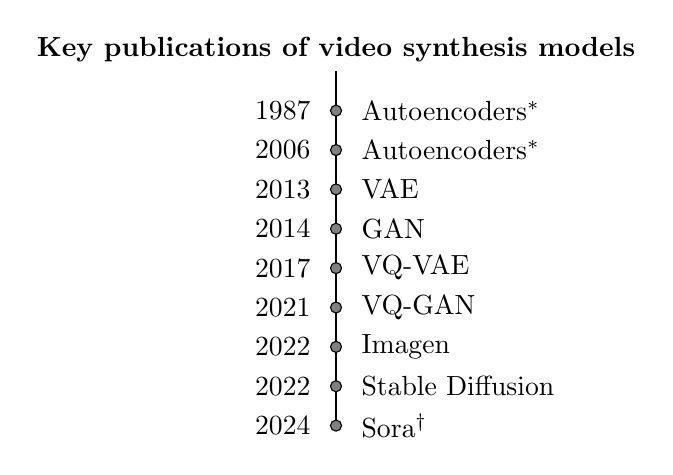
\begin{tikzpicture}
        \def\step{0.5} % step size for vertical spacing
        \def\numtimeline{9} % Number of events in the timeline

        % Define timeline line
        \draw[thick, color=black] (0,0) -- (0,-\numtimeline*\step);

        % Define timeline events with adjusted positions
        \foreach \i/\year/\text in 
        {
            1/1987/Autoencoders$^*$, 
            2/2006/Autoencoders$^*$, 
            3/2013/VAE, 
            4/2014/GAN, 
            5/2017/VQ-VAE,
            6/2021/VQ-GAN,
            7/2022/Imagen,
            8/2022/Stable Diffusion,
            9/2024/Sora$^\dag$
        } {
        \draw[fill=darkgray] (0,-\i*\step) circle (2pt);
        \node[anchor=east] at (-0.2,-\i*\step) {\year};
        \node[anchor=west] at (0.2,-\i*\step) {\text};
        }

        % Define timeline title
        \node[anchor=south] at (0,0) {\textbf{Key publications of video synthesis models}};
    \end{tikzpicture}
    \caption{Chronology of key video generation models publications.}
  \end{figure}

% There are a lot of techniques and models for video generation, and they can be divided into multiple categories:

% \begin{itemize}
%     \item \textbf{Frame prediction}: ...
%     \item \textbf{GAN based models}: such in the case of \cite{chu2020learning} the authors propose 
% \end{itemize}

Video synthesis can be based on four main models and methods:

\begin{enumerate}
    \item \textbf{Diffusion}: diffusion models for video generation extend the iterative refinement process used in image-based diffusion models, such as LDMs, to handle temporal dynamics required for videos. The key idea is to generate not just a sequence of independent images, but a continuous video where both the spatial content of each frame and the temporal coherence between frames are learned and generated simultaneously.
    \item \textbf{Spatial autoregressive}: spatial autoregressive models for video generation, as described in \cite{graves2013generating}, synthesize video by sequentially generating content in a patch-based fashion, where each patch in a frame is conditioned on previously generated patches. This method builds video frame-by-frame, ensuring spatial and temporal coherence across the entire sequence.
    \item \textbf{GAN}: similar to diffusion models, GANs can also be leveraged for video synthesis. 
    \item \textbf{Mask modeling}: mask modeling in video generation uses the technique of selectively masking parts of video frames during training to enhance the model's ability to learn spatial and temporal dependencies. By hiding portions of the video frames, the model is tasked with predicting and reconstructing the missing parts, forcing it to better understand the underlying structure and motion in the video.
\end{enumerate}

\begin{figure}
    \centering
    \includegraphics[width=1\textwidth]{images/video_synthesis/paradigms.png}
    \caption{Overview of video synthesis paradigms \cite{long_video_survey}. Divide and conquer is split into hierarchical architecture for keyframe generation and frame filling. Whereas temporal autoregressive paradigm the next frame prediction depends on the previous frame/frames.}
    \label{fig:video_synthesis_paradigms}
\end{figure}

In the realm of video synthesis there are two paradigms: \textbf{divide and conquer} and \textbf{temporal autoregressive}. An overview of the paradigms is shown in figure \ref{fig:video_synthesis_paradigms}.


\begin{figure}
    \centering
    \includegraphics[width=0.6\textwidth]{images/video_synthesis/generation_technologies.png}
    \caption{An overview of video generation technologies: \textit{GAN:} based on adversarial loss and uses generator and discriminator; \textit{VAE:} compresses the input data in the encoder to lower dimension latent space and then learns to reconstruct the data in the decoder; \textit{Autoregressive:} frame by frame prediction; \textit{Diffusion:} the model adds noise and learns to remove noise with U-Net.}
\end{figure}


\subsection*{Divide and Conquer}

Divide and conquer paradigm breaks the task of video synthesis into smaller, more manageable tasks. This approach can further by divided into 3 methods of approach:

\begin{enumerate}
    \item \textbf{Hierarchical architecture for frame generation}: in this approach, the process is split into \textbf{keyframe generation} and \textbf{frame filling}. Keyframes represent the critical moments of the video that establish the narrative, while the frame-filling models ensure smooth transitions between them. Global models focus on generating the main storyline through keyframes, and local models handle finer details, filling the gaps between the keyframes to maintain temporal consistency.
    \item \textbf{Multi-stage approach for video super-resolution}: \cite{brooks2022generating} suggested generating video by stages, first by creating low-resolution sequences with GAN and then applying super-resolution models to enhance them with StyleGAN3 \cite{stylegan3}.
    % TODO: Explain the combined process of mask modeling, I don't really understand. Maybe read the paper CogVideo?
    \item \textbf{Integrated keyframe and frame filling with mask modeling} simplifies long video generation by combining keyframe creation and frame filling into a unified process. Mask modeling hides specific parts of the video during training, keyframes and intermediate frames simultaneously, like done in CogVideo \cite{cogvideo}, which simplified mask modeling and combines these models into a single model.
\end{enumerate}

\subsection*{Temporal autoregressive}

Temporal autoregressive paradigm is an iterative approach where each frame is generated based on the previous one. The model is trained on sequences of video data, and the output from one timestep serves as the input for the next (the next frame is conditioned on the previous frame, which in theory ensures that the video is temporally coherent).

A significant amount of research has been conducted on temporal autoregressive models, leading to various improvement strategies and enhancements for this framework. Some of the most notable include:

\begin{itemize}
    \item \textbf{Latent space compression}: this method focuses on compressing videos to latent space to optimize computational needs. For example in \cite{zeng2024make} and \cite{gu2023reuse} they explored condensing video data into 3D latent. Compression aims to preserve essential features across dimensions to improve computational efficiency.
    \item \textbf{Incorporating temporal layers} to refine individual video clips. Advancements were made, such as integrating \textbf{temporal layers} (such as attention and convolutional layers) into diffusion models, like in VideoLDM \cite{video_ldm} and \cite{gu2023reuse}. These temporal layers help the model better understand the temporal dynamics of video data.
    \item \textbf{Dual-phase training \& reuse strategies}: dual-training is a training strategy where the model is first trained unconditionally, and then learn to conditionally generate video like in Projected Latent Video Diffusion Model (PVDM) \cite{pvdm}. Given the abundance of unlabeled video data on the web, it's easy to see why this process is attractive. Another method to boost the model's ability to replicate long video sequences is a \textbf{reuse strategy}, which iteratively adds and removes noise during training to simulate natural variability, like in \cite{gu2023reuse}.
\end{itemize}

\subsection*{Spatial autoregressive models}

Spatial autoregressive models are adept at processing tokenized sequence inputs (they include the transformer architecture) which enable the segmentation of video frames into patches. By integrating video data features with the autoregressive power of transformers, these models become more capable of capturing temporal dynamics. In this method, there are two main approaches:

\begin{itemize}
    \item \textbf{Frame tokenization}: like in NUWA-Infinity \cite{nuwa_infinity}, the researchers transform video frames into patches and combine them with spatial positional encodings for more efficient data handling. These autoregressive models, similar to LDMs, compress video data into latent space. Compression techniques like \textbf{Discrete Cosine Transform (DCT)} are used in Transframer \cite{transframer} and by using VQGAN, they convert the frames into latent tokens.
    \item \textbf{Scaling with attention mechanism}: architectural modifications were made by incorporating specialized blocks, such as attention mechanism blocks tailored for spatiotemporal data. For example, Transframer \cite{transframer} integrated temporal and spatial annotations (time-steps, camera viewport, etc.) through cross-attention.
\end{itemize}

\subsection*{Challenges in video synthesis}

Because video synthesis is still developing to this day and is a complex task, there are a lot of open questions to be asked:

\begin{itemize}
    \item How to generate long videos while maintaining high temporal cohesion?
    \item Would it be possible to generate videos in high resolution, with limited computational resources?
    \item How to train video generation models with abundant, unlabeled video data, such as YouTube? Are there any open datasets for video generation?
    \item How to generate videos from text, or other modalities? Is it possible to edit generated videos so it fits our artistic needs?
    \item What is considered a long video? Frame count (e.g., 512, 1024 frames)? Duration (e.g., 3, 5 minutes)?
    \item How we would trade off between resolution (high resolution) of generated video, duration (long), and spatial coherence (smooth motion and logical spatial relationships)? Can we achieve all three?
    \item How to deal with abrupt scene transitions? How to ensure smooth transitions between scenes?
    \item How to measure and evaluate temporal-spatial consistency between video generation models? How to tell if one clip is smoother and more coherent than the other?
\end{itemize}

In \cite{long_video_survey} they surveyed papers in the field of video generation and propose a definition for 'long' videos to exceed 10 seconds long, assuming frame rate of 10fps, or equivalently 100 frames.

\subsection{Evaluation metrics}

\begin{figure}
    \centering
    \includegraphics[width=1\textwidth]{images/video_synthesis/eval_metrics.png}
    \caption{Evaluation metrics in video generation \cite{long_video_survey}.}
    \label{fig:video_synthesis_eval_metrics}
\end{figure}

A common metric used for video generation models is the \textbf{Frechet Video Distance (FVD)} \cite{fvd}, which is an extension of Frechet Inception Distance (FID). FVD compares videos by both spatial and temporal features by using similar process as FID: using a pre-trained 3D ConvNet (i3D), where in FID they use InceptionV3. The i3D network was trained on Kinetics dataset (Kinetics Human Action Video Dataset), and the 3D convolutions capture local and global spatial patterns within the frames. In similar fashion as FID, they compare the distribution of features from generated videos and the FVD is calculated:

\begin{equation*}
    \text{FVD} = \left| \left| \mu_{\text{real}} - \mu_{\text{fake}} \right| \right|^2_2 + \text{Tr} \left( \Sigma_{\text{real}} + \Sigma_{\text{fake}} - 2 \left( \Sigma_{\text{real}} \Sigma_{\text{fake}} \right)^{1/2} \right)
\end{equation*}

The lower the FVD score, the better the video generation model is. A more comprehensive list of evaluation metrics is shown in figure \ref{fig:video_synthesis_eval_metrics}.

Although its not theoretically an evaluation metric, in the Diffusion Transformer (DiT) paper \cite{diffusion_transformer} the researchers used \textbf{Gflops} (giga floating point operations per second) metric to measure the complexity of the model, instead of traditional parameter count of the model. Higher Gflops means the model is more scalable and complex.



\subsection{Previous works}

\begin{figure}
    \centering
    \includegraphics[width=0.7\textwidth]{images/video_synthesis/previous_works.png}
    \caption{Video generation models \& papers \cite{zhou2024survey}.}
\end{figure}

\begin{figure}
    \centering
    \includegraphics[width=1\textwidth]{images/video_synthesis/timeline.png}
    \caption{Text-to-Video generators evolutionary timeline, based on foundational algorithms \cite{sun2024sora}.}
\end{figure}

In \textbf{VideoGAN} \cite{video_gan} (2016) the researchers proposed to use of the large amounts of unlabeled video in order to learn scene dynamics and motion, and capture temporal signals. They proposed a model with \textbf{spatio-temporal convolutional} architecture, and they extend GANs to video generation. They successfully created a video of 1 second long, the model explicitly models the foreground separately from the background, which allows the network to learn which objects are in motion, and which don't. The methodology in this work is autoregressive frame prediction.

In the case of \cite{video_generation_from_text}, where the goal is to generate video from text, they proposed a hybrid model that uses a conditional variational autoencoder (VAE) and a generative adversarial network (GAN). The VAE model will output a 'gist' which is a sketch (intermediate step), how the video will take form (colors, object layout) and the GAN model will apply a set of image filter kernels based on the input text to get an encoded text-gist feature vector and the framework predicts future frames.

\textbf{NUWA-Infinity} \cite{nuwa_infinity} by Microsoft AI (2022) is a text-to-video model that can generate videos in any arbitrary resolution and in any length. Because previous works that use the divide-and-conquer strategy (of using patches to generate image or video) doesn't consider the the dependencies between generated patches explicitly, they struggle to guarantee consistency of generated content. NUWA-Infinity uses the \textbf{autoregressive over autoregressive generation mechanism} that can generate variable-sized videos, in both duration and resolution. This mechanism uses a global patch-level autoregressive
model that considers the dependencies between patches, and a local token-level autoregressive model considers the dependencies between visual tokens within each patch.

\textbf{NUWA-XL} \cite{nuwa_xl} (2023, which is an upgraded version of NUWA-XL) is a diffusion model that uses 3D-UNet for keyframe generation (by global diffusion model) and keyframe filling (by local diffusion model). They also built a new dataset called 'FlintstonesHD' for benchmarking long video generation. Their method reduced inference time when generating 1024 frames from 7.55 minutes to 26 seconds (\textbf{a 94\% reduction in inference time}) on the same hardware.

In \cite{ge2022long} (2022 by Meta AI) they used a conditional (text or images) 3D VQ-GAN with hierarchical transformer architecture to generate long videos (1024 frames or more). They used standard benchmark datasets: UCF-101, Sky Time-lapse and Taichi-HD. They core insight is that using transformers is ideal for capturing long-range temporal dependence.

\textbf{Image-GPT (iGPT):} The OpenAI researchers introduced in a 2020 paper Image-GPT (iGPT) \cite{imagegpt}, in which they tried to explore autoregressive transformer to predict pixels directly, without using CNN prior, only by using the attention mechanism. They pre-trained a transformer on ImageNet and showed that a transformer can learn spatial features (image representation learning). Instead of language tokens, the transformer predicts pixels. The biggest model, called iGPT-XL has 6.8 billion parameters. They also showed that when scaling transformers (more parameters, more pre-training) the architecture quickly closes the gap on contrastive learning of other models that specifically design to this task.

\textbf{VideoGPT} \cite{videogpt} (2021), which we will take a closer look in section \ref{sec:videogpt}, uses VQ-VAE to encode video frames into discrete latent representations by using 3D convolutions and self-attention. It also uses a transformer based on the work of \textbf{Image-GPT} \cite{imagegpt} to generate video frames from the latent representations. VideoGPT uses the same prior networks as Image-GPT.

\textbf{Imagen-Video} \cite{imagen_video} (2022) by Google is a text conditional video generation system based on a cascade of video diffusion models (similar to Imagen (section \ref{sec:imagen})). Instead of 2D super-resolution models as we seen in Imagen, they are spatial and temporal video super-resolution models. Similar to Imagen it also uses frozen T5-XXL \cite{t5_model} text encoder (for text embeddings), it consists of 7 sub-models (1 base model, 3 spatial super-resolution models [SSRs], and 3 temporal super-resolution models [TSRs]) to generate videos of high resolution (1280x768) of 24 frames per second for 5.4 seconds. The diffusion model is 11.6 billion parameters (not including the text encoder). The TSR models increase temporal resolution, whereas SSR increase spatial resolution. The researchers build upon the previous work of \textbf{Video U-Net} architecture \cite{video_diffusion_models}.

\begin{figure}
    \centering
    \includegraphics[width=1\textwidth]{images/video_synthesis/imagen_video.png}
    \caption{Imagen-Video video samples examples.}
\end{figure}

In \textbf{Video Diffusion Models (VDM)} \cite{video_diffusion_models} (2022) by Google proposed a diffusion model for video generation, which is an extension of the standard image diffusion architecture, and can be trained by both images and videos. They proposed to use a \textbf{3D U-Net architecture} in a standard diffusion model to extend to the video domain. They changed the 2D convolution to space-only 3D convolution (if $k$ is the kernel size, then we convert $k\times k$ convolution to $1\times k\times k$), and after each spatial attention block they insert temporal attention block that performs a temporal attention on the first axis. They also use relative position embeddings, similar to positional or time embeddings, so the network can distinguish ordering of video frames.

\textbf{MagicVideo} (2022) \cite{magic_video} from ByteDance (parent company of TikTok) is a text-to-video model leverage LDM based on 3D U-Net and a directed \textbf{temporal attention} (to capture temporal dependencies across frames), and a pre-trained VAE to map video clips to low-dimension latents to learn the distribution of the latent codes. Its based on keyframe and frame filling paradigm and uses CLIP to encode the text prompt.

\textbf{To summarize}, there is a common consensus among the researchers in the previous works. They agree that in order to generate high-cohesion long videos, we need to model long-range temporal dependence in videos with many more frames. Not only that, but also that base models GANs are difficult to optimize for video generation tasks because of the adversarial loss, unlike the likelihood loss found in every other base model (VAE, diffusion, transformers). And finally, they agree that \textit{"the video domain has not yet witnessed its 'AlexNet moment'"} [quote from \cite{tran2018closer}] (AlexNet \cite{alexnet} was a major breakthrough in 2012 for image classification task which led to the development of imaging domain in deep learning). 






\subsection{Spatiotemporal feature learning}

One of the first work that tries to capture temporal dynamics is in a form of sequence-to-sequence video captioning \cite{venugopalan2015sequence} (2015). In this paper, the researchers used \textbf{Long Short-Term Memory model (LSTM)} to caption video, which was a popular model for sequence tasks at that time (and also Recurrent Neural Networks [RNN] which was prior work to LSTMs). However LSTM falls short in capturing long-range dependencies, and among other problems (like deep LSTM has training problems because of the exploding/vanishing gradient problem, difficult scaling and more), was quickly replaced by other models.

Since then, 3D convolution (explained below) and vision transformers (appendix \ref{appendix:vision_transformer}) have overtaken LSTM and RNN approaches for local, global attention in vision tasks.

\begin{figure}
    \centering
    \includegraphics[width=1\textwidth]{images/video_synthesis/conv.png}
    \caption{2D and 3D convolution operations. (a) Applying 2D convolution on image results in an image. (b) Applying 2D convolution on video (multiple frames) also results in an image. (c) Applying 3D convolution on video results in another volume (channel), preserving temporal information. Figure from the 2014 paper \cite{tran2015learning}.}
\end{figure}

A 2014 paper \cite{tran2015learning} by Facebook AI suggested using 3D-ConvNets (3D convolution networks) for video data spatiotemporal feature learning. The dataset that they used are UCF101, Sports-1M, and because Sports-1M has 100x times the amount of video clips compared to UCF101. For each video clip, they extracted five 2-second clips as the train-test split and resized the frames to 128x171, and flipped the frames horizontally with 50\% probability.

Compared to 2D ConvNet, 3D ConvNet has the ability to model temporal information better owing to 3D convolution and 3D pooling operations. The researchers found that 3x3x3 kernel size is the best option for 3D ConvNets. After every 3D convolution layer they apply 3D max-pooling.

\begin{figure}
    \centering
    \includegraphics[width=1\textwidth]{images/video_synthesis/c3d_feature_maps.png}
    \caption{Feature maps of the first 3D convolution layer of the C3D model \cite{tran2015learning}. The first two rows of the feature maps shows the detection of moving edges and blobs, while the last row shows edge orientation changes and color changes.}
    \label{fig:c3d_feature_maps}
\end{figure}

Figure \ref{fig:c3d_feature_maps} shows the feature maps of the first 3D convolution layer of the C3D model. The 3D convolution helps to capture motion between frames.

In a 2018 paper \cite{tran2018closer} that reviews spatiotemporal convolution (also by Facebook AI), they observed that 2D CNNs applied on individual frames of video remain solid performers in action recognition (the classification of action [like cooking, running, dancing] in image/video). By using residual connections, and by factorizing the 3D convolutional filters into separate spatial and temporal components results in the creation of a new spatiotemporal convolution block called \texttt{R(2+1)D}. The \texttt{R(2+1)D} block is a 2D residual block followed by a 1D temporal convolution. This separation allows the model to represent more complex non-linear functions, and is more easily optimized.







\subsection{Practices \& techniques in vision domain}

\begin{figure}
    \centering
    \includegraphics[width=1\textwidth]{images/video_synthesis/spatial_and_temporal_self_attention.png}
    \caption{Spatial and temporal self-attention topology graph illustration \cite{plizzari2021spatial}. The model tries to learn 3D skeleton pose over time. \textit{Left:} full-graph of skeleton joins; spatial self-attention (SSA): the model learns the relations between joints (nodes). \textit{Right:} temporal self-attention (TSA); the dynamics of each joint is studied separately along all the frames, each node is independent and correlations between frames are computed between the same body joints along the temporal dimension.}
    \label{fig:spatial_temporal_self_attention}
\end{figure}

In this section we explore common practices or techniques used in vision domain, that are applied in image synthesis and video synthesis models.

\textbf{Use of Transformers for Multi-modal outputs:} Transformers have been shown time and time again their capability to scale to very large models. In addition, they excel at sequence-to-sequence tasks, which allows researchers to use them in their vision models and condition on multiple types of data (text, audio, image, layouts, semantic masks, etc). As we advance further into more and more advanced vision models, we see increase in the use of transformers in vision tasks.

\textbf{Patchify:} In Vision Transformer (ViT) \cite{vision_transformer} (appendix \ref{appendix:vision_transformer}) and Diffusion Transformer (DiT) \cite{diffusion_transformer} (appendix \ref{appendix:diffusion_transformer}) both use patch technique to model and represent patches of size $p \times p$ of an image. First the image is divided into patches, then each patch is linearly embedded into a vector, and the position (either absolute, relative or even distance between patches) of the patch is added (element-wise) to the patch embeddings, forming an embedding of patch + position tokens, and then the sequence of tokens is fed into the transformer (in the case of ViT and DiT). 

\textbf{Spatial Self-Attention (SSA):} Self-attention mechanism is often used to capture long-range spatial dependencies in a single frame. Unlike CNNs, which capture only local features, self-attention allows the model to learn the global of an image. Spatial self-attention is used in Vision Transformer (ViT) \cite{vision_transformer} (appendix \ref{appendix:vision_transformer}), for instance.

\textbf{Temporal Self-Attention (TSA):} Self-attention mechanism is also often used to capture temporal dependencies (relationships between frames). For example, it enables the model to understand how each part of the video changes over time, allowing it to learn motion patterns. Video-LDM \cite{video_ldm} (section \ref{sec:videoldm}) for example uses temporal self-attention.

\textbf{Color reduction:} In \cite{imagegpt} they proposed context reduction: first by downsizing the resolution of the training videos to lower resolution, and more importantly, they created their own 9-bit color palette by K-mean clustering (k=512). That means, each pixel is represented by 9 bits, instead of 256x256x256 (which require 8+8+8=24 bits). This color reduction yields a sequence length three times shorter than the standard (R, G, B) palette.

\textbf{Use of compute efficient attention blocks:} Like in the case of Video-GPT they use \textbf{Axial attention} block (appendix \ref{appendix:attention}), which doesn't compute self-attention of the entire image, but only of the rows and columns separately. This reduces the complexity of the attention mechanism.

\textbf{Operating in latent space:} Because video synthesis is compute intensive task, a lot of previous works models operate in latent space, which is compressed lower-dimension space, compared to raw RGB frames. Most of the time, variational autoencoder is used to encode to latent space and the decoder to decode the latent space back to the RGB space.

\textbf{Conditioning:} There are three ways to condition an image/video generation model: \textbf{cross-attention} which we saw in stable diffusion, \textbf{adaptive layer normalization} (like in diffusion transformer) and in transformer-based models, the conditional information is added to the \textbf{input sequence tokens} (like in ViT and DiT) to be fed into the transformer decoder.



% Previous works
\section{VideoGPT}
\label{sec:videogpt}

VideoGPT \cite{videogpt} uses likelihood based VQ-VAE model and a transformer model based on the GPT architecture. The encoder of VQ-VAE first downsamples video into discrete latent space using 3D convolutions, and then the decoder reconstructs the video from these latent codes.

\subsection*{The VQ-VAE}

Reminder that the loss function of VQ-VAE is defined as:

\begin{equation*}
    \mathcal{L} = \underbrace{\left| \left| x - D(e) \right| \right|^2_2}_{\mathcal{L}_\text{recon}} + \underbrace{\left| \left| \text{sg}\left[ E(x) \right] - e \right| \right|^2_2}_{\mathcal{L}_\text{codebook}} + \underbrace{\beta \left| \left| \text{sg}[e] - E(x) \right| \right|^2_2}_{\mathcal{L}_\text{commit}}
\end{equation*}

where $\text{sg}$ refers to stop-gradient, $\mathcal{L}_\text{recon}$ is the \textbf{reconstruction loss} (encourages the VQ-VAE to learn good representations to accurately reconstruct the data), $\mathcal{L}_\text{codebook}$ is the \textbf{codebook loss} (quantization loss, it brings codebook vectors closer to the encoder outputs), and $\mathcal{L}_\text{commit}$ is the \textbf{commitment loss} (which prevents the encoder outputs from fluctuating between different code vectors). 

The reconstruction loss optimizes only the decoder, the commitment loss optimizes only the encoder, and the codebook loss optimizes the codebook embeddings only. See section \ref{vqvae} for more details.

The researchers used EMA (exponential moving average which is described in the VQ-VAE paper \cite{vqvae}) update for the codebook loss. In short, it makes the VQ-VAE faster to train and converge.

\begin{figure}
    \centering
    \includegraphics[width=0.5\textwidth]{images/video_gpt/res_atten_block.png}
    \caption{Residual attention block as described in VideoGPT \cite{videogpt} which are used in the VQ-VAE model \cite{videogpt}.}
    \label{fig:videogpt_res_atten_block}
\end{figure}

To train the VQ-VAE model (to learn the latent codes), the authors trained the VQ-VAE on video data. The encoder consists of a downsample 3D convolutions followed by attention residual blocks (figure \ref{fig:videogpt_res_atten_block}), and \texttt{LayerNorm}. The \texttt{LayerNorm} layers are described in appendix \ref{appendix:blocks_norm}. The position embeddings is not explained in the paper; but we can infer them as the frame position (i.e. frame 0, 1, ... in the video), which is added element-wise.

The architecture of the decoder is the reverse of the encoder (residual attention blocks followed by upscale 3D convolutions).








\subsection*{The transformer (GPT)}

GPT is autoregressive transformer architecture (appendix \ref{appendix:transformers}). The autoregressive nature can be described as:

\[ p(x) = \prod_{i=1}^{d} p(x_i | x_{\leq i}) \] 

through masked self-attention. The GPT transformer is optimized using maximum likelihood (appendix \ref{appendix:likelihood_function}). The transformer follows the same prior networks as Image-GPT \cite{imagegpt}.

In \textbf{Image-GPT} the network learns to predict pixels and only a transformer is used, which is the first time a transformer-only image synthesis model was proposed (no CNN prior!). The model learns to predict pixels autoregressively based on a probability distribution modeled on each of the previous pixels. The attention mechanism helps in the modeling of the spatial pixel features. The iGPT-XL model consists of 6.8 billion parameters, iGPT-M has 455 million parameters, and iGPT-S has 76 million parameters. The researchers wanted to test how generative pre-training can be useful to learn image representations in large scale.










\subsection{Architecture}

\begin{figure}
    \centering
    \includegraphics[width=0.6\textwidth]{images/video_gpt/architecture.png}
    \caption{VideoGPT architecture \cite{videogpt}. Left: training the VQ-VAE; Right: training the autoregressive transformer model on the latent vectors \cite{videogpt}.}
    \label{fig:videogpt_architecture}
\end{figure}

The architecture of VideoGPT is shown in figure \ref{fig:videogpt_architecture}.

\textbf{VQ-VAE:} They train the VQ-VAE on video data to learn the codebook. The encoder and decoder consists of 3D convolutions (appendix \ref{appendix:blocks_3dconv}) followed by attention residual blocks (figure \ref{fig:videogpt_res_atten_block}). Axial attention \cite{axial_attention} block is described in appendix \ref{appendix:attention}. The purpose of the VQ-VAE is to encode the video into discrete latent space. The purpose of the transformer is to autoregressively generate the video from these latents.

\textbf{Transformer:} The right side of figure \ref{fig:videogpt_architecture} shows the training of the autoregressive transformer model on the latent vectors. \textbf{The target is the next latent code (frame) in the video}. So the transformer learns to predict the next frame as a latent code.






\subsection{Video generation}

\begin{figure}
    \centering
    \includegraphics[width=0.8\textwidth]{images/video_gpt/video_generation.png}
    \caption{Video samples from VideoGPT \cite{videogpt}.}
    \label{fig:videogpt_video_generation}
\end{figure}

The model can start to autoregressively generate videos given starting image: the VQ-VAE turns the first image to latent vector, and this vector is then fed to the GPT transformer to generate the next frame. The process is repeated until the desired number of frames is generated.

Multiple video generation examples are shown in figure \ref{fig:videogpt_video_generation}.



% \section{Sora}

% TODO: Add more
Sora by OpenAI is a video synthesis model, if not one of the best video synthesis models to date. It was introduced in a 2023 paper \cite{sora}. The model is based on the principles of Stable Diffusion, Video-LDM and DiT. They leverage the scalability of the transformer architecture in DiT and use their already pre-trained GPT-4o model as the backbone (\cite{sun2024sora} section 3.1.2). The innovation in Sora is the use of diffusion, working in latent space, replacing U-Net with transformers, and the use of both adaptive layer norm and cross-attention for text conditioning.



% Main works
\section{Video-LDM}
\label{sec:videoldm}

Video-LDM (2023) by NVIDIA \cite{video_ldm} is a T2V model based on LDM. It first trains an image generator on image datasets, then freeze the layers, and then adds temporal layers which helps to align images in temporally consistent manner, transforming it from T2I model to T2V model. Then the model is fine-tuned on video dataset. Freezing the spatial layers transforms the image generation knowledge to the video domain. The model achieves high resolutions of up to $1280\times 2048$.


\subsection*{Mathematical notations}

The LDMs autoencoder compresses the high-dimensional input data $x \in \mathbb{R}^{T \times 3 \times \hat{H} \times \hat{W}}$ where $x \sim p_{\text{data}}$ is a sequence of $T$ RGB frames with height $\hat{H}$ and width $\hat{W}$ to lower-dimensional latent space $z = \mathcal{E} (x) \in \mathbb{R}^{T \times C \times H \times W}$ (where $C$ is the number of latent channels, and $H, W$ are the spatial latent dimensions). The model then learns to reconstruct $x$ with the decoder $\mathcal{D}$: $\hat{x} = \mathcal{D} (\mathcal{E} (x)) \sim x$.

Let us denote the spatial layers $l^i_{\theta}$ where $\theta$ are the model's parameters, and $i$ is the layer index. We then denote the addition of temporal layers as $l^i_{\phi}$ to learn to align individual frames in a temporally consistent manner. We denote $f_{\theta, \phi}$ as the full model (with spatial and temporal layers).








\subsection{Architecture}

\begin{figure}
    \centering
    \includegraphics[width=0.7\textwidth]{images/video_ldm/stack.png}
    \caption{Video-LDM stack \cite{video_ldm}. (1) Keyframe generation. (2) Keyframe filling (keyframe interpolation). (3) Keyframe interpolation is repeated a second time. (4) The latents are decoded to pixel space. (5) Optionally, SR model is applied \cite{video_ldm}.}
    \label{fig:video_ldm_stack}
\end{figure}

The architecture of Video-LDM is similar to Stable Diffusion except for the added temporal layers, and the addition of autoencoder for latent encoding/decoding and the discriminator which helps photorealism in the decoder network. The model's stack is shown in figure \ref{fig:video_ldm_stack}.

\begin{figure}
    \centering
    \includegraphics[width=0.6\textwidth]{images/video_ldm/ddpm_sde.png}
    \caption{Generative modeling through stochastic differential equations (SDE) \cite{song2020score}.}
    \label{fig:video_ldm_ode}
\end{figure}

Figure \ref{fig:video_ldm_ode} illustrates the stochastic diffusion process, showing SDE paths that represent sample trajectories. Data distribution $p(x)$ transitions to prior distribution $p_T(x)$ via forward SDE (adding noise) and reverses back to $p(x)$ using reverse SDE. As noise is added, structured data becomes progressively chaotic, converging to a Gaussian prior before reverting to the original distribution. The distribution depicts the data probability, the middle distribution depicts the Gaussian prior, and the right distributions depicts reconstructed data.

\begin{figure}
    \centering
    \includegraphics[width=0.8\textwidth]{images/video_ldm/image_to_video_tuning.png}
    \caption{Transforming image LDM (left) to video LDM (right) via temporal fine-tuning \cite{video_ldm}.}
    \label{fig:video_ldm_image_to_video_tuning}
\end{figure}

In figure \ref{fig:video_ldm_image_to_video_tuning} we see the temporal fine-tuning. We see the stochastic denoising process of diffusion, similar to figure \ref{fig:video_ldm_ode}. We can see that the images on the left side are not temporally aligned, whereas on the right, the images form a coherent video.

\begin{figure}
    \centering
    \includegraphics[width=0.6\textwidth]{images/video_ldm/enc_dec_denoise_process.png}
    \caption{\textit{Top}: frozen encoder \textit{Right}:  \textit{Bottom}: generative denoising process. \cite{video_ldm}}
    \label{fig:video_ldm_enc_dec_denoise_process}
\end{figure}

In figure \ref{fig:video_ldm_enc_dec_denoise_process} we can see the frozen encoder compresses video frames into 3D latents and the decoder learns to reconstruct them. On the right, we can see the patch-based discriminator $\mathcal{H}$ which is used to increase photorealism of the decoder. It is trained on the adversarial objective which is added to the AE reconstruction score like in PatchGAN \cite{isola2017image} (which tries to classify if $N \times N$ patch is real or fake). On the bottom we can see the generative denoising process, where each embedding corresponds to different image latent in the decoder $\mathcal{D}$.

\begin{figure}
    \centering
    \includegraphics[width=1\textwidth]{images/video_ldm/temporal_layers.png}
    \caption{The researchers turn pre-trained LDM (in gray) into video generator by adding temporal layers (in green) \cite{video_ldm}.}
    \label{fig:video_ldm_spatial_temporal_mixing_layers}
\end{figure}

In figure \ref{fig:video_ldm_spatial_temporal_mixing_layers} we can see that the pre-trained LDM (in gray) is turned into a video generator (on the right) by adding temporal layers $l_\phi$ (in green) that learn to align images in a temporally consistent manner. The spatial layers $l_\theta$ are frozen (in gray) and only the temporal layers are learned (in green). On the right we can see closer look of spatial, temporal layers. One problem arises, though. The pre-trained LDM is trained only on batch, channel, height and width dimensions, but video has one additional dimension: the temporal $t$ dimension. So, in order to deal with the addition of the temporal dimension, they \textbf{rearranged the batch dimension} to be mixed with the temporal dimension (instead of $b$ the batch dimension is now $(b\ t)$) for the next layer: $(b\ t)\ c\ h\ w \rightarrow b\ t\ c\ h\ w$. The $c_S$ represents a context vector used for conditioning the model (explained below in subsection \textbf{context guidance \& masking}).

The input of the spatial layers $l_\theta^i$ is of the dimension $b\ c\ h\ w$ whereas the input dimension of temporal layers is of the dimension $b\ t\ c\ h\ w$. This notation is called \texttt{Einops} (einstein operations) and is further discussed in the Einops paper \cite{einops}. The spatial layers interpret the video as a batch of images by shifting the temporal axis into the batch dimension (the spatial layers treat all $B \cdot T$ encoded video frames in the batch dimension $b$). It is important to note that the rearrange operation doesn't change the tensor values; rather it rearranges the dimensions.

For the 3D convolution (temporal layer), they reshape the input back to video dimensions (they process entire videos in new temporal dimension $t$): 

\[ \underbrace{(b\ t)\ c\ h\ w}_{\text{Output of spatial layer}} \rightarrow \underbrace{b\ c\ t\ h\ w}_{\text{Input to the next Conv3D layer}} \]

After the temporal layers they reshape the input back to fit into the spatial layers like so:

\[ \underbrace{b\ c\ t\ h\ w}_{\text{Output of Conv3D layer}} \rightarrow \underbrace{(b\ t)\ c\ h\ w}_{\text{Input to the next spatial layer}} \]

As for the temporal attention layer (temporal layer), they reshaped the input back to work on the temporal dimension, instead of spatial:

\[ \underbrace{(b\ t)\ c\ h\ w}_{\text{Output of spatial layer}} \rightarrow \underbrace{(b\ h\ w) \ t\ c}_{\text{Input to the next temporal attention layer}} \]

\[ \underbrace{(b\ h\ w) \ t\ c}_{\text{Output of temporal attention layer}} \rightarrow \underbrace{(b\ t)\ c\ h\ w}_{\text{Input to the next spatial layer}} \]

\begin{figure}
    \centering

    \begin{subfigure}{0.3\textwidth}
        \centering
        \scalebox{0.5}{
            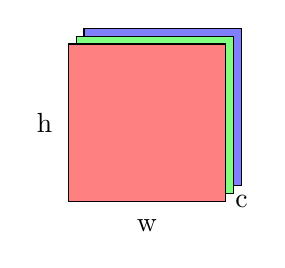
\begin{tikzpicture}
    % Blue channel slice
    \draw[fill=blue!50] (0, 0) rectangle (2, 2);

    % Green channel slice
    \draw[fill=green!50] (-0.1, -0.1) rectangle (1.9, 1.9);
    
    % Red channel slice
    \draw[fill=red!50] (-0.2, -0.2) rectangle (1.8, 1.8);

    \node at (0.8, -0.5) {w};
    \node at (-0.5, 0.8) {h};
    \node at (2, -0.2) {c};
    
\end{tikzpicture}

        }
        \caption{A single frame. The $c\ h\ w$ dimensions.}
    \end{subfigure}

    \begin{subfigure}{0.3\textwidth}
        \centering
        \scalebox{0.5}{
            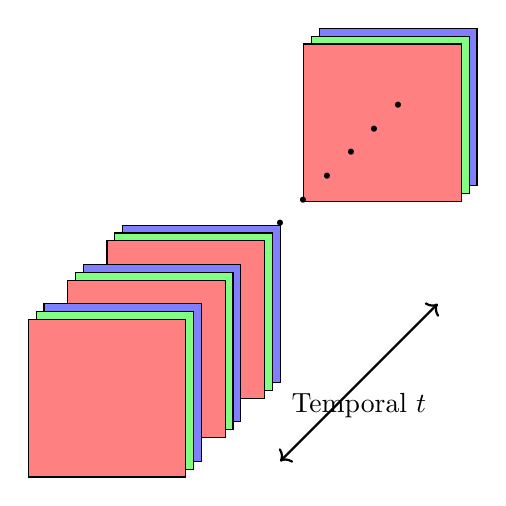
\begin{tikzpicture}
    \def\width{2}
    \def\height{2}
    \def\shift{0.1} % Shift for the green and red channels

    \def\xshift{-0.5}  % Shift in the x direction for duplication
    \def\yshift{-0.5}  % Shift in the y direction for duplication
    \def\lastrectxshift{\xshift * -5} % Last image should be shifted more because of three dots
    \def\lastrectyshift{\yshift * -5} % Last image should be shifted more because of three dots
    \def\dotstartx{2}  % Starting x position for the dots
    \def\dotstarty{2}  % Starting y position for the dots
    \def\dotshift{0.3}  % Shift for the dots


    % First rectangle
    \draw[fill=blue!50] (0, 0) rectangle (\width, \height);
    \draw[fill=green!50] (-\shift, -\shift) rectangle (\width-\shift, \height-\shift);
    \draw[fill=red!50] (-2*\shift, -2*\shift) rectangle (\width-2*\shift, \height-2*\shift);

    % Second rectangle
    \draw[fill=blue!50] (\xshift, \yshift) rectangle (\xshift+\width, \yshift+\height);
    \draw[fill=green!50] (\xshift-\shift, \yshift-\shift) rectangle (\xshift+\width-\shift, \yshift+\height-\shift);
    \draw[fill=red!50] (\xshift-2*\shift, \yshift-2*\shift) rectangle (\xshift+\width-2*\shift, \yshift+\height-2*\shift);

    % Third rectangle
    \draw[fill=blue!50] (2*\xshift, 2*\yshift) rectangle (2*\xshift+\width, 2*\yshift+\height);
    \draw[fill=green!50] (2*\xshift-\shift, 2*\yshift-\shift) rectangle (2*\xshift+\width-\shift, 2*\yshift+\height-\shift);
    \draw[fill=red!50] (2*\xshift-2*\shift, 2*\yshift-2*\shift) rectangle (2*\xshift+\width-2*\shift, 2*\yshift+\height-2*\shift);

    % Fourth rectangle
    \draw[fill=blue!50] (\lastrectxshift, \lastrectyshift) rectangle (\lastrectxshift+\width, \lastrectyshift+\height);
    \draw[fill=green!50] (\lastrectxshift-\shift, \lastrectyshift-\shift) rectangle (\lastrectxshift+\width-\shift, \lastrectyshift+\height-\shift);
    \draw[fill=red!50] (\lastrectxshift-2*\shift, \lastrectyshift-2*\shift) rectangle (\lastrectxshift+\width-2*\shift, \lastrectyshift+\height-2*\shift);


    % Dots
    \node at (\dotstartx, \dotstarty) {\huge$\cdot$};
    \node at (\dotstartx + \dotshift, \dotstarty + \dotshift) {\huge$\cdot$};
    \node at (\dotstartx + \dotshift*2, \dotstarty + 2*\dotshift) {\huge$\cdot$};
    \node at (\dotstartx + \dotshift*3, \dotstarty + 3*\dotshift) {\huge$\cdot$};
    \node at (\dotstartx + \dotshift*4, \dotstarty + 4*\dotshift) {\huge$\cdot$};
    \node at (\dotstartx + \dotshift*5, \dotstarty + 5*\dotshift) {\huge$\cdot$};

    % Arrow
    \draw[<->, thick] (2, -1) -- (4, 1) node[midway, below] {Temporal $t$};

    

\end{tikzpicture}

        }
        \caption{Multiple frames. The $t\ c\ h\ w$ dimensions.}
    \end{subfigure}

    \begin{subfigure}{0.7\textwidth}
        \centering
        \scalebox{0.5}{
            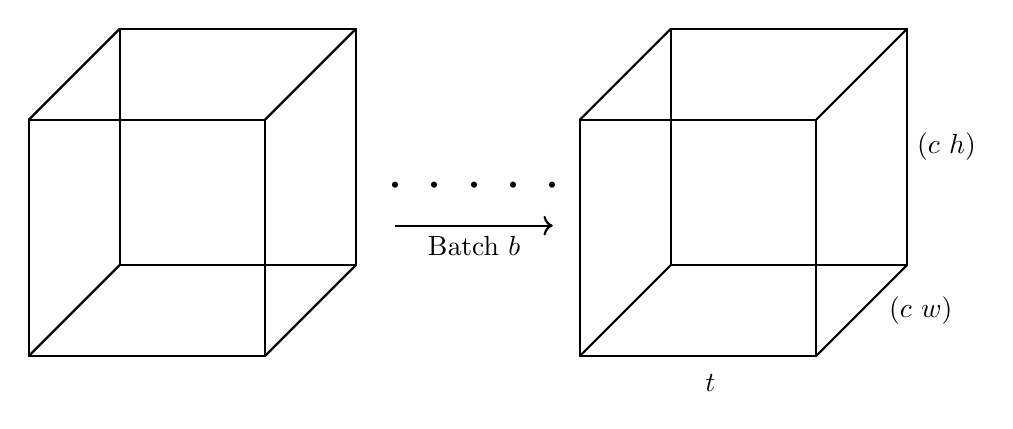
\begin{tikzpicture}
    % First cube
        % variables
        \def\cubeWidth{3}
        \def\cubeHeight{3}
        \def\cubeDepth{3}
    
        % Cube points
        \coordinate (A) at (0, 0, 0);
        \coordinate (B) at (\cubeWidth, 0, 0);
        \coordinate (C) at (\cubeWidth, \cubeHeight, 0);
        \coordinate (D) at (0, \cubeHeight, 0);
        \coordinate (E) at (0, 0, \cubeDepth);
        \coordinate (F) at (\cubeWidth, 0, \cubeDepth);
        \coordinate (G) at (\cubeWidth, \cubeHeight, \cubeDepth);
        \coordinate (H) at (0, \cubeHeight, \cubeDepth);
    
        % Draw cube
        \draw[thick] (A) -- (B) -- (C) -- (D) -- cycle;
        \draw[thick] (E) -- (F) -- (G) -- (H) -- cycle;
        \draw[thick] (A) -- (E);
        \draw[thick] (B) -- (F);
        \draw[thick] (C) -- (G);
        \draw[thick] (D) -- (H);
    
        % Axes
        \node at (0.5, -1.5, 0) {$t$};
        \node at (\cubeWidth + 0.5, \cubeHeight/2, 0) {$(c\ h)$};
        \node at (\cubeWidth + 0.75, 0, \cubeDepth/2) {$(c\ w)$};

    % Second cube
        % variables
        \def\cubeShiftX{-7}
        \def\cubeShiftY{0}
    
        % Cube points (shifted)
        \coordinate (A') at (\cubeShiftX, \cubeShiftY, 0);
        \coordinate (B') at (\cubeShiftX + \cubeWidth, \cubeShiftY, 0);
        \coordinate (C') at (\cubeShiftX + \cubeWidth, \cubeShiftY + \cubeHeight, 0);
        \coordinate (D') at (\cubeShiftX, \cubeShiftY + \cubeHeight, 0);
        \coordinate (E') at (\cubeShiftX, \cubeShiftY, \cubeDepth);
        \coordinate (F') at (\cubeShiftX + \cubeWidth, \cubeShiftY, \cubeDepth);
        \coordinate (G') at (\cubeShiftX + \cubeWidth, \cubeShiftY + \cubeHeight, \cubeDepth);
        \coordinate (H') at (\cubeShiftX, \cubeShiftY + \cubeHeight, \cubeDepth);
    
        % Draw the second cube
        \draw[thick] (A') -- (B') -- (C') -- (D') -- cycle;
        \draw[thick] (E') -- (F') -- (G') -- (H') -- cycle;
        \draw[thick] (A') -- (E');
        \draw[thick] (B') -- (F');
        \draw[thick] (C') -- (G');
        \draw[thick] (D') -- (H');

    % Three dots
        % variables
        \def\dotStartX{-3.5}
        \def\dotStartY{1}
        \def\dotShiftX{0.5}
        \def\dotShiftY{0}
    
        % dots
        \node at (\dotStartX, \dotStartY) {\huge$\cdot$};
        \node at (\dotStartX + \dotShiftX, \dotStartY + \dotShiftY) {\huge$\cdot$};
        \node at (\dotStartX + \dotShiftX * 2, \dotStartY + \dotShiftY * 2) {\huge$\cdot$};
        \node at (\dotStartX + \dotShiftX * 3, \dotStartY + \dotShiftY * 3) {\huge$\cdot$};
        \node at (\dotStartX + \dotShiftX * 4, \dotStartY + \dotShiftY * 4) {\huge$\cdot$};


    % Arrow
    \draw[->, thick] (-3.5, 0.5) -- (-1.5, 0.5) node[midway, below] {Batch $b$};
\end{tikzpicture}
        }
        \caption{All the $b\ t\ c\ h\ w$ dimensions.}
    \end{subfigure}

    \caption{Representation of video dimensions $b\ t\ c\ h\ w$ which corresponds to batch, temporal, channel, height, width dimensions.}
    \label{fig:video_ldm_dimensions}
\end{figure}

We can see visual representation of the dimensions (batch, temporal, channel, height, width) in figure \ref{fig:video_ldm_dimensions}. It's made clear what each dimension represents in the video data.



\textbf{Mixing factor}: after each temporal layer, the output $z'$ is combined with the output of previous spatial layer output $z$ to form a mixing: 

\[ \underbrace{\alpha_\phi^i z_{i} + (1 - \alpha_\phi^i) z_{i}'}_{\text{Mixing factor}} \] 

where $\alpha_\phi^i \in [0, 1]$ and is a learnable parameter. If we set $\alpha = 1$ for each layer skip the temporal score, and we retain the native image generation capability. This mixing operation is similar to CFG (mixing between conditional score and unconditional score).

\textbf{Temporal mixing layers}: two types of temporal mixing layers in use (see figure \ref{fig:video_ldm_spatial_temporal_mixing_layers}) are the \textit{temporal attention} and \textit{Conv3D} layer.

\textbf{Noise scheduler}: Video-LDM uses the same noise scheduler as the underlying image model. In table 6 of the paper, it shows that in all of their models, they use linear noise scheduler.

\textbf{Training objective}: in the training phase only the temporal layers are trained. The objective is the LDM objective (likelihood based, predicting noise in U-Net):

\[ \arg \min_\phi \mathbb{E}_{x \sim p_{\text{data}}, \tau \sim p_{\tau}, \epsilon \sim \mathcal{N} (0, I)} \left[ \left| \left| y - f_{\theta,\phi} (z_{\tau} ; c, \tau) \right| \right|^2_2 \right] \]

where $\tau$ is the diffusion time step, $y$ is the target noise vector. The target is to minimize the difference between predicted noise and ground truth $y$ over all video frames.

\textbf{Adding temporal layers to the decoder:} the researchers add temporal layers to the decoder of the AE which they found this step to be critical for achieving good results. The reason is that the AE is trained on images and flickering artifacts are present in the generated videos (because training on images doesn't teach the model temporal dynamics). So the researchers fine-tune the decoder on video data with a \textbf{patch-wise temporal discriminator built from 3D convolutions}. The encoder, however, remains unchanged.

\textbf{Patch-wise temporal discriminator:} The patch-wise temporal discriminator $\mathcal{H}$, which is built from 3D convolutions, is used to fine-tune the decoder. It's trained on video data and returns "real" or "fake" prediction on patches of the video clip.


\begin{figure}
    \centering
    \scalebox{0.4}{
        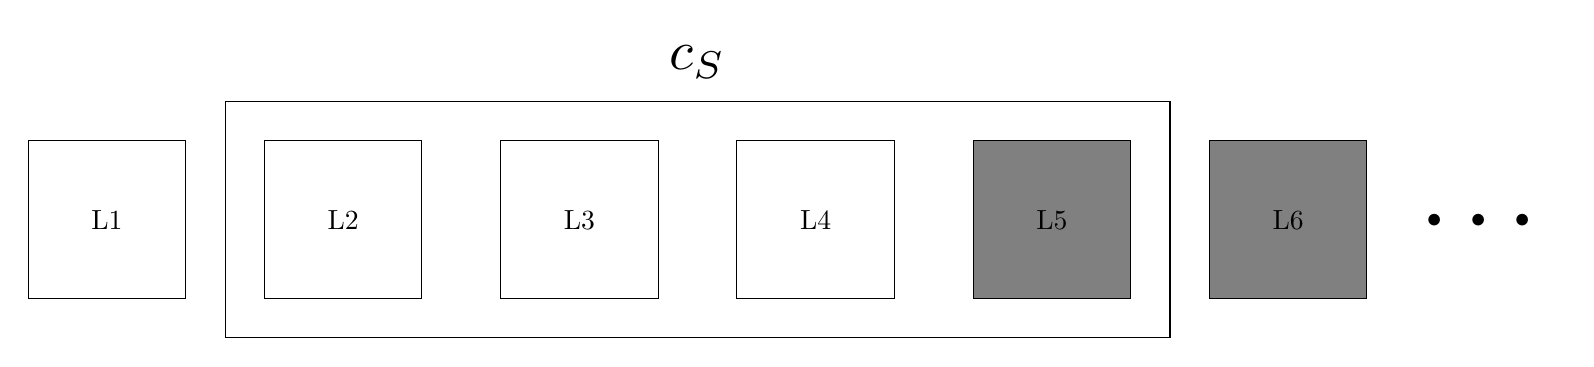
\begin{tikzpicture}
    \draw[fill=white!50] (0, 0) rectangle (2, 2);
    \node[anchor=center] at (1, 1) {L1};

    \draw[fill=white!50] (3, 0) rectangle (5, 2);
    \node[anchor=center] at (4, 1) {L2};

    \draw[fill=white!50] (6, 0) rectangle (8, 2);
    \node[anchor=center] at (7, 1) {L3};

    \draw[fill=white!50] (9, 0) rectangle (11, 2);
    \node[anchor=center] at (10, 1) {L4};

    \draw[fill=black!50] (12, 0) rectangle (14, 2);
    \node[anchor=center] at (13, 1) {L5};

    \draw[fill=black!50] (15, 0) rectangle (17, 2);
    \node[anchor=center] at (16, 1) {L6};

    % c_S
    \node[anchor=center, scale=2] at (8.5,3) {$c_S$};

    % Context guidance box
    \draw[] (2.5, -0.5) rectangle (14.5, 2.5);

    % 3 Dots
    \node [scale=4] at (18,1) {\rotatebox{90}{$\vdots$}};
\end{tikzpicture}
    }
    \caption{Keyframe model learns to predict the next latent frame $z$ by context guidance (conditioned on previous frames).}
    \label{fig:video_ldm_keyframes}
\end{figure}

\begin{figure}
    \centering
    \scalebox{0.4}{
        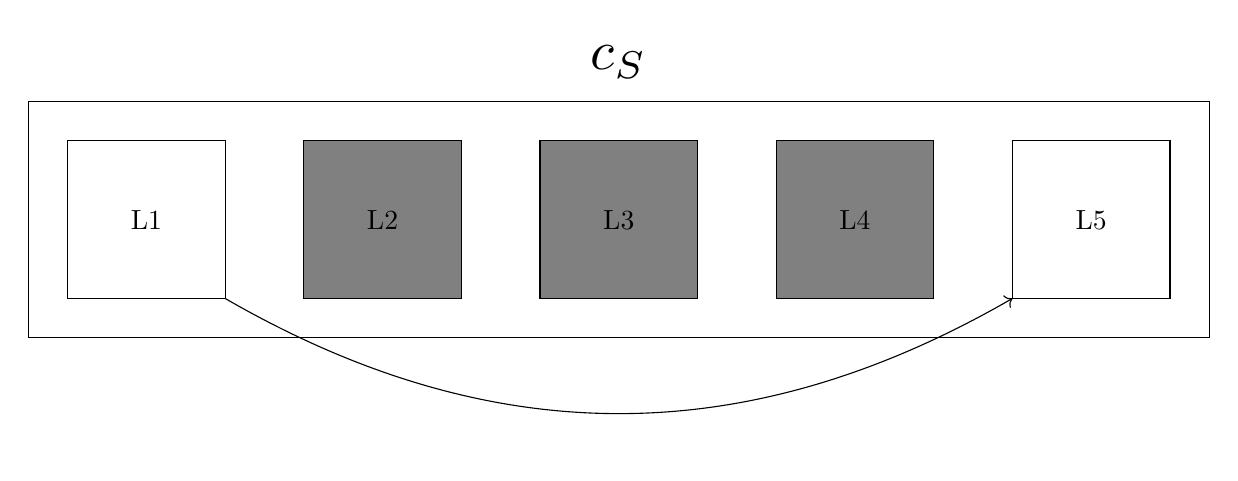
\begin{tikzpicture}
    \draw[fill=white!50] (0, 0) rectangle (2, 2);
    \node[anchor=center] at (1, 1) {L1};

    \draw[fill=black!50] (3, 0) rectangle (5, 2);
    \node[anchor=center] at (4, 1) {L2};

    \draw[fill=black!50] (6, 0) rectangle (8, 2);
    \node[anchor=center] at (7, 1) {L3};

    \draw[fill=black!50] (9, 0) rectangle (11, 2);
    \node[anchor=center] at (10, 1) {L4};

    \draw[fill=white!50] (12, 0) rectangle (14, 2);
    \node[anchor=center] at (13, 1) {L5};

    \draw[->] (2, 0) to[bend right] (12, 0);

    \node[anchor=center, scale=2] at (7,3) {$c_S$};
    \draw[] (-0.5, -0.5) rectangle (14.5, 2.5);
\end{tikzpicture}
    }
    \caption{Interpolation model learns to fill masked latents $m \circ z$ (L2, L3, L4) in between two keyframes latents (L1, L5) with context guidance.}
    \label{fig:vifdeo_ldm_interpolation}
\end{figure}

\textbf{Context guidance \& Masking}: the model can be conditioned on context information, and is denoted with $c_S$ in figure \ref{fig:video_ldm_spatial_temporal_mixing_layers}. The model is conditioned on the initial set of $S$ context frames, which are the frames at the beginning of the clip. A temporal binary mask is applied to the frames that the model must predict, so the model knows which frames it must predict and which are the context. The latent vector generated by the encoder is concatenated with the binary mask, forming the context guidance $c_S$. In figures \ref{fig:video_ldm_keyframes} and \ref{fig:vifdeo_ldm_interpolation} we can see the context guidance in action: in the keyframe model and the interpolation model.

\textbf{Temporal binary mask \& Higher FPS}: in order to adapt to long duration videos, the researchers trained a $T \rightarrow 4T$ keyframe interpolation model, where for each two keyframes, the model interpolates between them and generates 3 additional frames by using binary masks $m_S$ (0 or 1). The frames are multiplied by the mask and the model learns to predict the missing (masked) frames. This technique achieves higher FPS.

\textbf{LDM Decoder}: the latents are then decoded to the pixel space using the LDM decoder.

\textbf{Upsampler}: to increase the spatial resolution of generated frames, they used a SR model, inspired by cascaded DMs \cite{cascaded_diffusion_models} (the SR3 model \cite{sr3}). In their experiments they used \textbf{pixel-space DM upsampler}, whereas for T2V models they used \textbf{LDM upsampler}. Since upsampling video frames independently would result in poor temporal consistency, they made the SR model video-aware by adding temporal layers and mixing spatial and temporal layers, in similar manner as discussed before.

\textbf{Number of parameters}: the Video-LDM model (except for the CLIP text encoder) consists of 3.1 billion parameters (AE and diffusion models [keyframe generation model, interpolation model, upsamplers]), and only 2.2 billion of these parameters are actually trained:

\begin{itemize}
    \item 84 million parameters in the autoencoder
    \item 865 million parameters in the image backbone LDM, not including CLIP text encoder
    \item 655 million parameters in temporal layers
    \item 354 million parameters in the text encoder (OpenCLIP-ViT/H)
    \item 1.5 million parameters in the interpolation latent diffusion model
\end{itemize}

Compared to Imagen (11.6 billion parameters) and CogVideo (9 billion parameters), Video-LDM is much smaller yet produced high quality videos partly because it works in latent space.

\textbf{DDIM Sampling}: in appendix F of the paper they write that they use the DDIM sampler \cite{ddim} (section \ref{subsec:ddim_sampler}), where the stochastically $\eta$ is varied, as well as the guidance scale.

\textbf{CLIP text encoder}: the text encoder (for T2V conditioning) is a CLIP \cite{openai_clip} based model which is used to generate text embeddings, as we discussed before (section \ref{subsec:clip}).










\subsection{Experiments}

\begin{figure}
    \centering
    \includegraphics[width=0.5\textwidth]{images/video_ldm/videoldm_vs_lvg_on_rds.png}
    \caption{Comparison of Video-LDM and Long Video GAN (LVG) on RDS dataset \cite{video_ldm}.}
    \label{fig:video_ldm_vs_lvg_on_rds}
\end{figure}

In figure \ref{fig:video_ldm_vs_lvg_on_rds} we see comparison of Video-LDM and Long Video GAN (LVG) on RDS dataset. \texttt{Cond.} means the model was conditioned on day/night and crowdedness\footnote{In their experiments, they observed that adding conditional information reduces FID and FVD metrics.}. On the right we see FVD and FID evaluations on different diffusion architectures (pixel-space diffusion model, end-to-end LDM that was not pre-trained on images [which is why the results are bad], and attention-only temporal model). Their model uses 3D temporal convolutions which is better than the attention-only diffusion model.

\begin{figure}
    \centering
    \includegraphics[width=0.5\textwidth]{images/video_ldm/rds.png}
    \caption{Real driving videos (RDS) generation samples \cite{video_ldm}.}
    \label{fig:video_ldm_rds}
\end{figure}

In figure \ref{fig:video_ldm_rds} we see real driving videos (RDS) samples. \textit{Top}: night videos. \textit{Middle}: the left red frame is the condition input, while the right is two different generated samples (given a frame, the model can generate the next frames). \textit{Bottom}: they trained a separate bounding-box conditioned LDM for image synthesis only (the RDS dataset has some bounding-box clips), which generates initial frame (in yellow), and then Video-LDM completes the video generation based on this frame.

\begin{figure}
    \centering
    \includegraphics[width=0.5\textwidth]{images/video_ldm/webvid_samples.png}
    \caption{Generated samples trained on WebVid-10M dataset. Prompts: "An astronaut flying in space, 4k, high resolution" and "Milk dripping into a cup of coffee, high definition, 4k" \cite{video_ldm}.}
    \label{fig:video_ldm_webvid_samples}
\end{figure}

We can see text conditioned samples in figure \ref{fig:video_ldm_webvid_samples} on the WebVid-10M dataset at $1280\times 2048$ resolution.

\begin{figure}
    \centering

    \begin{subfigure}{0.8\textwidth}
        \centering
        \includegraphics[width=0.5\textwidth]{images/video_ldm/ucf.png}
        \caption{UCF-101 dataset. Video-LDM achieves the best inception score.}
    \end{subfigure}

    \begin{subfigure}{0.8\textwidth}
        \centering
        \includegraphics[width=0.5\textwidth]{images/video_ldm/msr_vtt.png}
        \caption{MSR-VTT dataset. Video-LDM almost achieves the best CLIP-SIM score.}
    \end{subfigure}

    \caption{Video-LDM is compared to other state-of-the-art models in zero-shot setting on UCF-101 and MSR-VTT datasets \cite{video_ldm}.}
    \label{fig:video_ldm_ucf_msr_datasets_metrics}
\end{figure}

In figure \ref{fig:video_ldm_ucf_msr_datasets_metrics} we can see comparison of metrics on UCF-101 and MSR-VTT datasets between Video-LDM and other methods. Video-LDM achieves the best inception score on UCF-101 dataset, and almost achieves the best CLIP-SIM score on MSR-VTT dataset.

The researchers used the following datasets:

\begin{itemize}
    \item \textbf{RDS (Real Driving Videos)}: An in-house dataset of 683,060 videos (up to 8 seconds @ $512\times 1024$ @ 30 fps) with day/night labels and "crowdedness" annotations. Some include car bounding boxes. They used label dropout for CFG and compared Video-LDM to Long Video GAN (LVG) on this dataset (figure \ref{fig:video_ldm_vs_lvg_on_rds}).
    \item \textbf{WebVid-10M}: Contains 10.7M video-caption pairs (52K hours total). They fine-tuned Stable Diffusion spatial layers on frames, added temporal layers, and trained with captions. Upsampled videos to $1280\times 2048$ resolution. Samples are 113 frames (4.7s @ 24 fps or 3.8s @ 30 fps).
    \item \textbf{Mountain Bike Dataset} \cite{brooks2022generating}: Introduced by LVG, it contains 1,202 clips ($\geq 5$ seconds @ 30 fps).
\end{itemize}

\textbf{Evaluation metrics}: they used FID to evaluate quality of individual frames. They also used FVD and human evaluation on video clips and compared to LVG. The human evaluation contained 100 videos @ 4 seconds; given a pair of videos (one from Video-LDM and one from LVG), participants select the most favorable.

\textbf{Video synthesis on RDS dataset}: for video synthesis on RDS dataset, they first generate a single frame using the image LDM, then they run the prediction model on a single frame and generated a sequence of keyframes. Next they performed two steps of the interpolation model which increases the FPS from 1.875 to 7.5 and from 7.5 to 30 fps. And then they ran the temporal upsampler which is run over portions of 8 video frames (the upsampler is also temporally aligned). In their experiments, the researchers successfully generated long, temporally coherent, high-resolution driving videos (up to 5 minutes), trained on the RDS dataset.


\section{Imagen-Video}
\label{sec:imagen_video}

\begin{figure}
    \centering
    \includegraphics[width=1\textwidth]{images/video_synthesis/imagen_video.png}
    \caption{Imagen-Video video samples examples.}
\end{figure}

\begin{figure}
    \centering
    \includegraphics[width=1\textwidth]{images/imagen_video/pipeline.png}
    \caption{Imagen-Video cascading pipeline. The text embeddings are injected to all models in the pipeline (its not shown).}
    \label{fig:imagen_video_pipeline}
\end{figure}

Imagen-Video by Google \cite{imagen_video} is a text-to-video cascading diffusion model, based on previous work: Imagen (section \ref{sec:imagen}). It builds on the cascaded nature of Imagen. In total, Imagen-Video has 7 sub-models in a cascading pipeline (figure \ref{fig:imagen_video_pipeline}). Imagen-Video generates high definition $1280\times 768$ videos @ 24 fps, for 5.3 seconds. A big downside of Imagen-Video compared to Video-LDM is that Imagen-Video works in the pixel-space, whereas Video-LDM works in latent space. In addition, Imagen-Video is a much larger model and uses more resources than Video-LDM, however Google is able to achieve good results through massive training scaling.

Like Imagen, Imagen-Video uses the same large frozen text-encoder T5-XXL (section \ref{subsec:t5})in its pipeline.

The benefit of cascading pipeline is the ability to independently train each model, allowing the parallel training of all 7 models. Another benefit is the ability to use the super-resolution models, which are general purpose video super-resolution models, independently on downstream tasks.


\begin{figure}
    \centering
    \includegraphics[width=1\textwidth]{images/imagen_video/video_u_net.png}
    \caption{Video U-Net block \cite{video_diffusion_models} used by Imagen-Video. Each frame independently processed by spatial convolution and spatial attention, while a collection of frames are processed by temporal attention and convolution.}
    \label{fig:imagen_video_video_unet}
\end{figure}


Imagen Video also builds on the work of Video U-Net \cite{video_diffusion_models}, which generalizes the 2D diffusion model architecture to 3D in space-time by using temporal attention and 3D convolution layers to capture dependencies between video frames. See figure \ref{fig:imagen_video_video_unet}.









\subsection{Architecture}

Imagen Video has 1 frozen text encoder, 1 base video diffusion model, three SSR (spatial super-resolution) models, and three TSR (temporal super-resolution) models (totaling 7 video diffusion models). Each of the denoising diffusion models $\hat{x_\theta}$ operate on multiple video frames simultaneously.

Whereas typically diffusion models for image generation use a 2D U-Net architecture (spatial attention and convolution), \textbf{Video U-Net} block used by Imagen-Video (figure \ref{fig:imagen_video_video_unet}) generalizes the U-Net to 3D space-time by using temporal attention and convolution to capture dependencies between video frames.

Imagen-Video pipeline is compromised of the following model types:

\begin{itemize}
    \item \textbf{T5-XXL:} As we discussed before, T5-XXL is a text-to-text transformer used to encode (text encoder) the text prompts to embeddings (tokens). These tokens condition all of the 7 diffusion models (not only the base model as shown in figure \ref{fig:imagen_video_video_unet}).
    \item \textbf{Base:} The base diffusion model generate low FPS low resolution video clip, it uses temporal attention.
    \item \textbf{SSR:} The SSR model is a spatial super-resolution (SSR) model that increases the resolution of the input image to higher spatial resolution. Unlike the base model, it uses temporal convolution instead of temporal attention. Like SR3, we first apply bilinear or bicubic interpolation to increase the resolution, then we remove noise (add details) by first concatenating noise $y_t$ to the upsampled image $x$ and then use the U-Net denoising network to learn to denoise the image.
    \item \textbf{TSR:} The TSR model is a temporal super-resolution (TSR) model that increases the temporal resolution of the input video. To achieve this, they repeat the frames or fill blank frames (masked) which increases the amount of frames in the video clip. Unlike the base model, it uses temporal convolution instead of temporal attention.
\end{itemize}


\textbf{Temporal Attention v.s. Temporal Convolution}: The base diffusion model uses temporal attention because they want it to learn to model long term temporal dependencies, whereas the SSR and TSR models use temporal convolution instead, which maintains local temporal consistency. Temporal convolution reduces memory and computation costs over temporal attention, which is critical for the SSR and TSR models, which are applied to high-resolution high-fps videos. This is why temporal attention is used at the beginning of the cascading pipeline.

\textbf{Spatial attention at the beginning of the pipeline}: The base model and the first two SSR models have spatial attention in addition to spatial convolution, because it improves sample fidelity, and the attention mechanism is used in the beginning of the pipeline which requires less compute resources than at the end of the pipeline. For example, the last SSR model in the pipeline is a fully convolutional model.

\textbf{Number of parameters}: Imagen Video consists of 11.6 billion parameters. Each of the model's parameters count is shown in figure \ref{fig:imagen_video_pipeline}.





\subsection{v-prediction}

...
\section{Make-a-Video}
\label{sec:make_a_video}


Make-a-Video \cite{make_a_video} (2022) by Meta AI is a T2V model that extends T2I capabilities to video generation using a spatiotemporally factorized diffusion model. Unlike many approaches, it doesn't require paired text-video data, enabling unsupervised training on large video datasets.

The model employs spatial and temporal SR strategies to generate high-resolution, high-frame-rate videos from text prompts. It also leverages image priors to simplify the complex task of video modeling. However, it cannot learn video-specific associations (e.g., directional hand movement) due to its reliance on unlabeled video data.

The model has 3 main stages:

\begin{itemize}
    \item Training a T2I model on text-image pairs (based on DALL-E 2 \cite{dalle_2} by OpenAI) (section \ref{sec:dalle_2}).
    \item Adapting to T2V by adding 3D convolutions and temporal attention layers to the U-Net.
    \item Unsupervised T2V training on video data, bypassing the need for paired text-video datasets.
\end{itemize}








\subsection{Architecture \& Method}

\begin{figure}
    \centering
    \includegraphics[width=0.7\textwidth]{images/make_a_video/overview.png}
    \caption{Make-a-Video model architecture overview \cite{make_a_video}.}
    \label{fig:make_a_video_overview}
\end{figure}

In figure \ref{fig:make_a_video_overview}:

\begin{itemize}
    \item The T2I model doesn't have "fps" input, the decoder generates only a single frame, there is are interpolation networks, there are two spatial SR networks and no spatio-temporal SR network.
    \item The T2V input is a text prompt $x$ and "fps" (frames per second).
    \item $\hat{x}$ is the BPE encoded text.
    \item The \textbf{CLIP text encoder} $C_x$ (not shown in the figure) is used to translate the text prompt $x$ into text embeddings $x_e$, which are fed to the prior network $\textcolor{Maroon}{P}$.
    \item The \textbf{image embedding prior} $\textcolor{Maroon}{P}$ translates these text embeddings $x_e$ into image embeddings $y_e$.
    \item The \textbf{spatio-temporal decoder $\textcolor{blue}{D^t}$} generates 16 $64\times 64$ frames, conditioned on these image embeddings $y_e$.
    \item These 16 images are interpolated into higher fps by the \textbf{frame interpolation model $\textcolor{OliveGreen}{\uparrow_F}$}, through masked interpolation prediction.
    \item Then these frames are increased in spatial resolution to $256\times 256$ by the \textbf{spatiotemporal super-resolution model $\textcolor{Plum}{SR_l^t}$}.
    \item And increased again to resolution $768\times 768$ by \textbf{spatial super-resolution model $SR_h$}. 
    \item The final output is high-spatiotemporal-resolution video $\hat{y}$.
\end{itemize}

The formal mathematical formulation of the Make-a-Video is:

\begin{equation}
    \hat{y_t} = \text{SR}_h \circ \textcolor{Plum}{\text{SR}_l^t} \circ \textcolor{OliveGreen}{\uparrow_F} \circ \textcolor{blue}{D^t} \circ \textcolor{Maroon}{P} \circ \left( \hat{x}, C_x (x) \right)
    \label{eq:make_a_video_inference}
\end{equation}







\subsection{The T2I model}


The T2I model in Make-a-Video builds on OpenAI's unCLIP model (DALL-E 2, see section \ref{sec:dalle_2}). The T2I model is trained first, and then factorized into a T2V model to extend spatial knowledge to video (explained in section \ref{sec:make_a_video_expanding_t2i_to_video}). After inference (equation \ref{eq:make_a_video_inference}), images are downsampled to $512\times 512$ using bicubic interpolation for cleaner aesthetics.







\subsubsection{DALL-E 2}
\label{sec:dalle_2}

DALL-E 2 by OpenAI \cite{dalle_2} is a diffusion-based T2I model, which leverages contrastive models like CLIP for image generation. They proposed a two-stage model: 

\begin{itemize}
    \item a prior network $P(z_i | y)$ that generates CLIP image embeddings $z_i$ conditioned on captions
    \item and a diffusion based decoder $P(x | z_i, y)$ that generates images $x$ conditioned on these image embeddings $z_i$, and optionally the captions $y$.
\end{itemize}

\begin{figure}
    \centering
    \includegraphics[width=0.6\textwidth]{images/make_a_video/dalle_2.png}
    \caption{High level overview of unCLIP (DALL-E 2) \cite{dalle_2}. \textit{Top}: the contrastive training objective of DALL-E 2; \textit{Bottom}: the inference process \cite{dalle_2}.}
    \label{fig:make_a_video_dalle2_overview}
\end{figure}

In figure \ref{fig:make_a_video_dalle2_overview} the prior model takes the CLIP text embeddings $z_t$ (the blue vector in the figure) and generates image embeddings $z_i$. Then the decoder (which acts as inverted CLIP encoder) takes in image embeddings $z_i$ (the brown vector in the figure) and generates the final image:

\begin{itemize}
    \item \textbf{Input}: the training dataset are pairs $(x,y)$ of images $x$ and captions $y$.
    \item \textbf{Output}: a single generated image $x$ given a caption $y$.
    \item \textbf{CLIP encoder} is applied to the text $x$ and caption $y$ to get text and image embeddings $z_i$ and $z_t$ respectively.
    \item \textbf{Training objective}: the text embedding $z_t$ should match the CLIP objective to the image embeddings $z_i$.
    \item \textbf{The prior network} maps the text embeddings $z_t$ to a \textit{distribution} of possible image embedding vectors $z_i$. In their experiments, they tried two different prior networks:
        \begin{itemize}
            \item \textbf{Autoregressive prior}: the image embedding $z_i$ is converted to a sequence of discrete codes and predicted autoregressively conditioned on the caption $y$. This network is based on the transformer architecture.
            \item \textbf{Diffusion based prior} where the latent vector $z_i$ is modeled using Gaussian diffusion model conditioned on caption $y$. The diffusion model is a decoder-only transformer, instead of a standard U-Net, similar to Diffusion Transformer \cite{diffusion_transformer} (appendix \ref{appendix:diffusion_transformer}).
        \end{itemize}
    \item \textbf{Decoder network}: given image embeddings $z_i$, the unCLIP network generates the final image. 
    \item \textbf{Classifier-free guidance}: they also used CFG to improve the quality of the generated images and match the captions.
    \item \textbf{Sampling in DALL-E}: first we sample $z_i$ using the prior network, and then we sample $x$ using the decoder (given $z_i$).
    \item \textbf{Super-resolution}: they also trained two SR diffusion-based networks to upsample the final generated image from $64\times 64$ to $256\times 256$ and finally to $1024\times 1024$.
    \item \textbf{x-prediction}: In the prior network, instead of predicting the noise directly ($\epsilon$-prediction), they chose to predict the unnoised $z_i$ directly (called $x$-prediction).
\end{itemize}








\subsection{Expanding the T2I model to video domain}
\label{sec:make_a_video_expanding_t2i_to_video}

The researchers modify the T2I model and transfer the image knowledge to video domain by expanding the 2D conditional network into the temporal dimension.

In short, they support the temporal dimension by adding 3D convolutions temporal attention layers in the U-Net backbone of the T2I diffusion model. The fully-connected layers doesn't need factorization since they are agnostic to structured spatial and temporal information.





\subsubsection{Spatiotemporal layers}


The spatiotemporal decoder $\textcolor{blue}{D^t}$ generates 16 RGB frames at $64\times 64$ resolution instead of a single frame. The frame interpolation network $\textcolor{OliveGreen}{\uparrow_F}$ increases the FPS by interpolating these frames (figure \ref{fig:make_a_video_overview}).

\textbf{Hallucination}: the super-resolution model involves hallucinating information. In order not to have flickering artifacts, the hallucination must be consistent across frames. As a result, $\text{SR}_l^t$ operates across spatial and temporal dimensions. In order to consistent detail hallucination across frames, in $\text{SR}_h$ they use the same noise initialization for each frame.

In addition, $\textcolor{red}{\mathbf{\text{SR}_l^t}}$ operates across both spatial and temporal dimensions. The spatial layers of $\text{SR}_l^t$  were modified for spatiotemporal super-resolution ($\textcolor{red}{\mathbf{\text{SR}_l^t}}$), but $\text{SR}_h$ avoids the temporal dimension due to memory and compute constraints further down the pipeline. Consistent detail hallucination in $\text{SR}_h$ is achieved by using the same noise initialization for all frames.









\subsubsection{Pseudo-3D convolutional layers}

Due to the high compute and memory demands of 3D convolutions, the researchers used pseudo-3D convolutional layers, inspired by \cite{chollet2017xception}. This approach decouples spatial and temporal processing via depthwise separable convolution layers, enabling more efficient computation. Pseudo-3D convolutions first apply 2D convolutions on the spatial axes, followed by 1D convolutions on the temporal axis, facilitating information sharing. The formulation is:

\[ 
\text{Conv}_{\text{P3D}} (h) := \text{Conv}_{\text{1D}} (
    \text{Conv}_{\text{2D}} (h) \circ T
) \circ T \]

where $h \in \mathbb{R}^{B\times C\times F\times H\times W}$ is an input tensor, where $B,\ C,\ F,\ H,\ W$ are the batch, channels, frames, height and width respectively, and $\circ T$ is the transpose operator which swaps between spatial and temporal dimensions.

\begin{figure}
    \centering
    \includegraphics[width=0.8\textwidth]{images/make_a_video/pseudo_3d.png}
    \caption{Initialization of pseudo-3D convolutional (left) and temporal attention (right) layers \cite{make_a_video}.}
    \label{fig:make_a_video_pseudo_3d_conv_and_attention}
\end{figure}

In figure \ref{fig:make_a_video_pseudo_3d_conv_and_attention} we can see the pseudo-3D convolution initialization. The temporal 1D convolution layer is initialized as the identity function: it performs no transformation on the input data initially. This way the network relies on the already learned spatial features. The temporal consistency will be learned at a later stage, where the model is trained on video dataset.












\subsubsection{Pseudo-3D attention layers}

Temporal attention is computationally expensive, so the researchers used stacked pseudo-3D temporal attention layers, inspired by \cite{video_diffusion_models} (Video U-Net) and Imagen-Video \cite{imagen_video}.

Each pre-trained spatial attention layer is followed by a pseudo-3D temporal attention layer. The process involves flattening the spatial dimensions $h' \in \mathbb{R}^{B\times C\times F\times \mathbf{\textcolor{red}{HW}}}$ (\texttt{unflatten} is the inverse operation) and applying 2D and 1D attention sequentially:

\[ \text{ATTN}_{\text{P3D}} (h) = \text{unflatten} 
(\text{ATTN}_{\text{1D}} 
(\text{ATTN}_{\text{2D}} 
(\text{flatten} (h)) \circ T) \circ T) 
\]

$\text{ATTN}_\text{2D}$ is initialized from the T2I model, and $\text{ATTN}_\text{1D}$ starts as the identity function (figure \ref{fig:make_a_video_pseudo_3d_conv_and_attention}) which allows smooth spatiotemporal initialization.

They also introduce FPS conditioning, inspired by \cite{cogvideo}, by adding an $\text{fps}$ parameter which enables additional augmentation that deals with the limited volume of training videos and provides more control over the generated video at inference time.







\subsection{Frame interpolation network}

The frame interpolation network $\textcolor{OliveGreen}{\uparrow_F}$ increases number of frames by interpolation or pre/post extrapolation. In addition to RGB channels, they add the binary mask channel (0 or 1) indicating which frames masked during training. This model is conditioned on $\text{fps}$ which enable multiple temporal upsample rates at inference. For extrapolation, they can use the same strategy.






\subsection{Training}

The prior network is trained on text-image pairs and is not fine-tuned for videos.

Initially, the decoder, prior, and two super-resolution (SR) networks are trained on images. Temporal layers are then added, and the models are fine-tuned using unlabeled video data.

To train the T2I model, they used 2.3B subset of Laion-5b \cite{laion_5b} of image-text pairs.

To train the T2V model, they used:

\begin{itemize}
    \item WebVid-10M \cite{webvid_10m} text-to-video dataset - which was used to train both the decoder, the interpolation network, and the $\text{SR}_h$ networks.
    \item and a 10M subset from HD-VILA-100M \cite{hd_vila_100m} - which was used to train $\text{SR}_h$.
\end{itemize}






\subsection{Experiments}

They conducted evaluation on UCF-101 \cite{ucf_101} and MSR-VTT \cite{msr_vtt} datasets in zero-shot setting. The researchers also used DrawBench prompts from Imagen for human evaluation.




\subsubsection{Quantitative Results}

\begin{figure}[h]
    \centering
    \includegraphics[width=0.7\textwidth]{images/make_a_video/zero_shot_eval.png}
    \caption{Zero-shot MSR-VTT evaluation of Make-a-Video \cite{make_a_video}.}
    \label{fig:make_a_video_zeroshot_eval}
\end{figure}

Evaluation on MSR-VTT \cite{msr_vtt} text-video dataset is shown in figure \ref{fig:make_a_video_zeroshot_eval}. Make-a-Video significantly outperforms all state-of-the-art T2V generation models in zero-shot setting in both FID and CLIP-SIM score.

\begin{figure}[h]
    \centering
    \includegraphics[width=0.7\textwidth]{images/make_a_video/ucf_101.png}
    \caption{Zero-shot and fine-tuning evaluation on UCF-101 dataset \cite{make_a_video}.}
    \label{fig:make_a_video_ucf_101}
\end{figure}

Evaluation on UCF-101 is shown in figure \ref{fig:make_a_video_ucf_101}. Make-a-video also outperforms all the other models in IS, FVD metrics.

\begin{figure}[h]
    \centering
    \includegraphics[width=0.7\textwidth]{images/make_a_video/eval.png}
    \caption{Make-a-Video human evaluation on DrawBench benchmark. The numbers in \texttt{()} indicate amount of videos compared in each evaluation \cite{make_a_video}.}
    \label{fig:make_a_video_human_eval}
\end{figure}

In human evaluation (shown in figure \ref{fig:make_a_video_human_eval}), they asked humans which video (out of two videos chosen randomly) is higher quality. For faithfulness, they show the text description of the video in addition to the video, and ask which video has better correspondence with the text (text-video alignment).




\subsubsection{Qualitative Results}

The qualitative results of Make-a-Video is remarkable. We see some of the samples in figures \ref{fig:make_a_video_examples} and \ref{fig:make_a_video_examples2}.

\begin{figure}
    \centering
    \includegraphics[width=0.7\textwidth]{images/make_a_video/examples.png}
    \caption{Examples of T2V samples of Make-a-Video \cite{make_a_video}.}
    \label{fig:make_a_video_examples}
\end{figure}

\begin{figure}
    \centering
    \includegraphics[width=0.7\textwidth]{images/make_a_video/examples2.png}
    \caption{Various qualitative results comparisons and applications \cite{make_a_video}.}
    \label{fig:make_a_video_examples2}
\end{figure}

In figure \ref{fig:make_a_video_examples2} (c) we see the interpolation network works better than FILM \cite{film} by Google, which is a model specifically learned to interpolate between frames.



% Conclusion
\section{Conclusion}

This work explores recent advancements in deep learning techniques for image and video generation, focusing on the transition from the mature domain of image synthesis to the emerging challenges of video synthesis.

We examined foundational models, including Variational Autoencoders (VAEs), Generative Adversarial Networks (GANs), and Diffusion Models (DMs), alongside state-of-the-art models like VQ-GAN, Stable Diffusion, and Imagen for image generation and Video-LDM, Stable Video Diffusion, and Make-a-Video for video generation.

We discussed four key image synthesis models:

\begin{itemize}
    \item \textbf{VQ-VAEs}: Probabilistic models employing latent variables for structured image reconstructions, allowing smooth interpolation in the latent space. VQ-VAE enhances VAEs by introducing vector quantization, discretizing the latent space to facilitate more efficient prior learning and sample generation.
    
    \item \textbf{GANs}: Adversarial models that learn the data distribution by training a generator to produce realistic samples and a discriminator to distinguish between real and generated samples. However, GANs suffer from instability during training due to adversarial loss, leading to mode collapse and convergence issues. As a result, their usage has declined with the rise of diffusion-based methods.
    
    \item \textbf{Stable Diffusion}: Probabilistic model that learns the data distribution by iteratively applying noise to the data and then learns to denoise iteratively. Stable Diffusion is often the basis of most image and video generation models because of its stability and high-fidelity outputs.
    
    \item \textbf{Imagen}: Imagen leverages transformers for text-to-image (T2I) generation, combining their strengths with cascaded diffusion models and super-resolution techniques to achieve state-of-the-art performance. They have shown that the more parameters in the transformer, the better the FID and CLIP evaluation scores.
\end{itemize}

After discussing advancements in image synthesis models, we shift focus to video synthesis, which builds upon image-based techniques to address temporal challenges.

We also discussed four video synthesis models:

\begin{itemize}
    \item \textbf{VideoGPT}: A transformer-based model that generates videos by predicting future frames conditioned on past frames. It uses VQ-VAE to operate in the latent space instead of the pixel space, which is more compute-efficient.
    
    \item \textbf{Video-LDM}: Is an extension of Stable Diffusion to video generation by freezing the spatial layers, and adding temporal attention and 3D convolution layers in order to fine-tune to video data. It operates in the latent space and incorporates a GAN discriminator to enhance the temporal coherence of generated video.
    
    \item \textbf{Imagen}: Imagen-Video is a T2V model based on the previous work of Imagen. Imagen-Video extends Imagen to video generation, employing a cascaded diffusion framework with seven diffusion-based models to enhance spatial and temporal resolution. It also uses a transformer as a text encoder.
    
    \item \textbf{Make-a-Video}: A model that is based on the work of DALL-E 2, it uses prior network to learn text embeddings, conditioned on fps, it uses decoder to generate 16 frames, and uses frame interpolation network to increase the frames, and then uses spatio-temporal super-resolution model to increase spatial resolution and then spatial super-resolution to increase further. It employs pseudo-3D convolutions and pseudo-temporal attention to balance computational efficiency with generative quality, addressing the high cost of full temporal attention and 3D convolutions.
\end{itemize}

In summary, the progression from image to video generation models illustrates the evolving capabilities of generative AI. While image synthesis models have reached a level of maturity with highly realistic outputs, video synthesis remains a frontier, requiring innovative approaches to address temporal coherence and computational challenges and is often based on previous works of T2I models.

% References / bibliography
\newpage
\printbibliography[heading=bibintoc]{}

% Appendix
\newpage
\section{Appendix}


\subsection{Latent Variables}
\label{appendix:latent_variables}
Latent variables represent the underlying constructs that we can't directly measure. They are denoted by $z$. In the sampling process, we assume a specific probability distribution for $z$ denoted as $P(z)$. This distribution reflects prior knowledge about the latent variable. Usually it is the normal distribution (Gaussian):

\[ P(z) = \mathcal{N} (\mu, \Sigma) \]

where $\mu$ is the mean, $\Sigma$ is the covariance of $z$ and $P(z)$ is called the \textbf{prior distribution}. This represents our belief about the distribution of the latent variables before considering the observed data. It helps us incorporate prior knowledge into the model.

Once the observed data ($x$) are collected, the goal is to estimate the \textbf{posterior distribution} of the latent variables, denoted by $P(z|x)$.  This distribution reflects our updated belief about the latent variables after considering the observed data.  Bayes' theorem provides the framework for obtaining the posterior distribution:

\[ P(z|x) = \frac{P(x|z) \cdot P(z)}{P(x)} \]

where $P(x|z)$ is the likelihood function, representing the conditional probability of observing $x$ given a specific value of $z$.


\begin{equation*}
  \left.\begin{aligned}
  z \sim P(z)\\
  x \sim P(x|z)
\end{aligned}\right\} P(x,z) = P(x|z) \cdot P(z)
\end{equation*}


Let's take a real-life example. We know that humans have high intelligence, but we don't have direct measurement for intelligence. IQ tests however, imperfectly measure (estimates) some part of our intelligence. We say that the observable variable is the IQ score, since we can directly and perfectly measure it, and the latent variable is the intelligence. One can describe such relationship with a simple graph:


\begin{center}
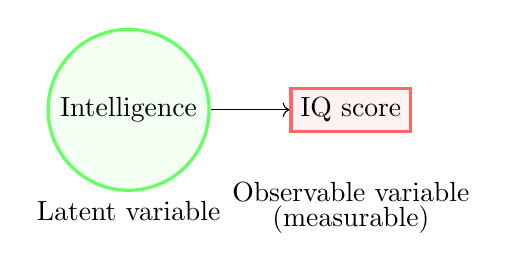
\begin{tikzpicture}[
  roundnode/.style={circle, draw=green!60, fill=green!5, very thick, minimum size=7mm},
  squarednode/.style={rectangle, draw=red!60, fill=red!5, very thick, minimum size=5mm},
]

% Nodes
\node[squarednode] (maintopic) {IQ score};
\node[roundnode] (intelligence) [left=of maintopic] {Intelligence};

% Text labels with positioning
\node [below=of intelligence, yshift=10mm] {Latent variable};
\node [below=of maintopic, yshift=5mm] {Observable variable};
\node [below=of maintopic, yshift=2mm] {(measurable)};

% Lines
\draw[->] (intelligence.east) -- (maintopic.west);

\end{tikzpicture}
\end{center}

This is why we must first measure or observe values $x$ (IQ score), so we can estimate $P(z|x)$ (intelligence). We know that the IQ score tests is Gaussian (normal) distributed with mean ($\mu$) of 100 with standard deviation ($\sigma$) of 15 points. We can say that $P(intelligence)$ is the prior distribution, because it represents our initial belief of possible values of intelligence. If we have little to no prior knowledge about intelligence, we can also assume it is uniform distributed, similarly to IQ score.

The posterior distribution $P(intelligence|IQ)$ is the updated belief about the possible values of intelligence \textbf{after} we observed their IQ score. It takes into account the prior knowledge and the information from observed variables, such as IQ.


\subsection{Likelihood function}
\label{appendix:likelihood_function}

When we talk about the likelihood function we usually mean that in the realm of generative models, our goal is to capture the underlying data distribution, hence we want to generate data ponits with similar likelihood to the training data distribution. 

The formal notion of likelihood function is: $L(x | \theta)$, which reflects the probability of a specific data point ($x$) being generated by the model with its current parameters ($\theta$). However, because we want to maximize this function, we can rewrite the goal as: $\underset{\theta}{\arg\max}\ L(x | \theta)$ (we want to find $\theta$ such that this function is maximum). Furthermore, in many cases, it's computationally more convenient to maximize the \textbf{log-likelihood} function, instead of the likelihood function itself, as the logarithm is a monotonic function (always increasing or decreasing, and therefor the log of the function is also monotonic):

\begin{equation}
\label{eq:mle}
    \hat{\theta}_{MLE} = \underset{\theta}{\arg\max} \ \log L(\mathbf{x} | \theta)
\end{equation}


In this regard, we might not want to directly estimate the likelihood function itself, but techniques like \textbf{maximum likelihood estimation (MLE)} (equation \ref{eq:mle}) can be used to optimize the model's parameters $\theta$ (can be used as a loss function). Calculating MLE directly is not feasible, however, because of intractability (high-integral).

Because of this, we usually use \textbf{Evidence Lower Bound (ELBO)} \ref{sec:elbo} estimation as alternative loss function. Other methods, such as adversarial training is also prominently used in GAN based model training.
\subsection{Variational Inference (VI)}
\label{appendix:variational_inference}

Variational inference (VI) is a technique used to approximate complex posterior distributions in Bayesian inference. Instead of directly maximizing the log-likelihood function, VI aims to minimize the \textbf{Kullback-Leibler (KL) divergence} between an approximate posterior distribution and the true posterior distribution (for instance, learn the distribution of 2D points that are generated by the model, which is estimation of another distribution we want the model to learn, for instance, Gaussian). This is often achieved by minimizing a proxy loss function, such as the \textbf{Evidence Lower Bound (ELBO)} (appendix \ref{appendix:elbo}), which is tractable (can be effectively computed) to optimize. By minimizing the ELBO, VI effectively guides the approximate posterior distribution towards the true posterior distribution.
\subsection{Kullback-Leibler (KL) divergence}
\label{appendix:kl_divergence}

\begin{figure}
    \centering
    \caption{Showcase of KL-Divergence of three different normal distributions. The divergence between two normal distributions can occur in both mean and variance. Mean (or expectation) is the center of the distribution, while variance is the spread of the distribution.}
    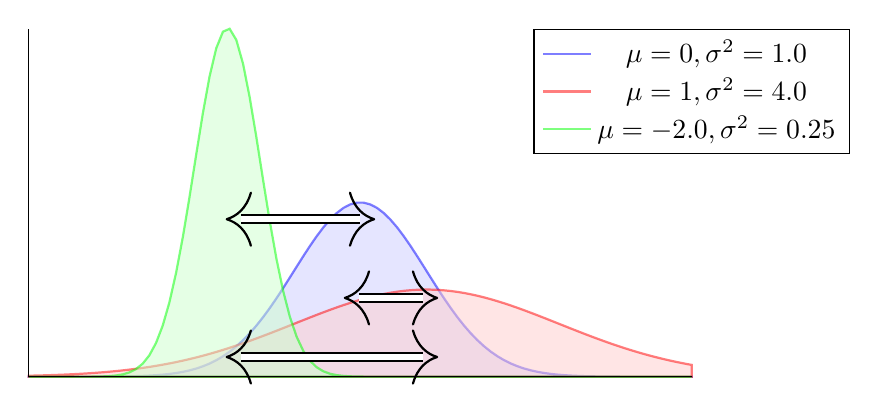
\begin{tikzpicture}
        \begin{axis} [
          no markers, 
          domain=-5:5, 
          samples=100,
          axis lines*=left, 
          height=6cm, 
          width=10cm,
          xtick=\empty, 
          ytick=\empty,
          enlargelimits=false, 
          clip=false, 
          axis on top,
          grid = major,
          legend style={at={(1,1)}, anchor=north, legend columns=1},
        ]

        % Define variables (mean, variance)
        \pgfmathsetmacro{\muA}{0}
        \pgfmathsetmacro{\sigmaA}{1}
        \pgfmathsetmacro{\varA}{\sigmaA^2}
        
        \pgfmathsetmacro{\muB}{1}
        \pgfmathsetmacro{\sigmaB}{2}
        \pgfmathsetmacro{\varB}{\sigmaB^2}
        
        \pgfmathsetmacro{\muC}{-2}
        \pgfmathsetmacro{\sigmaC}{0.5}
        \pgfmathsetmacro{\varC}{\sigmaC^2}
    
        % Blue
        \addplot[blue, thick, fill=blue!20, opacity=0.5] 
        {1/sqrt(2*pi*\sigmaA^2) * exp(-0.5 * ((x-\muA)/\sigmaA)^2)} \closedcycle;
        \addlegendentry{$\mu = \muA, \sigma^2 = \varA$};

        % Red
        \addplot[red, thick, fill=red!20, opacity=0.5] 
        {1/sqrt(2*pi*\sigmaB^2) * exp(-0.5 * ((x-\muB)/\sigmaB)^2)} \closedcycle;
        \addlegendentry{$\mu = \muB, \sigma^2 = \varB$};

        % Green
        \addplot[green, thick, fill=green!20, opacity=0.5] 
        {1/sqrt(2*pi*\sigmaC^2) * exp(-0.5 * ((x-\muC)/\sigmaC)^2)} \closedcycle;
        \addlegendentry{$\mu = \muC, \sigma^2 = \varC$};
        
        \end{axis}

        % Arrows between distributions
        % Blue, Green
        \draw[{<._[sep=-4pt]}-{_[sep=-4pt].>}, line width=0.8pt, double, double distance=2pt] (2.5,2) -- (4.4,2);
        % Green, Red
        \draw[{<._[sep=-4pt]}-{_[sep=-4pt].>}, line width=0.8pt, double, double distance=2pt] (2.5,0.25) -- (5.2,0.25);
        % Blue, Red
        \draw[{<._[sep=-4pt]}-{_[sep=-4pt].>}, line width=0.8pt, double, double distance=2pt] (4,1) -- (5.2,1);

    \end{tikzpicture}
\end{figure}

Kullback-Leibler (KL) divergence allows us to measure the difference between two probability distributions, $P$ and $Q$. It essentially quantifies how much information is lost when using distribution $Q$ to approximate distribution $P$.

In various applications, we deal with situations where we have a true underlying distribution (P) representing the actual data generation process, but we might not know its exact form. We might have another distribution (Q), perhaps a model we've built, that we want to use to represent or approximate the true distribution. KL divergence helps us understand how well Q captures the information present in P. In other words, \textbf{how much diverged the distribution Q is from the distribution P}. See figure \ref{fig:kl_divergence} for a visual representation.

The mathematical formula for KL-divergence is:

\begin{equation}
\label{eq:kl-divergence}
    D_{KL}(P || Q) = \sum_{x \in X} P(x) \cdot log(\frac{P(x)}{Q(x)})
\end{equation}

where $x \in X$ represents all the possible values within the data space ($X$).

A KL-divergence value of 0 indicate that the distribution $Q$ perfectly captures the distribution $P$, and larger numbers indicate higher disparity.

KL-divergence measures information lost, so if both $P,Q$ are Gaussian distributions with the same mean and standard deviation, we have no information lost. But if the standard deviation or the mean is different, KL-divergence measures that. On the other hand, directly integrating the distributions and measuring the area under the curve (AUC) will not show information loss if the standard deviation is the same, but the mean is different.


Other notations are used as well: $p_\theta(x_i), q_\phi(x_i)$. Most of the time we are dealing with small numbers in the probabilities, which will get multiplied with other small numbers, which may result in rounding to zero. So instead we generally compute \textbf{log-likelihood}: $log\ p_\theta(x_i), log\ q_\phi(x_i)$. Now to compare two distributions we can compute the difference: $log\ p_\theta(x_i) - log\ q_\phi(x_i)$ and if that subtraction result in zero that means that our approximated distribution $q$ is identical to ground truth $p$. We can rewrite it like so: 

\begin{equation}
\label{eq:log-likelihood}
    log\ [\frac{p_\theta(x_i)}{q_\phi(x_i)}]
\end{equation}

which is also sometimes called \textbf{log-likelihood ratio}.

In reality we are only interested in the \textbf{average difference} between $p_\theta$ and $q_\phi$. Because we are dealing with random variables $x \in X$, instead of average we say \textbf{expected value} of a random variable. Weighted average of instances of random variables is:

\begin{equation*}
    \mathbb{E}_{p_\theta} [X] = \sum_{i=1}^{\infty} x_i p_\theta(x_i)
\end{equation*}

where $x_i$ is the state of the random variable, and $p_\theta(x_i)$ is the weight (weight of contribution to the average). A more general formulation is given by:

\begin{equation*}
    \mathbb{E}_{p_\theta} [h(X)] = \sum_{i=1}^{\infty} h(x_i) p_\theta(x_i)
\end{equation*}

where $h(X), h(x_i)$ is a function of random variable $x_i \in X$. This formulation works for discrete random variable, here is the formulation for continuous random variable:

\begin{equation*}
    \mathbb{E}_{p_\theta} [h(X)] = \int_{\mathbb{R}} h(x) p_\theta(x) dx
\end{equation*}

Lets get back to the average likelihood (equation \ref{eq:log-likelihood}), we can set $h(X) = log\ [\frac{p_\theta(x_i)}{q_\phi(x_i)}]$ and we get:

\begin{equation*}
    \sum_{i=1}^{\infty} p_\theta(x_i) log\ [\frac{p_\theta(x_i)}{q_\phi(x_i)}]
\end{equation*}

where $p_\theta(x_i)$ is the weight. This equation is called the \textbf{KL-divergence}:

\begin{equation}
\label{eq:kl_divergence}
    \mathbb{E}_p [log\ \frac{p_\theta(x_i)}{q_\phi(x_i)}]
    =
    \sum_{i=1}^{\infty} p_\theta(x_i) log\ [\frac{p_\theta(x_i)}{q_\phi(x_i)}]
    =
    D_{KL} (p_\theta || q_\phi)
\end{equation}

In short, this is the expected value of the log-likelihood ratio (of discrete random variable). For continuous random variable we get similar formula:

\begin{equation}
\label{eq:kl_divergence_continous}
    \mathbb{E}_p [log\ \frac{p_\theta(x_i)}{q_\phi(x_i)}]
    =
    \int_{\mathbb{R}} p_\theta(x) log\ [\frac{p_\theta(x)}{q_\phi(x)}] dx
    =
    D_{KL} (p_\theta || q_\phi)
\end{equation}

One problem we are dealing with is the infinity space in both equations.  To get around it we can use the \textbf{law of large numbers} which says:

\begin{equation*}
    \frac{1}{N} \sum_{i=1}^N h(x_i) \approx \mathbb{E}_p [h(X)]
\end{equation*}

and we get:

\begin{equation}
    D_{KL} (p_\theta || q_\phi) \approx
    \frac{1}{N} \sum_{i=1}^N log\ [\frac{p_\theta(x_i)}{q_\phi(x_i)}]
\end{equation}

Credit to \cite{dk-divergence-math-explanation} for the math explanation.
\subsection{Evidence Lower Bound (ELBO)}
\label{appendix:elbo}

Evidence Lower Bound (ELBO) provides an efficient way to optimize and train models that are based on variational inference (often called latent models), like VAEs or GANs. ELBO is an estimation for the log-likelihood function, and since the likelihood function is intractable in latent models (that use latent variables $z$) to calculate directly, ELBO is used instead as approximation (its tractable). ELBO achieves this by setting a lower bound on the likelihood of observing data $x$. By maximizing ELBO we essentially optimize the model by maximizing likelihood.

As we saw in equation \ref{eq:vae_posterior} the likelihood function we want to optimize is:

\begin{equation}
    p(x) = \int p(x | z) \cdot p(z) dz
\end{equation}

where $p(x)$ is the likelihood of observing data $x$, $p(x | z)$ is probability of reconstructing $x$ given latent variable $z$,  $p(z)$ is the prior distribution of latent variable $z$, and the integral is over all possible values of $z$ (if $z$ is discrete, the integral is replaced by a sum).

The reason this integral is intractable is because it is computationally expensive to calculate the likelihood of all possible values of $z$. To solve this, we can use ELBO (also defined at equation \ref{eq:vae_elbo}), which is defined as:

\begin{equation}
    \text{ELBO} = \mathbb{E}_z[\log p(x | z)] - KL(q(z) \Vert p(z))
    \label{eq:elbo}
\end{equation}

where $\mathbb{E}_z[\log p(x | z)]$ is the expected reconstruction loss, and $KL(q(z) \Vert p(z))$ is the Kullback-Leibler divergence (see appendix \ref{appendix:kl_divergence}) between the approximate posterior $q(z)$ and the prior distribution $p(z)$.

The reason this is tractable is because we use mean (expectation) instead of integrating, and both the reconstruction loss and KL divergence are well defined and tractable. 


\subsection{VQ-VAE}

In listing \ref{lst:vq_codebook} we can see that the researchers divided the code vectors by number of embeddings, which normalizes the vectors in order to stabilize the training (the codebook vectors will have unit variance).

\begin{lstlisting}[language=Python, label=lst:vq_codebook, caption=Code of the quantisizer module of VQ-VAE paper. Shows the initialization of the codebook vectors.]
    class VectorQuantizer(nn.Module):
    """
    Discretization bottleneck part of the VQ-VAE.

    Inputs:
    - n_e : number of embeddings
    - e_dim : dimension of embedding
    - beta : commitment cost used in loss term, beta * ||z_e(x)-sg[e]||^2
    """

    def __init__(self, n_e, e_dim, beta):
        super(VectorQuantizer, self).__init__()
        self.n_e = n_e
        self.e_dim = e_dim
        self.beta = beta

        self.embedding = nn.Embedding(self.n_e, self.e_dim)
        self.embedding.weight.data.uniform_(-1.0 / self.n_e, 1.0 / self.n_e)
\end{lstlisting}




\begin{lstlisting}[language=Python, label=lst:vqvae_distance, caption=Euclidean distance calculation in VQ-VAE paper between embedding and codebook vectors $\Vert z-e \Vert$.]

    def forward(self, z):
        """
        Inputs the output of the encoder network z and maps it to a discrete 
        one-hot vector that is the index of the closest embedding vector e_j

        z (continuous) -> z_q (discrete)

        z.shape = (batch, channel, height, width)

        quantization pipeline:

            1. get encoder input (B,C,H,W)
            2. flatten input to (B*H*W,C)

        """
        # reshape z -> (batch, height, width, channel) and flatten
        z = z.permute(0, 2, 3, 1).contiguous()
        z_flattened = z.view(-1, self.e_dim)
        # distances from z to embeddings e_j (z - e)^2 = z^2 + e^2 - 2 e * z

        d = torch.sum(z_flattened ** 2, dim=1, keepdim=True) + \
            torch.sum(self.embedding.weight**2, dim=1) - 2 * \
            torch.matmul(z_flattened, self.embedding.weight.t())
    
\end{lstlisting}


\begin{lstlisting}[language=Python, label=lst:vqvae_loss, caption=Loss function as defined in the VQ-VAE paper (eq. \ref{eq:vq_loss}). The detach keyword is the stop gradient operation.]
    # compute loss for embedding
    loss = torch.mean((z_q.detach()-z)**2) + self.beta * \
        torch.mean((z_q - z.detach()) ** 2)
\end{lstlisting}



\begin{lstlisting}[language=Python, label=lst:vqvae_stop_gradients, caption=Allow gradients to flow through the snapping operation.]
    # preserve gradients
    z_q = z + (z_q - z).detach()
\end{lstlisting}

\end{document}